% Options for packages loaded elsewhere
\PassOptionsToPackage{unicode}{hyperref}
\PassOptionsToPackage{hyphens}{url}
\PassOptionsToPackage{dvipsnames,svgnames,x11names}{xcolor}
%
\documentclass[
  12pt,
]{book}
\usepackage{amsmath,amssymb}
\usepackage{iftex}
\ifPDFTeX
  \usepackage[T1]{fontenc}
  \usepackage[utf8]{inputenc}
  \usepackage{textcomp} % provide euro and other symbols
\else % if luatex or xetex
  \usepackage{unicode-math} % this also loads fontspec
  \defaultfontfeatures{Scale=MatchLowercase}
  \defaultfontfeatures[\rmfamily]{Ligatures=TeX,Scale=1}
\fi
\usepackage{lmodern}
\ifPDFTeX\else
  % xetex/luatex font selection
\fi
% Use upquote if available, for straight quotes in verbatim environments
\IfFileExists{upquote.sty}{\usepackage{upquote}}{}
\IfFileExists{microtype.sty}{% use microtype if available
  \usepackage[]{microtype}
  \UseMicrotypeSet[protrusion]{basicmath} % disable protrusion for tt fonts
}{}
\makeatletter
\@ifundefined{KOMAClassName}{% if non-KOMA class
  \IfFileExists{parskip.sty}{%
    \usepackage{parskip}
  }{% else
    \setlength{\parindent}{0pt}
    \setlength{\parskip}{6pt plus 2pt minus 1pt}}
}{% if KOMA class
  \KOMAoptions{parskip=half}}
\makeatother
\usepackage{xcolor}
\usepackage{color}
\usepackage{fancyvrb}
\newcommand{\VerbBar}{|}
\newcommand{\VERB}{\Verb[commandchars=\\\{\}]}
\DefineVerbatimEnvironment{Highlighting}{Verbatim}{commandchars=\\\{\}}
% Add ',fontsize=\small' for more characters per line
\usepackage{framed}
\definecolor{shadecolor}{RGB}{248,248,248}
\newenvironment{Shaded}{\begin{snugshade}}{\end{snugshade}}
\newcommand{\AlertTok}[1]{\textcolor[rgb]{0.94,0.16,0.16}{#1}}
\newcommand{\AnnotationTok}[1]{\textcolor[rgb]{0.56,0.35,0.01}{\textbf{\textit{#1}}}}
\newcommand{\AttributeTok}[1]{\textcolor[rgb]{0.13,0.29,0.53}{#1}}
\newcommand{\BaseNTok}[1]{\textcolor[rgb]{0.00,0.00,0.81}{#1}}
\newcommand{\BuiltInTok}[1]{#1}
\newcommand{\CharTok}[1]{\textcolor[rgb]{0.31,0.60,0.02}{#1}}
\newcommand{\CommentTok}[1]{\textcolor[rgb]{0.56,0.35,0.01}{\textit{#1}}}
\newcommand{\CommentVarTok}[1]{\textcolor[rgb]{0.56,0.35,0.01}{\textbf{\textit{#1}}}}
\newcommand{\ConstantTok}[1]{\textcolor[rgb]{0.56,0.35,0.01}{#1}}
\newcommand{\ControlFlowTok}[1]{\textcolor[rgb]{0.13,0.29,0.53}{\textbf{#1}}}
\newcommand{\DataTypeTok}[1]{\textcolor[rgb]{0.13,0.29,0.53}{#1}}
\newcommand{\DecValTok}[1]{\textcolor[rgb]{0.00,0.00,0.81}{#1}}
\newcommand{\DocumentationTok}[1]{\textcolor[rgb]{0.56,0.35,0.01}{\textbf{\textit{#1}}}}
\newcommand{\ErrorTok}[1]{\textcolor[rgb]{0.64,0.00,0.00}{\textbf{#1}}}
\newcommand{\ExtensionTok}[1]{#1}
\newcommand{\FloatTok}[1]{\textcolor[rgb]{0.00,0.00,0.81}{#1}}
\newcommand{\FunctionTok}[1]{\textcolor[rgb]{0.13,0.29,0.53}{\textbf{#1}}}
\newcommand{\ImportTok}[1]{#1}
\newcommand{\InformationTok}[1]{\textcolor[rgb]{0.56,0.35,0.01}{\textbf{\textit{#1}}}}
\newcommand{\KeywordTok}[1]{\textcolor[rgb]{0.13,0.29,0.53}{\textbf{#1}}}
\newcommand{\NormalTok}[1]{#1}
\newcommand{\OperatorTok}[1]{\textcolor[rgb]{0.81,0.36,0.00}{\textbf{#1}}}
\newcommand{\OtherTok}[1]{\textcolor[rgb]{0.56,0.35,0.01}{#1}}
\newcommand{\PreprocessorTok}[1]{\textcolor[rgb]{0.56,0.35,0.01}{\textit{#1}}}
\newcommand{\RegionMarkerTok}[1]{#1}
\newcommand{\SpecialCharTok}[1]{\textcolor[rgb]{0.81,0.36,0.00}{\textbf{#1}}}
\newcommand{\SpecialStringTok}[1]{\textcolor[rgb]{0.31,0.60,0.02}{#1}}
\newcommand{\StringTok}[1]{\textcolor[rgb]{0.31,0.60,0.02}{#1}}
\newcommand{\VariableTok}[1]{\textcolor[rgb]{0.00,0.00,0.00}{#1}}
\newcommand{\VerbatimStringTok}[1]{\textcolor[rgb]{0.31,0.60,0.02}{#1}}
\newcommand{\WarningTok}[1]{\textcolor[rgb]{0.56,0.35,0.01}{\textbf{\textit{#1}}}}
\usepackage{longtable,booktabs,array}
\usepackage{calc} % for calculating minipage widths
% Correct order of tables after \paragraph or \subparagraph
\usepackage{etoolbox}
\makeatletter
\patchcmd\longtable{\par}{\if@noskipsec\mbox{}\fi\par}{}{}
\makeatother
% Allow footnotes in longtable head/foot
\IfFileExists{footnotehyper.sty}{\usepackage{footnotehyper}}{\usepackage{footnote}}
\makesavenoteenv{longtable}
\usepackage{graphicx}
\makeatletter
\def\maxwidth{\ifdim\Gin@nat@width>\linewidth\linewidth\else\Gin@nat@width\fi}
\def\maxheight{\ifdim\Gin@nat@height>\textheight\textheight\else\Gin@nat@height\fi}
\makeatother
% Scale images if necessary, so that they will not overflow the page
% margins by default, and it is still possible to overwrite the defaults
% using explicit options in \includegraphics[width, height, ...]{}
\setkeys{Gin}{width=\maxwidth,height=\maxheight,keepaspectratio}
% Set default figure placement to htbp
\makeatletter
\def\fps@figure{htbp}
\makeatother
\setlength{\emergencystretch}{3em} % prevent overfull lines
\providecommand{\tightlist}{%
  \setlength{\itemsep}{0pt}\setlength{\parskip}{0pt}}
\setcounter{secnumdepth}{5}
\usepackage{booktabs}
\usepackage{tcolorbox}
\usepackage{ifthen}
\usepackage{graphicx}
\usepackage{framed,color}
\usepackage{fvextra}
\usepackage{titlesec}
\usepackage{longtable} 

\usepackage{Alegreya} 
\usepackage[scale=.7]{sourcecodepro}

\usepackage[left=3cm,right=3cm,top=3cm,bottom=3cm]{geometry}

\renewenvironment{figure}
  {\begin{figure}\centering}
  {\end{figure}}

\definecolor{definition_frame}{RGB}{50, 84, 129}
\definecolor{definition_color}{RGB}{218, 228, 242}
\definecolor{important_frame}{RGB}{196, 184, 16}
\definecolor{important_color}{RGB}{247, 247, 208}
\definecolor{note_frame}{RGB}{27, 5, 5}
\definecolor{note_color}{RGB}{224, 224, 224}
\definecolor{warning_frame}{RGB}{232, 27, 27}
\definecolor{warning_color}{RGB}{253, 174, 174}

\newenvironment{infobox}[1] 
  {
  \begin{itemize}
  \renewcommand{\labelitemi}{
    \raisebox{-.4\height}[0pt][0pt]{
      {\setkeys{Gin}{width=2.5em,keepaspectratio}
      \includegraphics{images/#1}}
    }
  }
  \setlength{\fboxsep}{1em}

  \ifthenelse{\equal{#1}{magnifying_glass}}{
    \begin{tcolorbox}[colback=definition_color, colframe=definition_frame, coltext=black, top=10pt, bottom=10pt, left=35pt, right=10pt, arc=4pt, before skip=10pt, after skip=10pt]
    \setlength{\parskip}{1.5ex}
    \setlength{\parindent}{0pt} 
  }{
    \ifthenelse{\equal{#1}{important_exclamation}}{
      \begin{tcolorbox}[colback=important_color, colframe=important_frame, coltext=black, top=10pt, bottom=10pt, left=45pt, right=10pt, arc=4pt, before skip=10pt, after skip=10pt]
      \setlength{\parskip}{1.5ex}
      \setlength{\parindent}{0pt} 
    }{
      \ifthenelse{\equal{#1}{bell_note}}{
        \begin{tcolorbox}[colback=note_color, colframe=note_frame, coltext=black, top=10pt, bottom=10pt, left=40pt, right=10pt, arc=4pt, before skip=10pt, after skip=10pt]
        \setlength{\parskip}{1.5ex}
        \setlength{\parindent}{0pt} 
      }{
        \begin{tcolorbox}[colback=warning_color, colframe=warning_frame, coltext=black, top=10pt, bottom=10pt, left=45pt, right=10pt, arc=4pt, before skip=10pt, after skip=10pt]
        \setlength{\parskip}{1.5ex}
        \setlength{\parindent}{0pt} 
      }
    }
  }
  \item
  }
  {
  \end{tcolorbox}
  \end{itemize}
}

\DefineVerbatimEnvironment{Highlighting}{Verbatim}{
    commandchars=\\\{\},
    breaklines, breaknonspaceingroup, breakanywhere}
    
\let\cleardoublepage\clearpage

\titleformat{\chapter}[hang]
  {\normalfont\huge\bfseries}{\thechapter}{2em}{}
\titlespacing*{\chapter}{0pt}{\baselineskip}{0.5\baselineskip}
\usepackage{booktabs}
\usepackage{longtable}
\usepackage{array}
\usepackage{multirow}
\usepackage{wrapfig}
\usepackage{float}
\usepackage{colortbl}
\usepackage{pdflscape}
\usepackage{tabu}
\usepackage{threeparttable}
\usepackage{threeparttablex}
\usepackage[normalem]{ulem}
\usepackage{makecell}
\usepackage{xcolor}
\ifLuaTeX
  \usepackage{selnolig}  % disable illegal ligatures
\fi
\usepackage[]{natbib}
\bibliographystyle{plainnat}
\usepackage{bookmark}
\IfFileExists{xurl.sty}{\usepackage{xurl}}{} % add URL line breaks if available
\urlstyle{same}
\hypersetup{
  pdftitle={UCSB ECON 145 Autograder Manual},
  pdfauthor={Riley Berman, Alex Zhao, \& 2024 ECON 145 Summer Team},
  colorlinks=true,
  linkcolor={Maroon},
  filecolor={Maroon},
  citecolor={Blue},
  urlcolor={Blue},
  pdfcreator={LaTeX via pandoc}}

\title{UCSB ECON 145 Autograder Manual}
\author{Riley Berman, Alex Zhao, \& 2024 ECON 145 Summer Team}
\date{Last Updated: 2025-04-03}

\begin{document}
\maketitle

{
\hypersetup{linkcolor=}
\setcounter{tocdepth}{1}
\tableofcontents
}
\chapter*{Preface}\label{preface}
\addcontentsline{toc}{chapter}{Preface}

This manual outlines how to develop an autograder for ECON 145, ``Data Wrangling for Economics,'' at the \href{https://econ.ucsb.edu/programs/undergraduate/courses}{University of California, Santa Barbara}. Many of the techniques presented here can be applied to \emph{any R-based autograder}.

You can read the manual online or download the \textbf{pdf} using the toolbar's ``download'' icon. For the best reading experience, the online version is recommended. In the online version, code blocks are scrollable and include a copy button in the top-right corner. Code blocks may look a little wonky in the pdf version.

This manual may contain mistakes or sections that require updates or improvement. Use the toolbar's ``edit'' icon to open the GitHub repository and submit issues or pull requests.

\section*{Acknowledgements}\label{Acknowledgements}
\addcontentsline{toc}{section}{Acknowledgements}

This guidebook aims to reflect new conventions and up-to-date techniques used in ECON 145 autograders developed by the 2024 ECON 145 Summer Team of \textbf{Jack Keefer (Head TA), Alex Zhao, Riley Berman, Shreya Sinha, and Michal Snopek}. We are extremely grateful for the foundational work established by previous ECON 145 TAs.

Special thanks to Alex Zhao and his excellent \texttt{autograder\_manual\_2024.pdf}, which laid the groundwork for this manual.

The author would also like to thank Xiao Yang for her invaluable feedback and suggestions.

\begin{flushright}
Riley Berman
\end{flushright}

\chapter{Introduction}\label{introduction}

This manual explains how to build an autograder for \href{https://econ.ucsb.edu/programs/undergraduate/courses}{UCSB ECON 145} coding assignments.

\begin{infobox}{magnifying_glass}
\textbf{WHAT IS AN AUTOGRADER?}

In this manual, an \emph{autograder}, or \emph{autograder program}, is an R script that grades a student's R-based assignment and provides question-specific feedback. It runs alongside a set of supporting R scripts, collectively known as the \emph{autograder infrastructure.}

See \hyperref[Autograder-Conventions]{Autograder Conventions} for more details.

\end{infobox}

In ECON 145 assignments, coding questions are classified as either \hyperref[Public-Questions]{\textbf{Public}} or \hyperref[Private-Questions]{\textbf{Private}}.

\begin{itemize}
\item
  For any Public Question, we write custom ``Checks'' -- lines of code that test for specific answer attributes -- that evaluate the student's answer and return \emph{constructive and dynamic feedback}.
\item
  For any Private Question, we use a set of premade functions that evaluate the student's answer and return \emph{necessary and basic feedback}.
\end{itemize}

Accordingly, most of this manual focuses on writing Checks for Public Questions.

We will look at grading four types of data structures: tibbles, vectors, lists, and plots. Moreover, as the majority of ECON 145 assignment questions are tibble-based, we direct our attention to grading tibbles.

For fellow ECON 145 TAs, we recommend skimming through \hyperref[resources]{\texttt{00-manual1.pdf}} and \hyperref[resources]{\texttt{how\_to\_create\_an\_autograder\_2024.pdf}} for an overview of the autograder infrastructure.

\begin{infobox}{bell_note}
\textbf{Note}:

Unless noted, all references and examples come from the Fall 2024 ECON 145 course.

\end{infobox}

\chapter{Autograder Conventions}\label{Autograder-Conventions}

The \emph{autograder infrastructure}, or \emph{autograder system}, is a set of R scripts that work together to implement the \emph{autograder} -- that is, to evaluate a student's R-assignment and return question-specific feedback through the Gradescope platform.

Sometimes, the term ``autograder'' is used to refer to the entire system, but I will try to stick to this division throughout the manual.

\begin{infobox}{important_exclamation}
\textbf{WHY FOCUS ON JUST THE AUTOGRADER?}

TAs primarily work on writing the autograder, while the Head TA handles the integration of the autograder and its infastructure with Gradescope.

\end{infobox}

A quick overview of the \hyperref[DGP.R]{DGP.R} file will also be provided, which \emph{every TA} should review.

For implementation and testing details of the autograder, refer to the document\hyperref[resources]{\texttt{how\_to\_create\_an\_autograder\_2024.pdf}}.

\section{General Structure}\label{general-structure}

Generally, an autograder script will look something like:

\begin{Shaded}
\begin{Highlighting}[]
\FunctionTok{rm}\NormalTok{(}\AttributeTok{list =} \FunctionTok{ls}\NormalTok{())}

\CommentTok{\#{-}{-}{-}{-}{-}{-}{-}{-}{-}{-}{-}{-}{-}{-}Set This{-}{-}{-}{-}{-}{-}\#}
\CommentTok{\#loc       \textless{}{-} "local" \# either "local", or "gradescope"}
\NormalTok{loc       }\OtherTok{\textless{}{-}} \StringTok{"gradescope"}

\CommentTok{\#{-}{-}{-}{-}{-}{-}DON\textquotesingle{}T TOUCH THIS{-}{-}{-}{-}{-}{-}\#}

\CommentTok{\#Setting working directory to source file location}
\ControlFlowTok{if}\NormalTok{(loc}\SpecialCharTok{==}\StringTok{"local"}\NormalTok{)\{}
  \FunctionTok{setwd}\NormalTok{(}\FunctionTok{dirname}\NormalTok{(rstudioapi}\SpecialCharTok{::}\FunctionTok{getSourceEditorContext}\NormalTok{()}\SpecialCharTok{$}\NormalTok{path))}
\NormalTok{\}}
\FunctionTok{source}\NormalTok{(}\StringTok{"inputs.R"}\NormalTok{)}
\FunctionTok{source}\NormalTok{(}\FunctionTok{paste0}\NormalTok{(here}\SpecialCharTok{::}\FunctionTok{here}\NormalTok{(),}\StringTok{"/helper\_functions/autograder\_setup.R"}\NormalTok{,}\StringTok{""}\NormalTok{))}
\FunctionTok{source}\NormalTok{(}\FunctionTok{paste0}\NormalTok{(here}\SpecialCharTok{::}\FunctionTok{here}\NormalTok{(),}\StringTok{"/helper\_functions/misc\_helper\_functions.R"}\NormalTok{,}\StringTok{""}\NormalTok{))}
\FunctionTok{source}\NormalTok{(}\StringTok{"inputs.R"}\NormalTok{)}

\CommentTok{\#{-}{-}{-}{-}{-}{-}{-}{-}{-}{-}{-}{-}{-}{-}{-}{-}{-}{-}{-}{-}{-}{-}{-}{-}{-}{-}{-}{-}\#}

\ControlFlowTok{if}\NormalTok{(status}\SpecialCharTok{!=}\StringTok{"Error"}\NormalTok{)\{}
  
  \CommentTok{\#Answer Key Goes Here...  }
  
  \CommentTok{\#Question 1 Solution}
  
  \CommentTok{\#Question 2 Solution, etc. }
  
  \CommentTok{\#Autograder Code Goes Here... }
  
  \CommentTok{\#Testing Student\textquotesingle{}s Question 1 Against Question 1 Solution}
  
  \CommentTok{\#Testing Student\textquotesingle{}s Question 2 Against Question 2 Solution, etc.  }
  
  \CommentTok{\# {-}{-}{-}{-}{-}{-}{-}{-}{-}{-}{-}{-}{-}{-}{-}{-}{-}{-}{-}{-}{-}{-}{-}{-}{-}{-}{-}{-}{-}{-}{-}{-}{-}{-}{-}{-}{-}{-}{-}{-}{-}{-}{-}{-}{-}{-}{-}{-}{-}{-}{-}{-}{-}{-}{-}{-}{-}{-}{-} \#}
  
  \FunctionTok{JSONmaker}\NormalTok{(test.results, loc)}
\NormalTok{\}}
\end{Highlighting}
\end{Shaded}

Under \texttt{\#Answer\ Key\ Goes\ Here...}, TAs insert the assignment solutions. To distinguish solutions from the student's answers (so they can be compared), we tend to follow the convention of appending ``\texttt{\_test}'' to the answer key's variable name.

\begin{itemize}
\tightlist
\item
  For example, if Question 1 on the homework asks the student to create a tibble named \texttt{basketball\_data}, the answer key's corresponding tibble will be named \texttt{basketball\_data\_test}.
\end{itemize}

Under \texttt{\#Autograder\ Code\ Goes\ Here...}, TAs insert their code for the autograder. Question by question, this code will compare the student's solution to the corresponding answer key. As a reminder\ldots{}

\begin{itemize}
\item
  For any Public Question, we program a series of ``Checks'' (lines of code) to test the student's answer for a \emph{range of attributes} and return dynamic feedback. See \hyperref[Public-Questions]{Public Questions}.
\item
  For any Private Question, we employ a group of built-in functions to test the student's answer for a \emph{fixed set of attributes} and return basic feedback. See \hyperref[Private-Questions]{Private Questions}.
\end{itemize}

\begin{infobox}{warning}
The autograder \textbf{only} evaluates the student's final result, the R object -- it does not grade the code required to produce it.

Accordingly, students can receive full credit for a question even if their code is vastly different from the answer key. The feedback our Checks generate guide students towards the \emph{recommended, class-based} solution.

The student's R object \textbf{does not} need to be identical to the answer key to receive full credit. See \hyperref[Correct-Check]{Correct Check} for more details.

\end{infobox}

\section{What is test.results?}\label{test.results}

The autograder infrastructure has provided a \texttt{test.results} data frame to store and display feedback from our Checks.

When writing autograder code for \emph{any} question, we \emph{always} first initialize the question's default \texttt{test.results}.

For example, to initialize Question 1's \texttt{test.results}, we write the following line:

\begin{Shaded}
\begin{Highlighting}[]
\CommentTok{\#Testing Student\textquotesingle{}s Question 1 Against Question 1 Solution}
\NormalTok{test.results[}\DecValTok{1}\NormalTok{, ] }\OtherTok{\textless{}{-}} \FunctionTok{c}\NormalTok{(}\StringTok{"Part 1 Question 1 (Public)"}\NormalTok{, }\DecValTok{0}\NormalTok{, }\DecValTok{20}\NormalTok{, }\StringTok{"Try again."}\NormalTok{)}
\end{Highlighting}
\end{Shaded}

where each element of \texttt{test.results{[}\#,\ {]}} is as follows:

\renewcommand{\arraystretch}{2}

\begin{longtable}{ll}
\toprule
\textbf{Element} & \textbf{Description}\\
\midrule
\cellcolor{gray!10}{1} & \cellcolor{gray!10}{the question's number}\\
\hline
"Part 1 Question 1 (Public)" & the question's displayed part, number and type (Private/Public)\\
\hline
\cellcolor{gray!10}{0} & \cellcolor{gray!10}{the question's default score}\\
\hline
20 & the question's maximum score\\
\hline
\cellcolor{gray!10}{"Try again."} & \cellcolor{gray!10}{the default feedback message}\\
\bottomrule
\end{longtable}

It is important to note that a question's \emph{displayed number} may differ from its \emph{question number}, especially in the case of multi-part questions.

\textbf{Recommendation}: If students would greatly benefit from a very specific hint (e.g., using a certain function), you can include it in the default feedback message to ensure they see it in the case that none of the Checks trigger.

After initializing a question's \texttt{test.results{[}\#,\ {]}}, we can update it through indexing.

\begin{itemize}
\tightlist
\item
  For example, if the student's Question 1 is correct, we can update \texttt{test.results{[}1,\ {]}} to award them full score with the following line:
\end{itemize}

\begin{Shaded}
\begin{Highlighting}[]
\CommentTok{\#Modifying the score for Question 1}
\NormalTok{test.results[}\DecValTok{1}\NormalTok{, }\DecValTok{2}\NormalTok{] }\OtherTok{\textless{}{-}} \DecValTok{20}
\end{Highlighting}
\end{Shaded}

Similarly, we can modify the feedback message through the following line:

\begin{Shaded}
\begin{Highlighting}[]
\CommentTok{\#Modifying the feedback message for Question 1}
\NormalTok{test.results[}\DecValTok{1}\NormalTok{, }\DecValTok{4}\NormalTok{] }\OtherTok{\textless{}{-}} \StringTok{"Insert feedback message here!"}
\end{Highlighting}
\end{Shaded}

\begin{infobox}{bell_note}
\textbf{Note}:

For most of the sample code provided for \hyperref[Public-Questions]{Public Questions}, we will be updating \texttt{test.results{[}2,\ {]}} (i.e., Question 2).

\end{infobox}

\chapter{Public Questions}\label{Public-Questions}

Public Question Checks are designed to give students \emph{constructive and dynamic feedback} that help them to improve their answer and progress toward the solution.

To achieve this, Public Questions will require multiple Checks that test for particular answer properties and generate tailored feedback.

There are two categories of Checks: \hyperref[General-Checks]{\textbf{General}} and \hyperref[Special-Checks]{\textbf{Special Checks}}.

\phantomsection\label{General-Checks}
\begin{infobox}{magnifying_glass}
\textbf{WHAT IS A GENERAL CHECK?}

A \emph{General Check} tests for a \emph{common} answer property that applies across many, if not all, questions.

For example, all questions require the student to label their variable \emph{a specific name}. Accordingly, for any Public (or Private) Question, a General Check should alert the student if their variable name does not match the name specified in the instructions (this is the \hyperref[Name-Check]{Name Check}).

\textbf{We implement General Checks for all Public Questions.}

\end{infobox}

\phantomsection\label{Special-Checks}
\begin{infobox}{magnifying_glass}
\textbf{WHAT IS A SPECIAL CHECK?}

A \emph{Special Check} tests for an answer property \emph{unique} to the given question.

For example, if a Public Question asks the student to multiply a column by a certain number, a Special Check should alert them if they use a specific, improper scale (this is the \hyperref[Calculation-Check]{Calculation Check}). Note that this Check is \emph{specific to this question} and is not a general answer property.

\textbf{We implement Special Checks on a question-by-question basis.}

\end{infobox}

\begin{infobox}{bell_note}
\textbf{Note}:

General Checks are denoted with a ``(G)'' and Special Checks with an ``(S)''.

\end{infobox}

\section{General Form}\label{general-form}

A Public Question's autograder code \emph{combines} General and Special Checks like the following:

\begin{Shaded}
\begin{Highlighting}[]
\CommentTok{\#Public Question 2 Autograder Code}
\CommentTok{\#Testing Student\textquotesingle{}s Question 2 Against Question 2 Solution}

\CommentTok{\#Initializing test.results[2, ]}
\NormalTok{test.results[}\DecValTok{2}\NormalTok{, ] }\OtherTok{\textless{}{-}} \FunctionTok{c}\NormalTok{(}\StringTok{"Part 1 Question 2 (Public)"}\NormalTok{, }\DecValTok{0}\NormalTok{, }\DecValTok{20}\NormalTok{, }\StringTok{"Try again."}\NormalTok{)}

\CommentTok{\#General Check 1}
\ControlFlowTok{if}\NormalTok{(test\_condition)\{ }
\NormalTok{  code... }
\CommentTok{\#General Check 2}
\NormalTok{\}}\ControlFlowTok{else} \ControlFlowTok{if}\NormalTok{(test\_condition)\{ }
\NormalTok{  code...}
\CommentTok{\#Special Check 1}
\NormalTok{\}}\ControlFlowTok{else} \ControlFlowTok{if}\NormalTok{(test\_condition)\{ }
\NormalTok{  code...}
\CommentTok{\#Special Check 2}
\NormalTok{\}}\ControlFlowTok{else} \ControlFlowTok{if}\NormalTok{(test\_condition)\{ }
\NormalTok{  code...}
\NormalTok{.}
\NormalTok{.}
\NormalTok{.}
\CommentTok{\#Last General Check }
\NormalTok{\}}\ControlFlowTok{else} \ControlFlowTok{if}\NormalTok{(test\_condition)\{}
\NormalTok{  code... }
\NormalTok{\}}
\end{Highlighting}
\end{Shaded}

We will learn a variety of Checks in the following sections.

\section{Name Check (G)}\label{Name-Check}

\textbf{Purpose}: Checks whether the student's variable has the correct name.

\textbf{Motivation}: All questions require the student to give their variable a specific name. Without a Name Check, the autograder can't match and compare the student's answer to the answer key -- and other Checks that rely on a correctly named student variable, such as the \hyperref[Column-Name-Check]{Column Name Check}, may error out as a result.

\begin{Shaded}
\begin{Highlighting}[]
\CommentTok{\#Name Check Example}

\ControlFlowTok{if}\NormalTok{(}\FunctionTok{is.error}\NormalTok{(variable\_name))\{ }
\NormalTok{  test.results[}\DecValTok{2}\NormalTok{, }\DecValTok{4}\NormalTok{] }\OtherTok{\textless{}{-}} \StringTok{"\textasciigrave{}variable\_name\textasciigrave{} is not found. Please make sure the variable is named correctly. (Any additional feedback as needed.)"}
\NormalTok{\}}
\end{Highlighting}
\end{Shaded}

\subsubsection*{Technicals}\label{technicals}
\addcontentsline{toc}{subsubsection}{Technicals}

\begin{infobox}{important_exclamation}
\textbf{Always include the Name Check.}

If there is no \hyperref[Prerequisite-Check]{Prerequisite Check}, place this Check first (the \texttt{if} statement); otherwise, it should follow immediately after (the first \texttt{else\ if} statement).

\end{infobox}

\begin{infobox}{bell_note}
\textbf{Note}:

The \texttt{is.error()} function comes from the \texttt{berryFunctions} package \citep{R-berryFunctions}. For the ECON 145 autograder, this library should already be loaded in from the file \texttt{helper\_functions/packages.R}.

\end{infobox}

\section{Prerequisite Check (G)}\label{Prerequisite-Check}

\textbf{Purpose}: Checks whether the student got the prerequisite question correct.

\textbf{Motivation}: Many questions build on previous ones. If the student did not get the ``prerequisite'' question(s) correct, their current answer is likely incorrect as well. This Check prompts the student to revisit their earlier work. Since the prerequisite question is often the previous question, this Check is also called the ``Previous Question Check.''

\begin{Shaded}
\begin{Highlighting}[]
\CommentTok{\#Prerequisite Check Example}

\ControlFlowTok{else} \ControlFlowTok{if}\NormalTok{(test.results[}\DecValTok{1}\NormalTok{, }\DecValTok{2}\NormalTok{] }\SpecialCharTok{==} \DecValTok{0}\NormalTok{)\{ }\CommentTok{\#If Question 1 is incorrect...}
\NormalTok{  test.results[}\DecValTok{2}\NormalTok{, }\DecValTok{4}\NormalTok{] }\OtherTok{\textless{}{-}} \StringTok{"This question depends on Question 1 being correct. Try again. (Any additional feedback as needed.)"}
\NormalTok{\}}
\end{Highlighting}
\end{Shaded}

\subsubsection*{Technicals}\label{technicals-1}
\addcontentsline{toc}{subsubsection}{Technicals}

\begin{infobox}{important_exclamation}
Place the Prerequisite Check first so it is triggered first.

Don't use the Prerequisite Check for the first question, or for any stand-alone questions.

\end{infobox}

\textbf{Recommendation}: If the assignment has multiple parts (e.g., Part 1, Part 2, etc.), you should clarify where the prerequisite question is in the feedback message of \texttt{test.results{[}\#,\ 4{]}}.

\section{Structure Check (G)}\label{Structure-Check}

\textbf{Purpose}: Checks whether the student's variable has the correct data structure (e.g., list, tibble). In most cases, this will be a tibble.

\textbf{Motivation}: Using the wrong data structure may cause the autograder to reject an otherwise correct-looking answer. It can also break Checks that expect a certain data structure, like the \hyperref[Calculation-Check]{Calculation Check}.

\begin{Shaded}
\begin{Highlighting}[]
\CommentTok{\#Structure Check Example }

\CommentTok{\#For a tibble...}
\ControlFlowTok{else} \ControlFlowTok{if}\NormalTok{(}\SpecialCharTok{!}\FunctionTok{is\_tibble}\NormalTok{(variable\_name))\{}
\NormalTok{  test.results[}\DecValTok{2}\NormalTok{, }\DecValTok{4}\NormalTok{] }\OtherTok{\textless{}{-}} \StringTok{"Make sure \textasciigrave{}variable\_name\textasciigrave{} is a tibble. (Any additional feedback as needed.)"}
\NormalTok{\}}

\CommentTok{\#For a list...}
\CommentTok{\#\textasciigrave{}janitor::tabyl()\textasciigrave{} and other \textasciigrave{}janitor\textasciigrave{} related functions produce a list, not a tibble}
\CommentTok{\#In this case, the Structure Check should check for a list, like below}
\ControlFlowTok{else} \ControlFlowTok{if}\NormalTok{(}\SpecialCharTok{!}\FunctionTok{is\_list}\NormalTok{(variable\_name))\{}
\NormalTok{  test.results[}\DecValTok{2}\NormalTok{, }\DecValTok{4}\NormalTok{] }\OtherTok{\textless{}{-}} \StringTok{"Make sure \textasciigrave{}variable\_name\textasciigrave{} is a list. (Any additional feedback as needed.)"}
\NormalTok{\}}
\end{Highlighting}
\end{Shaded}

\subsubsection*{Technicals}\label{technicals-2}
\addcontentsline{toc}{subsubsection}{Technicals}

\begin{infobox}{important_exclamation}
\textbf{Always include the Structure Check.}

A common mistake students make is using \texttt{read.csv()} instead of \texttt{read\_csv()} when loading datasets into R. The problem is that the former returns a \emph{data frame}, while the latter returns a \emph{tibble} (a special, modern type of data frame).

\end{infobox}

There are slight differences \citep{wickham2016} between how general data frames and tibbles behave in R. For example, tibbles do not change the type of the inputs (e.g., they never convert strings to factors) and they allow for non-syntactic names (e.g., names with spaces). These small differences may cause the autograder to reject the student's answer or inconvenience the student when solving the assignment.

For Public Questions that involve \texttt{janitor::tabyl()} and other \texttt{janitor} related functions (e.g., \texttt{adorn\_pct\_formatting}, \texttt{adorn\_totals}), the student's answer will be a \emph{list, not a tibble.} In this case, the Structure Check should check for a list. For three-way \texttt{tabyl} lists, see \hyperref[private_tabyl_grader]{\texttt{private\_tabyl\_grader()}}.

\textbf{Recommendation}: For questions that involve loading data into R, tack on a reminder in \texttt{test.results{[}\#,\ 4{]}} for the student to use \texttt{read\_csv()} instead of \texttt{read.csv()}.

\section{Column Name Check (G)}\label{Column-Name-Check}

\textbf{Purpose}: Dynamically checks whether the column names in the student's tibble (A) match those in the answer key (B). We break this test into two parts:

\begin{enumerate}
\def\labelenumi{\arabic{enumi}.}
\item
  Test whether \(B \not\subset A\), that is, if the student's tibble is missing any column names from the answer key.
\item
  Test whether \(A \not\subset B\), that is, if the student's tibble has any additional column names not in the answer key.
\end{enumerate}

\textbf{Motivation}: Many questions involve the deletion or addition of columns in a tibble. Students often misname, omit, or forget to remove such columns. This Check helps catch these issues early, reducing the time students spends sifting through their code for a simple mistake (e.g., a typo).

\begin{Shaded}
\begin{Highlighting}[]
\CommentTok{\#Column Name Check Example}

\CommentTok{\#First Test (B not in A)}
\ControlFlowTok{else} \ControlFlowTok{if}\NormalTok{(}\SpecialCharTok{!}\FunctionTok{all}\NormalTok{(}\FunctionTok{colnames}\NormalTok{(variable\_name\_test) }\SpecialCharTok{\%in\%} \FunctionTok{colnames}\NormalTok{(variable\_name)))\{}
\NormalTok{  test.results[}\DecValTok{2}\NormalTok{, }\DecValTok{4}\NormalTok{] }\OtherTok{\textless{}{-}} \FunctionTok{paste0}\NormalTok{(}\FunctionTok{c}\NormalTok{(}\StringTok{"The following column(s) should be in \textasciigrave{}variable\_name\textasciigrave{}, but they were not found in your answer: "}\NormalTok{,}
    \FunctionTok{paste0}\NormalTok{(}\FunctionTok{colnames}\NormalTok{(variable\_name\_test)[}\SpecialCharTok{!}\NormalTok{(}\FunctionTok{colnames}\NormalTok{(variable\_name\_test) }\SpecialCharTok{\%in\%} \FunctionTok{colnames}\NormalTok{(variable\_name))], }\AttributeTok{collapse =} \StringTok{", "}\NormalTok{), }\StringTok{". (Any additional feedback as needed.)"}\NormalTok{), }\AttributeTok{collapse =} \StringTok{""}\NormalTok{)}
\NormalTok{\} }

\CommentTok{\#Second Test (A not in B)}
\ControlFlowTok{else} \ControlFlowTok{if}\NormalTok{(}\SpecialCharTok{!}\FunctionTok{all}\NormalTok{(}\FunctionTok{colnames}\NormalTok{(variable\_name) }\SpecialCharTok{\%in\%} \FunctionTok{colnames}\NormalTok{(variable\_name\_test)))\{}
\NormalTok{  test.results[}\DecValTok{2}\NormalTok{, }\DecValTok{4}\NormalTok{] }\OtherTok{\textless{}{-}} \FunctionTok{paste0}\NormalTok{(}\FunctionTok{c}\NormalTok{(}\StringTok{"The following column(s) should not be in \textasciigrave{}variable\_name\textasciigrave{}, but they were found in your answer: "}\NormalTok{,}
    \FunctionTok{paste0}\NormalTok{(}\FunctionTok{colnames}\NormalTok{(variable\_name)[}\SpecialCharTok{!}\NormalTok{(}\FunctionTok{colnames}\NormalTok{(variable\_name) }\SpecialCharTok{\%in\%} \FunctionTok{colnames}\NormalTok{(variable\_name\_test))],}
    \AttributeTok{collapse =} \StringTok{", "}\NormalTok{), }\StringTok{". (Any additional feedback as needed.)"}\NormalTok{), }\AttributeTok{collapse =} \StringTok{""}\NormalTok{)}
\NormalTok{\}}
\end{Highlighting}
\end{Shaded}

\subsubsection*{Technicals}\label{technicals-3}
\addcontentsline{toc}{subsubsection}{Technicals}

\begin{infobox}{important_exclamation}
\textbf{Always include the Column Name Check.}

This Check is \emph{essential} for subsequent Checks that rely on the student's answer having correctly named columns, like the \hyperref[Correct-Check]{Correct Check}.

\end{infobox}

While the Column Name Check is designed for tibbles, it can easily be adapted for named lists by swapping \texttt{colnames()} for \texttt{names()}. Please note that lists should \emph{first} be checked if they are named through a \texttt{NULL} Check like \texttt{is.null(names(variable\_name))}.

\section{Row \& Column Check (G)}\label{Row-Column-Check}

\textbf{Purpose}: Checks whether the student's tibble has the same number of rows and columns as the answer key.

\textbf{Motivation}: Many questions involve the deletion or addition of rows and/or columns in a tibble. This Check alerts students, rather broadly, to a discrepancy in their number of rows and columns. Row and column mismatches can cause Checks, like the \hyperref[Correct-Check]{Correct Check}, to error out.

\begin{Shaded}
\begin{Highlighting}[]
\CommentTok{\#Row \& Column Check Example}

\CommentTok{\#Row Check}
\ControlFlowTok{else} \ControlFlowTok{if}\NormalTok{(}\FunctionTok{nrow}\NormalTok{(variable\_name) }\SpecialCharTok{!=} \FunctionTok{nrow}\NormalTok{(variable\_name\_test))\{ }
\NormalTok{  test.results[}\DecValTok{2}\NormalTok{, }\DecValTok{4}\NormalTok{] }\OtherTok{\textless{}{-}} \StringTok{"\textasciigrave{}variable\_name\textasciigrave{} has the incorrect number of rows. (Any additional feedback as needed.)"}
\NormalTok{\}}

\CommentTok{\#Column Check }
\ControlFlowTok{else} \ControlFlowTok{if}\NormalTok{(}\FunctionTok{ncol}\NormalTok{(variable\_name) }\SpecialCharTok{!=} \FunctionTok{ncol}\NormalTok{(variable\_name\_test))\{ }
\NormalTok{  test.results[}\DecValTok{2}\NormalTok{, }\DecValTok{4}\NormalTok{] }\OtherTok{\textless{}{-}} \StringTok{"\textasciigrave{}variable\_name\textasciigrave{} has the incorrect number of columns. (Any additional feedback as needed.)"}
\NormalTok{\}}
\end{Highlighting}
\end{Shaded}

\subsubsection*{Technicals}\label{technicals-4}
\addcontentsline{toc}{subsubsection}{Technicals}

\begin{infobox}{important_exclamation}
\textbf{Always include the Row \& Column Check.}

\end{infobox}

Please note that the Column Check is \emph{redundant} if it follows the \hyperref[Column-Name-Check]{Column Name Check}. That is, if the student's answer passes the Column Name Check, it inevitably passes the Column Check. However, there are cases where the Column Check should \emph{precede} the Column Name Check (e.g., if the tibble is very large, it is reasonable to first ensure that the number of columns is correct before checking for column names to potentially avoid a long Column Name Check message).

You may notice that 2024 ECON 145 autograders have this redundant Column Check. This is not really necessary, but is done to completely ensure that the \hyperref[Correct-Check]{Correct Check} works smoothly.

The Row \& Column Check can easily be adapted for vectors by swapping \texttt{nrow()} and \texttt{ncol()} for \texttt{length()}.

\section{Correct Check (G)}\label{Correct-Check}

\textbf{Purpose}: Checks whether the student's tibble and the answer key are \emph{essentially} the same. If so, full points are awarded.

\textbf{Motivation}: This Check is the most important. It allows for some flexibility between the student's answer and the answer key, such as minor variations in column order, row order, rounding, and object attributes.

\begin{Shaded}
\begin{Highlighting}[]
\CommentTok{\#Correct Check Example}

\ControlFlowTok{else} \ControlFlowTok{if}\NormalTok{(}\FunctionTok{isTRUE}\NormalTok{(}\FunctionTok{all.equal}\NormalTok{(variable\_name }\SpecialCharTok{|\textgreater{}} \FunctionTok{ungroup}\NormalTok{() }\SpecialCharTok{|\textgreater{}} 
                         \FunctionTok{select}\NormalTok{(}\FunctionTok{colnames}\NormalTok{(variable\_name\_test)) }\SpecialCharTok{|\textgreater{}} 
                         \FunctionTok{arrange}\NormalTok{(}\FunctionTok{across}\NormalTok{(}\FunctionTok{everything}\NormalTok{())), }
\NormalTok{                         variable\_name\_test }\SpecialCharTok{|\textgreater{}} \FunctionTok{ungroup}\NormalTok{() }\SpecialCharTok{|\textgreater{}} 
                         \FunctionTok{select}\NormalTok{(}\FunctionTok{colnames}\NormalTok{(variable\_name\_test)) }\SpecialCharTok{|\textgreater{}} 
                         \FunctionTok{arrange}\NormalTok{(}\FunctionTok{across}\NormalTok{(}\FunctionTok{everything}\NormalTok{())), }
                         \AttributeTok{tolerance =} \FloatTok{0.001}\NormalTok{, }\AttributeTok{check.attributes =}\NormalTok{ F)))\{}
\NormalTok{  test.results[}\DecValTok{2}\NormalTok{, }\DecValTok{2}\NormalTok{] }\OtherTok{\textless{}{-}} \DecValTok{20} \CommentTok{\#Full credit}
\NormalTok{  test.results[}\DecValTok{2}\NormalTok{, }\DecValTok{4}\NormalTok{] }\OtherTok{\textless{}{-}} \StringTok{"Well done!"}
\NormalTok{\}}
\end{Highlighting}
\end{Shaded}

\subsubsection*{Technicals}\label{technicals-5}
\addcontentsline{toc}{subsubsection}{Technicals}

\begin{infobox}{important_exclamation}
\textbf{Always include the Correct Check.}

Place this Check last (the last \texttt{else\ if} or the \texttt{else} statement).

This Check assumes that the student's column names match the answer key, which is why the \hyperref[Column-Name-Check]{Column Name Check} is essential \textbf{beforehand}.\footnote{\textbf{Acknowledgment}: Previously, \texttt{all\_equal()} was used for this Check. However, since \texttt{all\_equal()} was deprecated in \texttt{dplyr\ 1.1.0}, we opted to use \texttt{all.equal()} instead. Unfortunately, because \texttt{all.equal()} does not contain the \texttt{ignore\_col\_order} and \texttt{ignore\_row\_order} arguments that allow for different column and row ordering, we had to implement this flexibility manually.}

\end{infobox}

We set the \texttt{tolerance} to a small value (i.e., \texttt{0.001}) to allow for some flexibility in numeric rounding, because different orders of operation can produce slightly different numbers due to how floats are handled by the computer.

The argument \texttt{check.attributes\ =\ F} ignores the attributes (essentially the additional information attached to an R object) when comparing the student's answer to the answer key. In other words, we still want to award full credit to a student's answer that looks \emph{virtually identical} to the solution, but contains internally \emph{different metadata}.

\begin{itemize}
\tightlist
\item
  For example, the function \texttt{na.omit()} attaches an attribute to a tibble, making it internally different but visually identical to a tibble produced with \texttt{drop\_na()}. Similarly, answers generated by the \texttt{tabyl()} function versus those created through a string of \texttt{mutate()} and \texttt{summarize()} functions.
\end{itemize}

The Correct Check can easily be adapted for named lists by swapping \texttt{colnames()} for \texttt{names()} and for vectors by implementing a reduced version of this Check.

\section{PERMID Check (G)}\label{PERMID-Check}

\textbf{Purpose}: Checks whether the student provided a valid PERMID.

\textbf{Motivation}: This Check is \emph{specific} to the ECON 145 autograder. In all assignments, students must provide their PERMID (a sequence of digits) at the top of their R script, which is used to randomly generate data (see \hyperref[DGP.R]{DGP.R}). This Check flags missing (the default PERMID is \texttt{1}) or generic (i.e., \texttt{1234}) student PERMIDs.

\begin{Shaded}
\begin{Highlighting}[]
\CommentTok{\#PERMID Check Example}

\CommentTok{\#Make sure students actually entered their PERMID{-}{-}{-}{-}{-}{-}{-}{-}{-}{-}{-}{-}{-}{-}{-}{-}{-}{-}{-}{-}{-}{-}{-}{-}{-}{-}{-}}
\CommentTok{\#If the student does not input PERMID as instructed by the prompt}
\CommentTok{\#The default PERMID will be 1}
\ControlFlowTok{if}\NormalTok{(}\FunctionTok{isTRUE}\NormalTok{(}\FunctionTok{all.equal}\NormalTok{(PERMID, }\DecValTok{1}\NormalTok{)))\{}
\NormalTok{  test.results[, }\DecValTok{4}\NormalTok{] }\OtherTok{\textless{}{-}} \StringTok{"Please follow the assignment prompt and input your PERMID!"}
\NormalTok{  test.results[, }\DecValTok{2}\NormalTok{] }\OtherTok{\textless{}{-}} \DecValTok{0}
\NormalTok{\} }\ControlFlowTok{else} \ControlFlowTok{if}\NormalTok{ (}\FunctionTok{isTRUE}\NormalTok{(}\FunctionTok{all.equal}\NormalTok{(PERMID, }\DecValTok{1234}\NormalTok{)))\{}
\NormalTok{  test.results[, }\DecValTok{4}\NormalTok{] }\OtherTok{\textless{}{-}} \StringTok{"Please follow the assignment prompt and input your PERMID!"}
\NormalTok{  test.results[, }\DecValTok{2}\NormalTok{] }\OtherTok{\textless{}{-}} \DecValTok{0}
\NormalTok{\}}
\end{Highlighting}
\end{Shaded}

\subsubsection*{Technicals}\label{technicals-6}
\addcontentsline{toc}{subsubsection}{Technicals}

\begin{infobox}{important_exclamation}
\textbf{Always implement the PERMID Check once, at the bottom of the autograder script (below all the Public and Private Question Checks).}

\end{infobox}

\section{Type Check (S)}\label{Type-Check}

\textbf{Purpose}: Checks whether a column of the student's tibble has the correct data type (e.g., numeric, character).

\textbf{Motivation}: Some questions involve the conversion of a column from one data type to another. This Check detects an incorrectly converted (or unconverted) column and can hint at its correct conversion (e.g., using \texttt{as.numeric()}). This Check is especially useful for questions that rely on a column being numeric to perform computations.

\begin{Shaded}
\begin{Highlighting}[]
\CommentTok{\#Type Check Example}

\CommentTok{\#For a numeric column...}
\ControlFlowTok{else} \ControlFlowTok{if}\NormalTok{(}\SpecialCharTok{!}\FunctionTok{is.numeric}\NormalTok{(variable\_name}\SpecialCharTok{$}\NormalTok{column\_name))\{}
\NormalTok{  test.results[}\DecValTok{2}\NormalTok{, }\DecValTok{4}\NormalTok{] }\OtherTok{\textless{}{-}} \StringTok{"\textasciigrave{}column\_name\textasciigrave{} is not numeric. (Any additional feedback as needed.)"}
\NormalTok{\}}

\CommentTok{\#For a character column...}
\ControlFlowTok{else} \ControlFlowTok{if}\NormalTok{(}\SpecialCharTok{!}\FunctionTok{is.character}\NormalTok{(variable\_name}\SpecialCharTok{$}\NormalTok{column\_name))\{}
\NormalTok{  test.results[}\DecValTok{2}\NormalTok{, }\DecValTok{4}\NormalTok{] }\OtherTok{\textless{}{-}} \StringTok{"\textasciigrave{}column\_name\textasciigrave{} is not character string. (Any additional feedback as needed.)"}
\NormalTok{\}}
\end{Highlighting}
\end{Shaded}

\subsubsection*{Technicals}\label{technicals-7}
\addcontentsline{toc}{subsubsection}{Technicals}

\begin{infobox}{important_exclamation}
Since the Type Check assumes that the student's answer has the correct column name, it is essential that the \hyperref[Column-Name-Check]{Column Name Check} is placed \textbf{beforehand}.

\end{infobox}

For examples of how to check multiple columns simultaneously, see below.

\begin{Shaded}
\begin{Highlighting}[]
\CommentTok{\#Dynamic Type Check Examples }

\CommentTok{\#Example 1: Checking two columns, column\_A (character) and column\_B (numeric)}
\ControlFlowTok{else} \ControlFlowTok{if}\NormalTok{(}\FunctionTok{typeof}\NormalTok{(variable\_name}\SpecialCharTok{$}\NormalTok{column\_A) }\SpecialCharTok{!=} \FunctionTok{typeof}\NormalTok{(variable\_name\_test}\SpecialCharTok{$}\NormalTok{column\_A) }\SpecialCharTok{|} 
        \FunctionTok{typeof}\NormalTok{(variable\_name}\SpecialCharTok{$}\NormalTok{column\_B) }\SpecialCharTok{!=} \FunctionTok{typeof}\NormalTok{(variable\_name\_test}\SpecialCharTok{$}\NormalTok{column\_B))\{}
    
\NormalTok{  typeof\_check }\OtherTok{\textless{}{-}} \FunctionTok{c}\NormalTok{(}\FunctionTok{typeof}\NormalTok{(variable\_name}\SpecialCharTok{$}\NormalTok{column\_A) }\SpecialCharTok{!=} \FunctionTok{typeof}\NormalTok{(variable\_name\_test}\SpecialCharTok{$}\NormalTok{column\_A),}
                    \FunctionTok{typeof}\NormalTok{(variable\_name}\SpecialCharTok{$}\NormalTok{column\_B) }\SpecialCharTok{!=} \FunctionTok{typeof}\NormalTok{(variable\_name\_test}\SpecialCharTok{$}\NormalTok{column\_B))}
    
\NormalTok{  typeof\_names }\OtherTok{\textless{}{-}} \FunctionTok{paste0}\NormalTok{(}\FunctionTok{paste0}\NormalTok{(}\FunctionTok{c}\NormalTok{(}\StringTok{"\textasciigrave{}column\_A\textasciigrave{} (correct: character)"}\NormalTok{, }
                                  \StringTok{"\textasciigrave{}column\_B\textasciigrave{} (correct: numeric)"}\NormalTok{)}
\NormalTok{                                [typeof\_check], }\AttributeTok{collapse =} \StringTok{" "}\NormalTok{), }
                                \StringTok{". (Any additional feedback as needed.)"}\NormalTok{) }
    
\NormalTok{  test.results[}\DecValTok{2}\NormalTok{, }\DecValTok{4}\NormalTok{] }\OtherTok{\textless{}{-}} \FunctionTok{paste0}\NormalTok{(}\StringTok{"The following column(s) have the incorrect data type: "}\NormalTok{, typeof\_names, }\StringTok{"."}\NormalTok{)}
\NormalTok{\}}

\CommentTok{\#Example 2 (Experimental): Checking every column in a tibble }
\ControlFlowTok{else} \ControlFlowTok{if}\NormalTok{(}\SpecialCharTok{!}\FunctionTok{all}\NormalTok{(}\FunctionTok{sapply}\NormalTok{(variable\_name, typeof)[}\FunctionTok{order}\NormalTok{(}\FunctionTok{names}\NormalTok{(}\FunctionTok{sapply}\NormalTok{(variable\_name\_test, typeof)))] }\SpecialCharTok{==}
             \FunctionTok{sapply}\NormalTok{(variable\_name\_test, typeof)[}\FunctionTok{order}\NormalTok{(}\FunctionTok{names}\NormalTok{(}\FunctionTok{sapply}\NormalTok{(variable\_name\_test, typeof)))]))\{}
  
\NormalTok{  typeof\_check }\OtherTok{\textless{}{-}} \FunctionTok{c}\NormalTok{(}\FunctionTok{sapply}\NormalTok{(variable\_name, typeof)[}\FunctionTok{order}\NormalTok{(}\FunctionTok{names}\NormalTok{(}\FunctionTok{sapply}\NormalTok{(variable\_name\_test, typeof))) }\SpecialCharTok{==}
                    \FunctionTok{sapply}\NormalTok{(variable\_name\_test, typeof)[}\FunctionTok{order}\NormalTok{(}\FunctionTok{names}\NormalTok{(}\FunctionTok{sapply}\NormalTok{(variable\_name\_test, typeof)))]) }
  
\NormalTok{  typeof\_names }\OtherTok{\textless{}{-}} \FunctionTok{c}\NormalTok{(}\FunctionTok{sapply}\NormalTok{(variable\_name\_test, typeof)[}\FunctionTok{order}\NormalTok{(}\FunctionTok{names}\NormalTok{(}\FunctionTok{sapply}\NormalTok{(variable\_name\_test, typeof)))] }\SpecialCharTok{|\textgreater{}} \FunctionTok{names}\NormalTok{())}
    
\NormalTok{  typeof\_names\_check }\OtherTok{\textless{}{-}} \FunctionTok{paste0}\NormalTok{(typeof\_names[}\SpecialCharTok{!}\NormalTok{typeof\_check], }\AttributeTok{collapse =} \StringTok{" "}\NormalTok{)}
    
\NormalTok{  typeof\_correct\_check }\OtherTok{\textless{}{-}} \FunctionTok{paste0}\NormalTok{(}\FunctionTok{sapply}\NormalTok{(typeof\_names[}\SpecialCharTok{!}\NormalTok{typeof\_check], }\ControlFlowTok{function}\NormalTok{(names) }\FunctionTok{typeof}\NormalTok{(variable\_name\_test[[names]])), }\AttributeTok{collapse =} \StringTok{" "}\NormalTok{)}
    
\NormalTok{  test.results[}\DecValTok{2}\NormalTok{, }\DecValTok{4}\NormalTok{] }\OtherTok{\textless{}{-}} \FunctionTok{paste0}\NormalTok{(}\StringTok{"The following column(s) have the incorrect data type: "}\NormalTok{, typeof\_names\_check, }\StringTok{". They should be of type: "}\NormalTok{, typeof\_correct\_check, }\StringTok{". (Any additional feedback as needed.)"}\NormalTok{)}
\NormalTok{\}}
\end{Highlighting}
\end{Shaded}

\section{Value Check (S)}\label{Value-Check}

\textbf{Purpose}: Checks whether the values in a column of the student's tibble match the answer key.

\textbf{Motivation}: Some questions involve the transformation of a column's values -- for example, multiplying a column by a formula. This Check detects an incorrectly transformed (or unaltered) column and can hint at its proper transformation. The \texttt{sort()} function allows for flexible column ordering.

\begin{Shaded}
\begin{Highlighting}[]
\CommentTok{\#Value Check Example}

\ControlFlowTok{else} \ControlFlowTok{if}\NormalTok{(}\SpecialCharTok{!}\FunctionTok{isTRUE}\NormalTok{(}\FunctionTok{all.equal}\NormalTok{(variable\_name}\SpecialCharTok{$}\NormalTok{column\_name }\SpecialCharTok{|\textgreater{}} \FunctionTok{sort}\NormalTok{(}\AttributeTok{na.last =}\NormalTok{ T), }
\NormalTok{                           variable\_name\_test}\SpecialCharTok{$}\NormalTok{column\_name }\SpecialCharTok{|\textgreater{}} \FunctionTok{sort}\NormalTok{(}\AttributeTok{na.last =}\NormalTok{ T),}
                           \AttributeTok{tolerance =} \FloatTok{0.001}\NormalTok{,}
                           \AttributeTok{check.attributes =}\NormalTok{ F)))\{}
\NormalTok{  test.results[}\DecValTok{2}\NormalTok{, }\DecValTok{4}\NormalTok{] }\OtherTok{\textless{}{-}} \StringTok{"The values of \textasciigrave{}column\_name\textasciigrave{} are incorrect. (Any additional feedback as needed.)"}
\NormalTok{\}}
\end{Highlighting}
\end{Shaded}

\subsubsection*{Technicals}\label{technicals-8}
\addcontentsline{toc}{subsubsection}{Technicals}

\begin{infobox}{important_exclamation}
Since the Value Check assumes that the student's answer has the correct column name, it is essential that the \hyperref[Column-Name-Check]{Column Name Check} is placed \textbf{beforehand}.

The Value Check is a \emph{general check} for a column's values. For more specialized checks, see the \hyperref[Calculation-Check]{Calculation Check}, the \hyperref[NA-Check]{NA Check}, or the \hyperref[Expression-Check]{Expression Check}.

\end{infobox}

By default, \texttt{NA} values are removed from a vector when sorted. The \texttt{na.last\ =\ T} argument ensures that the \texttt{NA} values are placed last in the sorted vector but not removed.

If it is reasonable to check every column in the tibble (e.g., a very complicated public question with many intermediate steps), you could implement a Complete Value Check, as shown below. Note that loops in \texttt{R} do consume considerable computational resources -- there are certainly other and/or better ways to do this, like through the \texttt{sapply()} function.

\begin{Shaded}
\begin{Highlighting}[]
\CommentTok{\#Complete Value Check Example}
\CommentTok{\#By construction below, this check should be implemented as the final check (the last \textasciigrave{}else if\textasciigrave{} or the \textasciigrave{}else\textasciigrave{} statement)}

\ControlFlowTok{else}\NormalTok{ \{ }
\NormalTok{  q2ccheck }\OtherTok{\textless{}{-}} \FunctionTok{c}\NormalTok{()}
      \CommentTok{\#Compares every column in the student\textquotesingle{}s tibble with the corresponding answer key column...}
      \ControlFlowTok{for}\NormalTok{ (colname }\ControlFlowTok{in} \FunctionTok{colnames}\NormalTok{(variable\_name))\{ }
        \ControlFlowTok{if}\NormalTok{(}\SpecialCharTok{!}\FunctionTok{isTRUE}\NormalTok{(}\FunctionTok{all.equal}\NormalTok{(variable\_name[[colname]] }\SpecialCharTok{|\textgreater{}} \FunctionTok{sort}\NormalTok{(}\AttributeTok{na.last =}\NormalTok{ T), }
\NormalTok{                             variable\_name\_test[[colname]] }\SpecialCharTok{|\textgreater{}} \FunctionTok{sort}\NormalTok{(}\AttributeTok{na.last =}\NormalTok{ T),}
                             \AttributeTok{tolerance =} \FloatTok{0.001}\NormalTok{,}
                             \AttributeTok{check.attributes =}\NormalTok{ F)))\{}
\NormalTok{          q2ccheck }\OtherTok{\textless{}{-}} \FunctionTok{append}\NormalTok{(q2ccheck, colname)}
\NormalTok{        \}}
\NormalTok{      \}}
  
\CommentTok{\#Returns a list of incorrect columns... }
\NormalTok{  test.results[}\DecValTok{2}\NormalTok{, }\DecValTok{4}\NormalTok{] }\OtherTok{\textless{}{-}} \FunctionTok{paste0}\NormalTok{(}\FunctionTok{c}\NormalTok{(}\StringTok{"The following columns are incorrect: "}\NormalTok{,}
                                \FunctionTok{paste0}\NormalTok{(q2ccheck, }\AttributeTok{collapse =} \StringTok{", "}\NormalTok{),}
                                \StringTok{"(Any additional feedback as needed.)"}\NormalTok{), }\AttributeTok{collapse =} \StringTok{""}\NormalTok{)}
\NormalTok{\}}
\end{Highlighting}
\end{Shaded}

For examples of how to check multiple columns simultaneously, see below.

\begin{Shaded}
\begin{Highlighting}[]
\CommentTok{\#Dynamic Value Check Example }

\ControlFlowTok{else} \ControlFlowTok{if}\NormalTok{(}\FunctionTok{any}\NormalTok{(}\SpecialCharTok{!}\FunctionTok{isTRUE}\NormalTok{(}\FunctionTok{all.equal}\NormalTok{(variable\_name}\SpecialCharTok{$}\NormalTok{column\_A }\SpecialCharTok{|\textgreater{}} \FunctionTok{sort}\NormalTok{(}\AttributeTok{na.last =}\NormalTok{ T), }
\NormalTok{                              variable\_name\_test}\SpecialCharTok{$}\NormalTok{column\_A }\SpecialCharTok{|\textgreater{}} \FunctionTok{sort}\NormalTok{(}\AttributeTok{na.last =}\NormalTok{ T), }
                              \AttributeTok{tolerance =} \FloatTok{0.001}\NormalTok{, }\AttributeTok{check.attributes =}\NormalTok{ F))), }
            \SpecialCharTok{!}\FunctionTok{isTRUE}\NormalTok{(}\FunctionTok{all.equal}\NormalTok{(variable\_name}\SpecialCharTok{$}\NormalTok{column\_B }\SpecialCharTok{|\textgreater{}} \FunctionTok{sort}\NormalTok{(}\AttributeTok{na.last =}\NormalTok{ T), }
\NormalTok{                              variable\_name\_test}\SpecialCharTok{$}\NormalTok{column\_B }\SpecialCharTok{|\textgreater{}} \FunctionTok{sort}\NormalTok{(}\AttributeTok{na.last =}\NormalTok{ T), }
                              \AttributeTok{tolerance =} \FloatTok{0.001}\NormalTok{, }\AttributeTok{check.attributes =}\NormalTok{ F)))\{ }
  
\NormalTok{  value\_check }\OtherTok{\textless{}{-}} \FunctionTok{c}\NormalTok{(}\SpecialCharTok{!}\FunctionTok{isTRUE}\NormalTok{(}\FunctionTok{all.equal}\NormalTok{(variable\_name}\SpecialCharTok{$}\NormalTok{column\_A }\SpecialCharTok{|\textgreater{}} \FunctionTok{sort}\NormalTok{(}\AttributeTok{na.last =}\NormalTok{ T), }
\NormalTok{                                     variable\_name\_test}\SpecialCharTok{$}\NormalTok{column\_A }\SpecialCharTok{|\textgreater{}} \FunctionTok{sort}\NormalTok{(}\AttributeTok{na.last =}\NormalTok{ T), }
                                     \AttributeTok{tolerance =} \FloatTok{0.001}\NormalTok{, }\AttributeTok{check.attributes =}\NormalTok{ F)), }
                   \SpecialCharTok{!}\FunctionTok{isTRUE}\NormalTok{(}\FunctionTok{all.equal}\NormalTok{(variable\_name}\SpecialCharTok{$}\NormalTok{column\_B }\SpecialCharTok{|\textgreater{}} \FunctionTok{sort}\NormalTok{(}\AttributeTok{na.last =}\NormalTok{ T), }
\NormalTok{                                     variable\_name\_test}\SpecialCharTok{$}\NormalTok{column\_B }\SpecialCharTok{|\textgreater{}} \FunctionTok{sort}\NormalTok{(}\AttributeTok{na.last =}\NormalTok{ T),}
                                     \AttributeTok{tolerance =} \FloatTok{0.001}\NormalTok{, }\AttributeTok{check.attributes =}\NormalTok{ F)))}
    
\NormalTok{  value\_names }\OtherTok{\textless{}{-}} \FunctionTok{c}\NormalTok{(}\StringTok{"column\_A"}\NormalTok{, }\StringTok{"column\_B"}\NormalTok{)}
   
\NormalTok{  test.results[}\DecValTok{2}\NormalTok{, }\DecValTok{4}\NormalTok{] }\OtherTok{\textless{}{-}} \FunctionTok{paste0}\NormalTok{(}\FunctionTok{c}\NormalTok{(}\StringTok{"The following column(s) are incorrect: "}\NormalTok{, value\_names[value\_check], }\StringTok{". (Any additional feedback as needed.)"}\NormalTok{), }\AttributeTok{collapse =} \StringTok{" "}\NormalTok{)}
\NormalTok{\}}
\end{Highlighting}
\end{Shaded}

\section{Calculation Check (S)}\label{Calculation-Check}

\textbf{Purpose}: Checks whether the values in a \emph{numeric column} of the student's tibble have been scaled correctly.

\textbf{Motivation}: Some questions involve the multiplying of a column by a certain factor or formula (e.g., \texttt{1000}, the \texttt{log()} function, Fahrenheit to Celsius conversion). This Check detects a \emph{specific}, improper scale for a column (e.g., accidentally inverting a formula) and can hint at its correct transformation.

\begin{Shaded}
\begin{Highlighting}[]
\CommentTok{\#Calculation Check Examples}

\CommentTok{\#Example 1: Checking if a column is unscaled (it should have been scaled by 1000)}
\ControlFlowTok{else} \ControlFlowTok{if}\NormalTok{(}\FunctionTok{isTRUE}\NormalTok{(}\FunctionTok{all.equal}\NormalTok{((variable\_name}\SpecialCharTok{$}\NormalTok{column\_name }\SpecialCharTok{*} \DecValTok{1000}\NormalTok{) }\SpecialCharTok{|\textgreater{}} \FunctionTok{sort}\NormalTok{(}\AttributeTok{na.last =}\NormalTok{ T),}
\NormalTok{                          variable\_name\_test}\SpecialCharTok{$}\NormalTok{column\_name }\SpecialCharTok{|\textgreater{}} \FunctionTok{sort}\NormalTok{(}\AttributeTok{na.last =}\NormalTok{ T),}
                          \AttributeTok{tolerance =} \FloatTok{0.001}\NormalTok{,}
                          \AttributeTok{check.attributes =}\NormalTok{ F)))\{}
\NormalTok{  test.results[}\DecValTok{2}\NormalTok{, }\DecValTok{4}\NormalTok{] }\OtherTok{\textless{}{-}} \StringTok{"The values of \textasciigrave{}column\_name\textasciigrave{} are incorrect. Hint: Did you scale this column by 1000? (Any additional feedback as needed.)"}
\NormalTok{\}}

\CommentTok{\#Example 2: Checking if a column inversely applied a subtraction formula}
\ControlFlowTok{else} \ControlFlowTok{if}\NormalTok{(}\FunctionTok{isTRUE}\NormalTok{(}\FunctionTok{all.equal}\NormalTok{((variable\_name}\SpecialCharTok{$}\NormalTok{column\_name }\SpecialCharTok{*} \SpecialCharTok{{-}}\DecValTok{1}\NormalTok{) }\SpecialCharTok{|\textgreater{}} \FunctionTok{sort}\NormalTok{(}\AttributeTok{na.last =}\NormalTok{ T), }
\NormalTok{                          variable\_name\_test}\SpecialCharTok{$}\NormalTok{column\_name }\SpecialCharTok{|\textgreater{}} \FunctionTok{sort}\NormalTok{(}\AttributeTok{na.last =}\NormalTok{ T), }
                          \AttributeTok{tolerance =} \FloatTok{0.001}\NormalTok{, }
                          \AttributeTok{check.attributes =}\NormalTok{ F)))\{}
\NormalTok{  test.results[}\DecValTok{2}\NormalTok{, }\DecValTok{4}\NormalTok{] }\OtherTok{\textless{}{-}} \StringTok{"The values of \textasciigrave{}column\_name\textasciigrave{} are incorrect. Hint: Did you flip the subtraction formula when calculating this column? (Any additional feedback as needed.)"}
\NormalTok{\}}
\end{Highlighting}
\end{Shaded}

\subsubsection*{Technicals}\label{technicals-9}
\addcontentsline{toc}{subsubsection}{Technicals}

\begin{infobox}{important_exclamation}

Since the Calculation Check assumes that the student's answer has the correct column name, it is essential that the \hyperref[Column-Name-Check]{Column Name Check} is placed \textbf{beforehand}.

This Check also relies on the student's column being numeric, so the numeric \hyperref[Type-Check]{Type Check} should be placed \textbf{before} as well.

\begin{itemize}
\tightlist
\item
  For instance, in Example 1, the column must be numeric for this line \texttt{variable\_name\$column\_name\ *\ 1000} to work.
\end{itemize}

\end{infobox}

This is a subset of the \hyperref[Value-Check]{Value Check}. That is, if the Calculation Check is triggered, so too will the Value Check (but not the other way around).

Thus, for the Calculation Check to be effective, it should be placed \textbf{before} the Value Check (if both are implemented). In tandem, the Calculation Check first alerts the student to the use of a \emph{specific}, improper scale (e.g., an unscaled column), then the Value Check alerts them to whether they have used \emph{any} improper scale. In this way, the feedback can be more personalized.

\begin{itemize}
\tightlist
\item
  For example, what if a column conversion has multiple steps? Using both Checks can allow us to target our feedback more effectively.
\end{itemize}

Alternatively, the Calculation Check can be implemented \textbf{within} the Value Check, as shown below.

\begin{Shaded}
\begin{Highlighting}[]
\CommentTok{\#Calculation Check combined with Value Check Example (with example hints)}

\CommentTok{\#Value Check }
\ControlFlowTok{else} \ControlFlowTok{if}\NormalTok{(}\SpecialCharTok{!}\FunctionTok{isTRUE}\NormalTok{(}\FunctionTok{all.equal}\NormalTok{(variable\_name}\SpecialCharTok{$}\NormalTok{column\_name }\SpecialCharTok{|\textgreater{}} \FunctionTok{sort}\NormalTok{(}\AttributeTok{na.last =}\NormalTok{ T), variable\_name\_test}\SpecialCharTok{$}\NormalTok{column\_name }\SpecialCharTok{|\textgreater{}} \FunctionTok{sort}\NormalTok{(}\AttributeTok{na.last =}\NormalTok{ T))))\{}
  \CommentTok{\#Calculation Check }
  \ControlFlowTok{if}\NormalTok{(}\FunctionTok{isTRUE}\NormalTok{(}\FunctionTok{all.equal}\NormalTok{((variable\_name}\SpecialCharTok{$}\NormalTok{column\_name }\SpecialCharTok{/} \DecValTok{100}\NormalTok{) }\SpecialCharTok{|\textgreater{}} \FunctionTok{sort}\NormalTok{(}\AttributeTok{na.last =}\NormalTok{ T), }
\NormalTok{                       variable\_name\_test}\SpecialCharTok{$}\NormalTok{column\_name }\SpecialCharTok{|\textgreater{}} \FunctionTok{sort}\NormalTok{(}\AttributeTok{na.last =}\NormalTok{ T), }\AttributeTok{tolerance =} \FloatTok{0.001}\NormalTok{)))\{}
\NormalTok{    test.results[}\DecValTok{2}\NormalTok{, }\DecValTok{4}\NormalTok{] }\OtherTok{\textless{}{-}} \StringTok{"The values of \textasciigrave{}column\_name\textasciigrave{} are incorrect. Hint: Did you convert \textasciigrave{}column\_name\textasciigrave{} to percentage format?"}
\NormalTok{  \}}
  \ControlFlowTok{else}\NormalTok{\{}
\NormalTok{    test.results[}\DecValTok{2}\NormalTok{, }\DecValTok{4}\NormalTok{] }\OtherTok{\textless{}{-}} \StringTok{"The values of \textasciigrave{}column\_name\textasciigrave{} are incorrect. Hint: (a) Look at the function \textasciigrave{}lead()\textasciigrave{}. (b) Did you use the appropriate \textasciigrave{}.by\textasciigrave{} argument when constructing \textasciigrave{}column\_name\textasciigrave{}?"}
\NormalTok{  \}}
\NormalTok{\}}
\end{Highlighting}
\end{Shaded}

Please note that the Calculation Check does not have to be implemented alongside the Value Check, however, its scope is \emph{far more limited.}

\section{NA Check (S)}\label{NA-Check}

\textbf{Purpose}: Checks whether the values in a column of the student's tibble contain \texttt{NA} values.

\textbf{Motivation}: Some questions involve the removal of \texttt{NA} values from an existing column (e.g., through \texttt{filter(!is.na(column\_name))}) or a newly constructed column (e.g., through the argument \texttt{na.rm\ =\ T}). This Check detects the presence of \texttt{NA} values in a column and can hint at their correct removal.

\begin{Shaded}
\begin{Highlighting}[]
\CommentTok{\#NA Check Examples }

\CommentTok{\#Example 1}
\ControlFlowTok{else} \ControlFlowTok{if}\NormalTok{(}\FunctionTok{any}\NormalTok{(}\FunctionTok{is.na}\NormalTok{(variable\_name}\SpecialCharTok{$}\NormalTok{column\_name)))\{}
\NormalTok{  test.results[}\DecValTok{2}\NormalTok{, }\DecValTok{4}\NormalTok{] }\OtherTok{\textless{}{-}} \StringTok{"The \textasciigrave{}column\_name\textasciigrave{} has \textasciigrave{}NA\textasciigrave{} values. (Any additional feedback as needed.)"}
\NormalTok{\}}

\CommentTok{\#Example 2 (Alternative)}
\ControlFlowTok{else} \ControlFlowTok{if}\NormalTok{(}\FunctionTok{sum}\NormalTok{(}\FunctionTok{is.na}\NormalTok{(variable\_name}\SpecialCharTok{$}\NormalTok{column\_name) }\SpecialCharTok{\textgreater{}} \DecValTok{0}\NormalTok{))\{}
\NormalTok{  test.results[}\DecValTok{2}\NormalTok{, }\DecValTok{4}\NormalTok{] }\OtherTok{\textless{}{-}} \StringTok{"The \textasciigrave{}column\_name\textasciigrave{} has \textasciigrave{}NA\textasciigrave{} values. (Any additional feedback as needed.)"}
\NormalTok{\}}
\end{Highlighting}
\end{Shaded}

\subsubsection*{Technicals}\label{technicals-10}
\addcontentsline{toc}{subsubsection}{Technicals}

\begin{infobox}{important_exclamation}
Since the NA Check assumes that the student's answer has the correct column name, it is essential that the \hyperref[Column-Name-Check]{Column Name Check} is placed \textbf{beforehand}.

\end{infobox}

This is a subset of the \hyperref[Value-Check]{Value Check}.

Like the \hyperref[Calculation-Check]{Calculation Check}, the NA Check should be placed \textbf{before} or \textbf{within} the Value Check and does not have to be implemented alongside it.

For examples of how to check multiple columns simultaneously, see below.

\begin{Shaded}
\begin{Highlighting}[]
\CommentTok{\#Dynamic NA Check Example (with an example hint)}
\CommentTok{\#Note: Use the all() function instead of any() in examples where some \textasciigrave{}NA\textasciigrave{} values might exist in a column, but not every value in the column should be \textasciigrave{}NA\textasciigrave{}. }

\ControlFlowTok{else} \ControlFlowTok{if}\NormalTok{(}\FunctionTok{any}\NormalTok{(}\FunctionTok{all}\NormalTok{(}\FunctionTok{is.na}\NormalTok{(variable\_name}\SpecialCharTok{$}\NormalTok{column\_A)) }\SpecialCharTok{|}
            \FunctionTok{all}\NormalTok{(}\FunctionTok{is.na}\NormalTok{(variable\_name}\SpecialCharTok{$}\NormalTok{column\_B)) }\SpecialCharTok{|}
            \FunctionTok{all}\NormalTok{(}\FunctionTok{is.na}\NormalTok{(variable\_name}\SpecialCharTok{$}\NormalTok{column\_C))))\{}
  
\NormalTok{  wrong\_cols }\OtherTok{\textless{}{-}} \FunctionTok{c}\NormalTok{(}\FunctionTok{all}\NormalTok{(}\FunctionTok{is.na}\NormalTok{(variable\_name}\SpecialCharTok{$}\NormalTok{column\_A)),}
                  \FunctionTok{all}\NormalTok{(}\FunctionTok{is.na}\NormalTok{(variable\_name}\SpecialCharTok{$}\NormalTok{column\_B)),}
                  \FunctionTok{all}\NormalTok{(}\FunctionTok{is.na}\NormalTok{(variable\_name}\SpecialCharTok{$}\NormalTok{column\_C)))}
    
\NormalTok{  checked\_cols }\OtherTok{\textless{}{-}} \FunctionTok{c}\NormalTok{(}\StringTok{"column\_A"}\NormalTok{, }\StringTok{"column\_B"}\NormalTok{, }\StringTok{"column\_C"}\NormalTok{)}
    
\NormalTok{  test.results[}\DecValTok{2}\NormalTok{, }\DecValTok{4}\NormalTok{] }\OtherTok{\textless{}{-}} \FunctionTok{paste0}\NormalTok{(}\FunctionTok{c}\NormalTok{(}\StringTok{"The following column(s) have all NA values: "}\NormalTok{, checked\_cols[wrong\_cols], }\StringTok{" Hint: Did you set na.rm = T?"}\NormalTok{), }\AttributeTok{collapse =} \StringTok{" "}\NormalTok{)}
\NormalTok{\}}
\end{Highlighting}
\end{Shaded}

\section{Expression Check (S)}\label{Expression-Check}

\textbf{Purpose}: Checks whether the values in a \emph{string column} of the student's tibble are correctly transformed.

\textbf{Motivation}: Many questions involve string manipulation, formatting, and concatenation. This Check detects a \emph{specific}, wrongly transformed attribute of the string transformation and can hint at its correct modification. This Check is one of the more \emph{common} Special Checks and can take on many forms.

\begin{Shaded}
\begin{Highlighting}[]
\CommentTok{\#Expression Check Examples (with example hints)}

\CommentTok{\#Example 1: Checking if a column has extracted the apostrophe "s" (i.e., \textquotesingle{}s) from its values}
\ControlFlowTok{else} \ControlFlowTok{if}\NormalTok{(}\FunctionTok{sum}\NormalTok{(}\FunctionTok{str\_detect}\NormalTok{(variable\_name}\SpecialCharTok{$}\NormalTok{column\_name, }\StringTok{"\textquotesingle{}s"}\NormalTok{), }\AttributeTok{na.rm =}\NormalTok{ T) }\SpecialCharTok{\textgreater{}} \DecValTok{0}\NormalTok{)\{}
\NormalTok{  test.results[}\DecValTok{2}\NormalTok{, }\DecValTok{4}\NormalTok{] }\OtherTok{\textless{}{-}} \StringTok{"There are \textasciigrave{}\textquotesingle{}s\textasciigrave{} in \textasciigrave{}column\_name\textasciigrave{}. Please remove all of the \textasciigrave{}\textquotesingle{}s\textasciigrave{} when modifying \textasciigrave{}column\_name\textasciigrave{}."}
\NormalTok{\}}

\CommentTok{\#Example 2: Checking if a column has correctly removed all observations that are not a full name (i.e., names that only contain the first initial and last name, like "D. Smith")}
\ControlFlowTok{else} \ControlFlowTok{if}\NormalTok{(}\FunctionTok{sum}\NormalTok{(}\FunctionTok{str\_detect}\NormalTok{(variable\_name}\SpecialCharTok{$}\NormalTok{column\_name, }\StringTok{"}\SpecialCharTok{\textbackslash{}\textbackslash{}}\StringTok{w\{1\}}\SpecialCharTok{\textbackslash{}\textbackslash{}}\StringTok{.}\SpecialCharTok{\textbackslash{}\textbackslash{}}\StringTok{s\{1\}}\SpecialCharTok{\textbackslash{}\textbackslash{}}\StringTok{w+$"}\NormalTok{), }\AttributeTok{na.rm =}\NormalTok{ T) }\SpecialCharTok{\textgreater{}} \DecValTok{0}\NormalTok{)\{}
\NormalTok{  test.results[}\DecValTok{2}\NormalTok{, }\DecValTok{4}\NormalTok{] }\OtherTok{\textless{}{-}} \StringTok{"Make sure to remove all observations that are not a full name (e.g., D. Smith) from \textasciigrave{}column\_name\textasciigrave{}. Hint: Try functions like str\_replace() or grepl() with the appropriate regular expression."}
\NormalTok{\}}

\CommentTok{\#Example 3: Checking if a column has correctly rounded its values to the hundredths place }
\ControlFlowTok{else} \ControlFlowTok{if}\NormalTok{(}\SpecialCharTok{!}\FunctionTok{all}\NormalTok{(}\FunctionTok{str\_detect}\NormalTok{(variable\_name}\SpecialCharTok{$}\NormalTok{column\_name, }\StringTok{"}\SpecialCharTok{\textbackslash{}\textbackslash{}}\StringTok{.}\SpecialCharTok{\textbackslash{}\textbackslash{}}\StringTok{d\{2\}$"}\NormalTok{)))\{}
\NormalTok{  test.results[}\DecValTok{2}\NormalTok{, }\DecValTok{4}\NormalTok{] }\OtherTok{\textless{}{-}} \StringTok{"All values in \textasciigrave{}column\_name\textasciigrave{} should be formatted to the second decimal place. Hint: Try using the round() function with the \textasciigrave{}digits\textasciigrave{} argument."}
\NormalTok{\}}

\CommentTok{\#Example 4: Checking if a column has correctly converted its year values to the corresponding decade (e.g., 1987 should be converted to 1980)}
\ControlFlowTok{else} \ControlFlowTok{if}\NormalTok{(}\FunctionTok{sum}\NormalTok{(variable\_name}\SpecialCharTok{$}\NormalTok{column\_name) }\SpecialCharTok{\%\%} \DecValTok{10} \SpecialCharTok{!=} \DecValTok{0}\NormalTok{)\{}
\NormalTok{  test.results[}\DecValTok{2}\NormalTok{, }\DecValTok{4}\NormalTok{] }\OtherTok{\textless{}{-}} \StringTok{"Make sure \textasciigrave{}column\_name\textasciigrave{} only contains multiples of 10 (e.g., 1950, 1960, etc.). Hint: Convert the year values into multiples of 10. For example, 1987 should be converted to 1980. Consider using the \textasciigrave{}\%/\%\textasciigrave{} (integer division) operator, but there are other possible solutions as well."}
\NormalTok{\}}
\end{Highlighting}
\end{Shaded}

\subsubsection*{Technicals}\label{technicals-11}
\addcontentsline{toc}{subsubsection}{Technicals}

\begin{infobox}{important_exclamation}
Since the Expression Check assumes that the student's answer has the correct column name, it is essential that the \hyperref[Column-Name-Check]{Column Name Check} is placed \textbf{beforehand}.

\end{infobox}

This is a subset of the \hyperref[Value-Check]{Value Check}.

Like the \hyperref[Calculation-Check]{Calculation Check} and the \hyperref[NA-Check]{NA Check}, the Expression Check should be placed \textbf{before} or \textbf{within} the Value Check and does not have to be implemented alongside it.

For examples of how to check multiple columns simultaneously, see below.

\begin{Shaded}
\begin{Highlighting}[]
\CommentTok{\#Dynamic Expression Check (with an example hint)}

\CommentTok{\#Checking if three columns (column\_A, column\_B, column\_C) have converted their values to lowercase...}
\ControlFlowTok{else} \ControlFlowTok{if}\NormalTok{(}\FunctionTok{any}\NormalTok{(}\FunctionTok{str\_detect}\NormalTok{(variable\_name}\SpecialCharTok{$}\NormalTok{column\_A, }\StringTok{"[A{-}Z]"}\NormalTok{),}
            \FunctionTok{str\_detect}\NormalTok{(variable\_name}\SpecialCharTok{$}\NormalTok{column\_B, }\StringTok{"[A{-}Z]"}\NormalTok{),}
            \FunctionTok{str\_detect}\NormalTok{(variable\_name}\SpecialCharTok{$}\NormalTok{column\_C, }\StringTok{"[A{-}Z]"}\NormalTok{)))\{}
  
\NormalTok{  q2\_upper\_check }\OtherTok{\textless{}{-}} \FunctionTok{c}\NormalTok{(}\FunctionTok{any}\NormalTok{(}\FunctionTok{str\_detect}\NormalTok{(variable\_name}\SpecialCharTok{$}\NormalTok{column\_A, }\StringTok{"[A{-}Z]"}\NormalTok{)),}
                      \FunctionTok{any}\NormalTok{(}\FunctionTok{str\_detect}\NormalTok{(variable\_name}\SpecialCharTok{$}\NormalTok{column\_B, }\StringTok{"[A{-}Z]"}\NormalTok{)),}
                      \FunctionTok{any}\NormalTok{(}\FunctionTok{str\_detect}\NormalTok{(variable\_name}\SpecialCharTok{$}\NormalTok{column\_C, }\StringTok{"[A{-}Z]"}\NormalTok{)))}
  
\NormalTok{  q2\_upper\_name }\OtherTok{\textless{}{-}} \FunctionTok{c}\NormalTok{(}\StringTok{"column\_A"}\NormalTok{, }\StringTok{"column\_B"}\NormalTok{, }\StringTok{"column\_C"}\NormalTok{)}

\NormalTok{  test.results[}\DecValTok{2}\NormalTok{, }\DecValTok{4}\NormalTok{] }\OtherTok{\textless{}{-}} \FunctionTok{paste0}\NormalTok{(}\FunctionTok{c}\NormalTok{(}\StringTok{"The following column(s) contain observations}
\StringTok{                                that are not converted to lowercase:"}\NormalTok{,}
\NormalTok{                                q2\_upper\_name[q2\_upper\_check], }
                                \StringTok{"Hint: use str\_to\_lower() when necessary."}\NormalTok{),}
                                \AttributeTok{collapse =} \StringTok{"  "}\NormalTok{)}
\NormalTok{\}}
\end{Highlighting}
\end{Shaded}

\section{Miscellaneous Checks (S)}\label{Miscellaneous-Check}

The following are some highly specific Special Checks that fall outside the common categories. While they may not be practical, their structure could serve as a reference when creating your own custom Special Checks.

\begin{Shaded}
\begin{Highlighting}[]
\CommentTok{\#Miscellaneous Check Examples (with example hints)}

\CommentTok{\#Example 1 (From HW 6, Q3): Checking if the column \textasciigrave{}mocodes\textasciigrave{} has correctly split its observations into multiple columns (named \textasciigrave{}mocodes\_1\textasciigrave{}, \textasciigrave{}mocodes\_2\textasciigrave{}, etc.) that each contain at most only one 4{-}digit M.O. code (e.g., the entry "1049 1304 1000" should be split into "1049" in \textasciigrave{}mocodes\_1\textasciigrave{}, "1304" in \textasciigrave{}mocodes\_2\textasciigrave{}, and "1000" in \textasciigrave{}mocodes\_3\textasciigrave{}). The \textasciigrave{}separate\_wider\_delim()\textasciigrave{} function would be optimal to achieve this. }
\CommentTok{\#Column Check }
\ControlFlowTok{else} \ControlFlowTok{if}\NormalTok{(}\FunctionTok{ncol}\NormalTok{(variable\_name) }\SpecialCharTok{!=} \FunctionTok{ncol}\NormalTok{(variable\_name\_test))\{ }
  \CommentTok{\#Checks if each mocodes column has at most one M.O. code (4 digits long)}
  \CommentTok{\#Checks for a mistaken \textasciigrave{}delim\textasciigrave{} argument}
  \ControlFlowTok{if}\NormalTok{(}\FunctionTok{any}\NormalTok{(}\FunctionTok{str\_detect}\NormalTok{(}\FunctionTok{colnames}\NormalTok{(variable\_name), }\StringTok{"mocodes"}\NormalTok{)))\{}
\NormalTok{    mocodes\_col }\OtherTok{\textless{}{-}}\NormalTok{ variable\_name }\SpecialCharTok{|\textgreater{}} \FunctionTok{select}\NormalTok{(}\FunctionTok{contains}\NormalTok{(}\StringTok{"mocodes"}\NormalTok{)) }\SpecialCharTok{|\textgreater{}} \FunctionTok{mutate\_all}\NormalTok{(}\SpecialCharTok{\textasciitilde{}} \FunctionTok{str\_detect}\NormalTok{(., }\StringTok{"}\SpecialCharTok{\textbackslash{}\textbackslash{}}\StringTok{d.*}\SpecialCharTok{\textbackslash{}\textbackslash{}}\StringTok{d.*}\SpecialCharTok{\textbackslash{}\textbackslash{}}\StringTok{d.*}\SpecialCharTok{\textbackslash{}\textbackslash{}}\StringTok{d.*}\SpecialCharTok{\textbackslash{}\textbackslash{}}\StringTok{d"}\NormalTok{)) }\SpecialCharTok{|\textgreater{}} \FunctionTok{colSums}\NormalTok{(., }\AttributeTok{na.rm =} \ConstantTok{TRUE}\NormalTok{)}
    \ControlFlowTok{if}\NormalTok{(}\FunctionTok{sum}\NormalTok{(}\FunctionTok{as.vector}\NormalTok{(mocodes\_col), }\AttributeTok{na.rm =} \ConstantTok{TRUE}\NormalTok{) }\SpecialCharTok{\textgreater{}} \DecValTok{0}\NormalTok{)\{}
\NormalTok{      test.results[}\DecValTok{2}\NormalTok{, }\DecValTok{4}\NormalTok{] }\OtherTok{\textless{}{-}} \StringTok{"Each \textasciigrave{}mocodes\textasciigrave{} column should have at most one M.O. code. Hint: Look at the argument \textasciigrave{}delim\textasciigrave{} in \textasciigrave{}separate\_wider\_delim()\textasciigrave{}."}
\NormalTok{    \}}
\NormalTok{  \}}
  \ControlFlowTok{else}\NormalTok{\{}
\NormalTok{    test.results[}\DecValTok{2}\NormalTok{, }\DecValTok{4}\NormalTok{] }\OtherTok{\textless{}{-}} \StringTok{"\textasciigrave{}variable\_name\textasciigrave{} has the incorrect number of columns. Hint: Look at the function \textasciigrave{}separate\_wider\_delim()\textasciigrave{}."}
\NormalTok{  \}}
\NormalTok{\}}
\CommentTok{\#Column Name Check  }
\ControlFlowTok{else} \ControlFlowTok{if}\NormalTok{(}\SpecialCharTok{!}\FunctionTok{all}\NormalTok{(}\FunctionTok{colnames}\NormalTok{(variable\_name\_test) }\SpecialCharTok{\%in\%} \FunctionTok{colnames}\NormalTok{(variable\_name)))\{}
  \CommentTok{\#Checks for a mistaken \textasciigrave{}names\_sep\textasciigrave{} argument }
  \ControlFlowTok{if}\NormalTok{(}\FunctionTok{any}\NormalTok{(}\SpecialCharTok{!}\FunctionTok{str\_detect}\NormalTok{(}\FunctionTok{colnames}\NormalTok{(variable\_name)[}\FunctionTok{str\_detect}\NormalTok{(}\FunctionTok{colnames}\NormalTok{(variable\_name), }\StringTok{"mocodes"}\NormalTok{)], }\StringTok{"\_"}\NormalTok{)))\{}
\NormalTok{    test.results[}\DecValTok{2}\NormalTok{, }\DecValTok{4}\NormalTok{] }\OtherTok{\textless{}{-}} \StringTok{"Every \textasciigrave{}mocodes\textasciigrave{} column should have an \textasciigrave{}\_\textasciigrave{} between \textasciigrave{}mocodes\textasciigrave{} and its corresponding number. Hint: Look at the argument \textasciigrave{}names\_sep\textasciigrave{} in \textasciigrave{}separate\_wider\_delim().\textasciigrave{}"}
\NormalTok{  \} }
  \ControlFlowTok{else}\NormalTok{\{}
\NormalTok{    test.results[}\DecValTok{2}\NormalTok{, }\DecValTok{4}\NormalTok{] }\OtherTok{\textless{}{-}} \FunctionTok{paste0}\NormalTok{(}\FunctionTok{paste0}\NormalTok{(}\FunctionTok{c}\NormalTok{(}\StringTok{"The following column(s) should be in \textasciigrave{}variable\_name\textasciigrave{}, but they were not found in your answer:"}\NormalTok{,}
                                   \FunctionTok{colnames}\NormalTok{(variable\_name\_test)[}\SpecialCharTok{!}\NormalTok{(}\FunctionTok{colnames}\NormalTok{(variable\_name\_test) }\SpecialCharTok{\%in\%} \FunctionTok{colnames}\NormalTok{(variable\_name))]),}
                                   \AttributeTok{collapse =} \StringTok{"  "}\NormalTok{), }\StringTok{". Hint: Look at the function \textasciigrave{}separate\_wider\_delim().\textasciigrave{}"}\NormalTok{)}
\NormalTok{  \}}
\NormalTok{\}}

\CommentTok{\#Example 2 (From H14, Q4a): Dynamically checking if a column contains the correct values (there are 4 different values/rows): }
\ControlFlowTok{else} \ControlFlowTok{if}\NormalTok{(}\SpecialCharTok{!}\FunctionTok{isTRUE}\NormalTok{(}\FunctionTok{all.equal}\NormalTok{(variable\_name}\SpecialCharTok{$}\NormalTok{column\_name }\SpecialCharTok{|\textgreater{}} \FunctionTok{sort}\NormalTok{(}\AttributeTok{na.last =}\NormalTok{ T), variable\_name\_test}\SpecialCharTok{$}\NormalTok{column\_name }\SpecialCharTok{|\textgreater{}} \FunctionTok{sort}\NormalTok{(}\AttributeTok{na.last =}\NormalTok{ T))))\{}
    
\NormalTok{  check\_names }\OtherTok{\textless{}{-}}\NormalTok{ variable\_name}\SpecialCharTok{$}\NormalTok{column\_name}
    
\NormalTok{  correct\_names }\OtherTok{\textless{}{-}}\NormalTok{ variable\_name\_test}\SpecialCharTok{$}\NormalTok{column\_name}
    
\NormalTok{  correct\_check }\OtherTok{\textless{}{-}} \FunctionTok{sapply}\NormalTok{(check\_names, }\ControlFlowTok{function}\NormalTok{(names) }\SpecialCharTok{!}\NormalTok{names }\SpecialCharTok{\%in\%}\NormalTok{ correct\_names)}
    
\NormalTok{  correct\_check\_names }\OtherTok{\textless{}{-}} \FunctionTok{paste0}\NormalTok{(correct\_names[correct\_check], }\AttributeTok{collapse =} \StringTok{" "}\NormalTok{)}
    
\NormalTok{  test.results[}\DecValTok{2}\NormalTok{, }\DecValTok{4}\NormalTok{] }\OtherTok{\textless{}{-}} \FunctionTok{paste0}\NormalTok{(}\StringTok{"The following values are missing in \textasciigrave{}column\_name\textasciigrave{}: "}\NormalTok{, correct\_check\_names, }\StringTok{". Hint: (a) Look at the function \textasciigrave{}case\_when()\textasciigrave{}. (b) Make sure you converted the values correctly according to the prompt."}\NormalTok{)}
\NormalTok{\}}
    
\CommentTok{\#Example 3 (From Final, P1 Q1b): Dynamically checking if the columns of a tibble were correctly cleaned by removing the punctuation symbols \textasciigrave{}‡\textasciigrave{}, \textasciigrave{}–\textasciigrave{}, \textasciigrave{}†\textasciigrave{}. }
\ControlFlowTok{else} \ControlFlowTok{if}\NormalTok{(}\FunctionTok{any}\NormalTok{(}\FunctionTok{sapply}\NormalTok{(}\FunctionTok{c}\NormalTok{(}\StringTok{\textquotesingle{}‡\textquotesingle{}}\NormalTok{, }\StringTok{\textquotesingle{}–\textquotesingle{}}\NormalTok{, }\StringTok{\textquotesingle{}†\textquotesingle{}}\NormalTok{), }\ControlFlowTok{function}\NormalTok{(value) \{}\FunctionTok{any}\NormalTok{(variable\_name }\SpecialCharTok{|\textgreater{}} \FunctionTok{summarise\_all}\NormalTok{(}\SpecialCharTok{\textasciitilde{}}\NormalTok{ value }\SpecialCharTok{\%in\%}\NormalTok{ .))\})))\{}
  
\NormalTok{  value\_check }\OtherTok{\textless{}{-}} \FunctionTok{sapply}\NormalTok{(}\FunctionTok{c}\NormalTok{(}\StringTok{\textquotesingle{}‡\textquotesingle{}}\NormalTok{, }\StringTok{\textquotesingle{}–\textquotesingle{}}\NormalTok{, }\StringTok{\textquotesingle{}†\textquotesingle{}}\NormalTok{), }\ControlFlowTok{function}\NormalTok{(value) \{}\FunctionTok{any}\NormalTok{(variable\_name }\SpecialCharTok{|\textgreater{}} \FunctionTok{summarise\_all}\NormalTok{(}\SpecialCharTok{\textasciitilde{}}\NormalTok{ value }\SpecialCharTok{\%in\%}\NormalTok{ .))\})}
    
\NormalTok{  value\_names }\OtherTok{\textless{}{-}} \FunctionTok{paste0}\NormalTok{(}\FunctionTok{c}\NormalTok{(}\StringTok{\textquotesingle{}‡\textquotesingle{}}\NormalTok{, }\StringTok{\textquotesingle{}–\textquotesingle{}}\NormalTok{, }\StringTok{\textquotesingle{}†\textquotesingle{}}\NormalTok{)[value\_check], }\AttributeTok{collapse =} \StringTok{" "}\NormalTok{)}
    
\NormalTok{  test.results[}\DecValTok{2}\NormalTok{, }\DecValTok{4}\NormalTok{] }\OtherTok{\textless{}{-}} \FunctionTok{paste0}\NormalTok{(}\StringTok{"The following special characters were found in \textasciigrave{}variable\_name\textasciigrave{}: "}\NormalTok{, value\_names, }\StringTok{". Please clean the data before proceeding."}\NormalTok{, }\AttributeTok{collapse =} \StringTok{"  "}\NormalTok{)}
\NormalTok{\}}
\end{Highlighting}
\end{Shaded}

\section{Dynamic Checks}\label{dynamic-checks}

You may have noticed a pattern in our Dynamic Checks (i.e, checks that evaluate multiple test conditions simultaneously).

Below is a template for constructing a two-condition Dynamic Check.

Dynamic Checks for more than two test conditions follow similarly. The \texttt{sapply} function can be useful for evaluating \emph{many} test conditions.

\begin{Shaded}
\begin{Highlighting}[]
\CommentTok{\#Dynamic Check General Example (for two test conditions)}

\CommentTok{\#Checking if either of the test conditions are true...}
\ControlFlowTok{else} \ControlFlowTok{if}\NormalTok{(}\FunctionTok{any}\NormalTok{(}\FunctionTok{c}\NormalTok{(test\_condition1, test\_condition2))\{}
  
  \CommentTok{\#Creating a TRUE/FALSE vector of the test conditions...}
\NormalTok{  dynamic\_check }\OtherTok{\textless{}{-}} \FunctionTok{c}\NormalTok{(test\_condition1, test\_condition2) }
  
  \CommentTok{\#Creating a vector of the test condition names...}
\NormalTok{  dynamic\_check\_names }\OtherTok{\textless{}{-}} \FunctionTok{c}\NormalTok{(}\StringTok{"test\_condition1\_name"}\NormalTok{, }\StringTok{"test\_condition2\_name"}\NormalTok{)}
    
  \CommentTok{\#Creating a vector of the test condition names that are TRUE...}
\NormalTok{  dynamic\_check\_output }\OtherTok{\textless{}{-}} \FunctionTok{paste0}\NormalTok{(dynamic\_check\_names[dynamic\_check], }\AttributeTok{collapse =} \StringTok{" "}\NormalTok{)}
    
  \CommentTok{\#Outputting to test.results... }
\NormalTok{  test.results[}\DecValTok{2}\NormalTok{, }\DecValTok{4}\NormalTok{] }\OtherTok{\textless{}{-}} \FunctionTok{paste0}\NormalTok{(}\StringTok{"The following condition(s) are true: "}\NormalTok{, dynamic\_check\_output, }\StringTok{". (Any additional feedback as needed.)"}\NormalTok{)}
\NormalTok{\}}
\end{Highlighting}
\end{Shaded}

\chapter{Check Flowchart}\label{Check-Flowchart}

The flowchart below outlines the recommended order for \hyperref[General-Checks]{General} and \hyperref[Special-Checks]{Special Checks} when building the autograder script for a Public Question.

Red arrows flowing to a Check indicate its \textbf{dependency on previous Checks.}

\begin{infobox}{bell_note}
\textbf{Note}:

This sequence is flexible. Experienced TAs can reorder Checks to suit the logic of a specific question -- \emph{so long as dependencies are preserved}.

\end{infobox}

\newpage

\begin{center}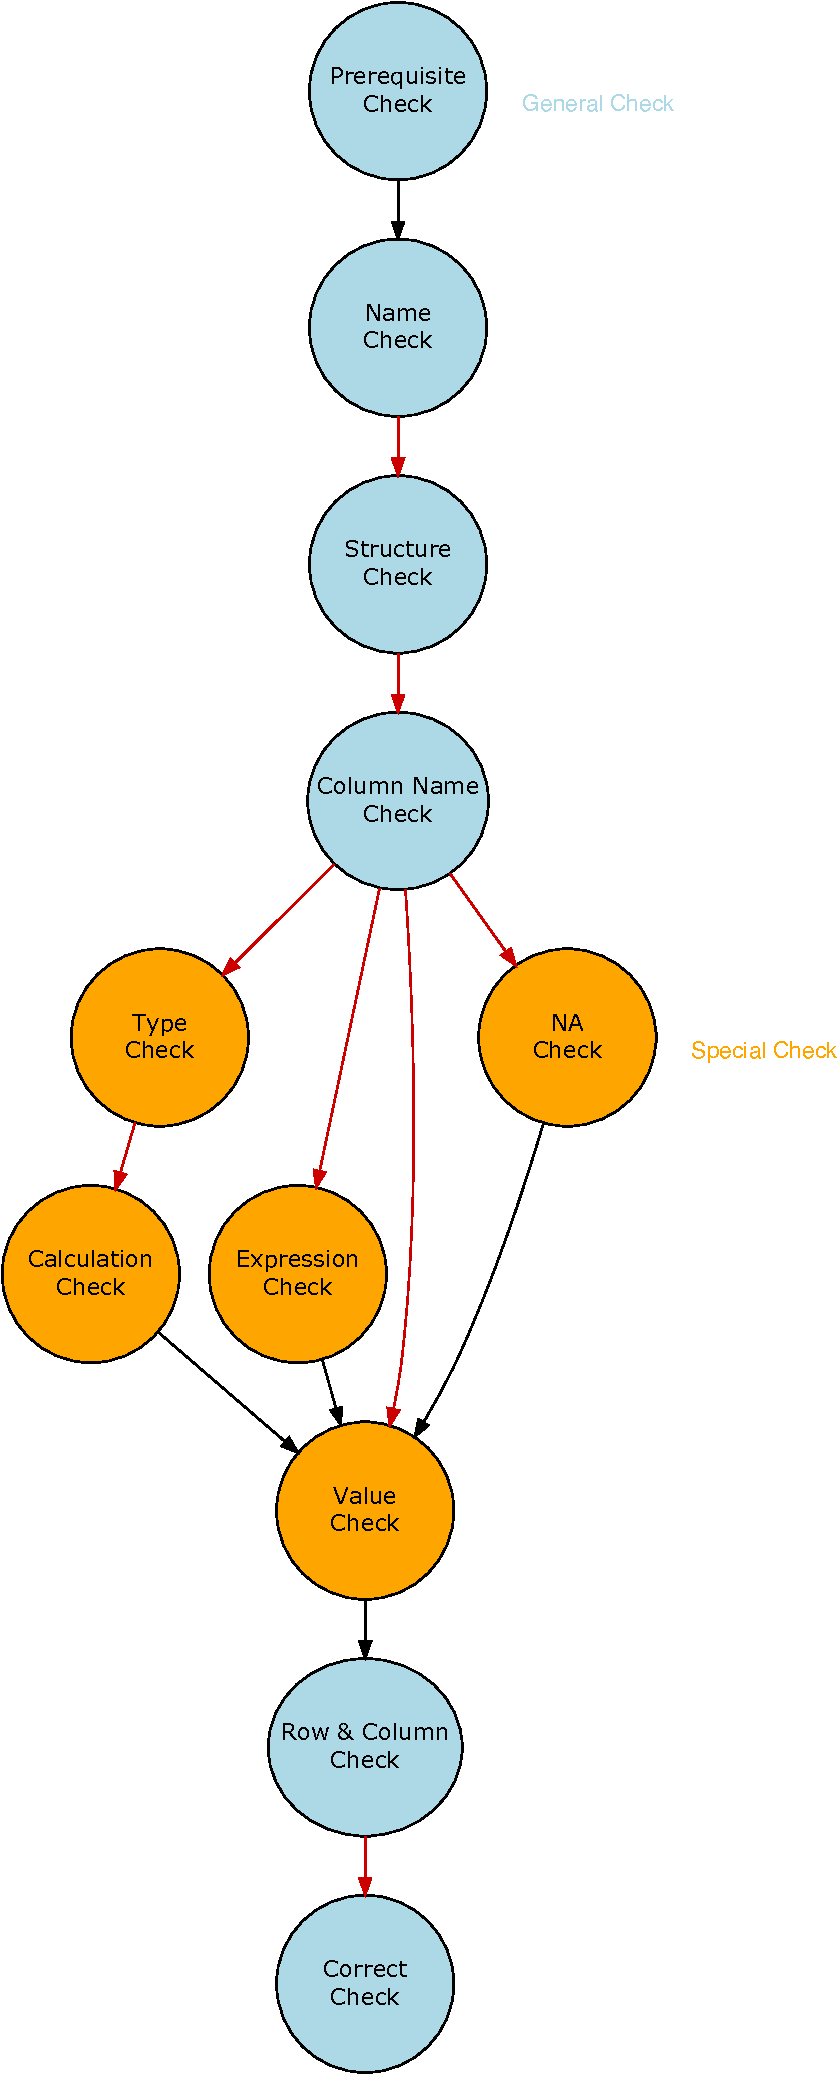
\includegraphics{UCSB-ECON145-AutograderManual_files/figure-latex/unnamed-chunk-28-1} \end{center}

\chapter{Putting It All Together}\label{Putting-It-All-Together}

The following are examples of autograder code for a Public Question involving a tibble, vector, and (named) list respectively, incorporating many of the \hyperref[General-Checks]{General} and \hyperref[Special-Checks]{Special Checks} discussed earlier.

\section{Example: Tibble}\label{example-tibble}

Consider the following question from Homework 9.\footnote{Technically, this is the \emph{fifth} question of the assignment, but I have modified it to be the fourth to align with its question number in \texttt{test.results{[}\#,\ {]}}.}

\textbf{Part 1: Coding Assignment}

\begin{enumerate}
\def\labelenumi{\arabic{enumi}.}
\setcounter{enumi}{3}
\tightlist
\item
  (\emph{Public Question}) Next, using \texttt{un\_data\_tfr} create a new tibble called \textbf{\texttt{un\_data\_tfr\_gdp}} that contains a column for the year, a column for the region, and a column for the average GDP per capita in each region for each year. The new column should be called \textbf{\texttt{gdp\_per\_capita}}, and should be created by dividing the sum of GDP by the sum of population for each region and year.
\end{enumerate}

The answer should look something like:

\begin{Shaded}
\begin{Highlighting}[]
\NormalTok{un\_data\_tfr\_gdp }\OtherTok{\textless{}{-}}\NormalTok{ un\_data\_tfr }\SpecialCharTok{|\textgreater{}}
  \FunctionTok{summarise}\NormalTok{(}\AttributeTok{gdp\_per\_capita =} \FunctionTok{weighted.mean}\NormalTok{(gdp\_per\_capita, population, }\AttributeTok{na.rm =}\NormalTok{ T),}
            \AttributeTok{.by =} \FunctionTok{c}\NormalTok{(year, region))}
\end{Highlighting}
\end{Shaded}

Assume this question is worth 20 points and that \texttt{un\_data\_tfr} was created in Question 2.

Then, the autograder code for this question could look like:

\begin{Shaded}
\begin{Highlighting}[]
\CommentTok{\#Autograder Code for Part 1 Question 4{-}{-}{-}{-}{-}{-}{-}{-}{-}{-}}

\CommentTok{\#Initializing \textasciigrave{}test.results[4, ]\textasciigrave{}}
\NormalTok{test.results[}\DecValTok{4}\NormalTok{, ] }\OtherTok{\textless{}{-}} \FunctionTok{c}\NormalTok{(}\StringTok{"Part 1 Question 4 (Public)"}\NormalTok{, }\DecValTok{0}\NormalTok{, }\DecValTok{20}\NormalTok{, }\StringTok{"Try again. Hint: Start with summarize()."}\NormalTok{)}
  
\CommentTok{\#Prerequisite Check}
\ControlFlowTok{if}\NormalTok{(test.results[}\DecValTok{2}\NormalTok{, }\DecValTok{2}\NormalTok{] }\SpecialCharTok{==} \DecValTok{0}\NormalTok{)\{}
\NormalTok{  test.results[}\DecValTok{4}\NormalTok{, }\DecValTok{4}\NormalTok{] }\OtherTok{\textless{}{-}} \StringTok{"This question depends on \textasciigrave{}un\_data\_tfr\textasciigrave{} from Question 2 being correct. Try again."}
\CommentTok{\#Name Check}
\NormalTok{\} }\ControlFlowTok{else} \ControlFlowTok{if}\NormalTok{(}\FunctionTok{is.error}\NormalTok{(un\_data\_tfr\_gdp))\{}
\NormalTok{  test.results[}\DecValTok{4}\NormalTok{, }\DecValTok{4}\NormalTok{] }\OtherTok{\textless{}{-}} \StringTok{"\textasciigrave{}un\_data\_tfr\_gdp\textasciigrave{} is not found. Please make sure to name the variable correctly. Hint: Check spelling and capitalization."}
\CommentTok{\#Structure Check (for a tibble)}
\NormalTok{\} }\ControlFlowTok{else} \ControlFlowTok{if}\NormalTok{(}\SpecialCharTok{!}\FunctionTok{is\_tibble}\NormalTok{(un\_data\_tfr\_gdp))\{}
\NormalTok{  test.results[}\DecValTok{4}\NormalTok{, }\DecValTok{4}\NormalTok{] }\OtherTok{\textless{}{-}} \StringTok{"\textasciigrave{}un\_data\_tfr\_gdp\textasciigrave{} is not a tibble. Please make sure it is a tibble."}
\CommentTok{\#Column Name Check}
\NormalTok{\} }\ControlFlowTok{else} \ControlFlowTok{if}\NormalTok{(}\SpecialCharTok{!}\FunctionTok{all}\NormalTok{(}\FunctionTok{colnames}\NormalTok{(un\_data\_tfr\_gdp\_test) }\SpecialCharTok{\%in\%} \FunctionTok{colnames}\NormalTok{(un\_data\_tfr\_gdp)))\{}
\NormalTok{  test.results[}\DecValTok{4}\NormalTok{, }\DecValTok{4}\NormalTok{] }\OtherTok{\textless{}{-}} \FunctionTok{paste0}\NormalTok{(}\FunctionTok{c}\NormalTok{(}\StringTok{"The following column(s) should be in un\_data\_tfr\_gdp, but they were not found in your answer:"}\NormalTok{,}
                                 \FunctionTok{colnames}\NormalTok{(un\_data\_tfr\_gdp\_test)[}\SpecialCharTok{!}\NormalTok{(}\FunctionTok{colnames}\NormalTok{(un\_data\_tfr\_gdp\_test) }\SpecialCharTok{\%in\%} \FunctionTok{colnames}\NormalTok{(un\_data\_tfr\_gdp))],}
                                 \StringTok{". Hint: Use summarize() with appropriate .by = argument (besides gdp\_per\_capita, the other two columns that you need will be }
\StringTok{                                 your .by argument, in the form of a vector.)"}\NormalTok{), }\AttributeTok{collapse =} \StringTok{" "}\NormalTok{)}
\NormalTok{\} }\ControlFlowTok{else} \ControlFlowTok{if}\NormalTok{(}\SpecialCharTok{!}\FunctionTok{all}\NormalTok{(}\FunctionTok{colnames}\NormalTok{(un\_data\_tfr\_gdp) }\SpecialCharTok{\%in\%} \FunctionTok{colnames}\NormalTok{(un\_data\_tfr\_gdp\_test)))\{}
\NormalTok{  test.results[}\DecValTok{4}\NormalTok{, }\DecValTok{4}\NormalTok{] }\OtherTok{\textless{}{-}} \FunctionTok{paste0}\NormalTok{(}\FunctionTok{c}\NormalTok{(}\StringTok{"The following column(s) should not be in un\_data\_tfr\_gdp, but they were found in your answer :"}\NormalTok{,}
                                 \FunctionTok{colnames}\NormalTok{(un\_data\_tfr\_gdp)[}\SpecialCharTok{!}\NormalTok{(}\FunctionTok{colnames}\NormalTok{(un\_data\_tfr\_gdp) }\SpecialCharTok{\%in\%} \FunctionTok{colnames}\NormalTok{(un\_data\_tfr\_gdp\_test))],}
                                 \StringTok{". Hint: Use summarize() with appropriate .by= argument (besides gdp\_per\_capita, the other two columns that you need will be }
\StringTok{                                 your .by argument, in the form of a vector.)"}\NormalTok{), }\AttributeTok{collapse =} \StringTok{" "}\NormalTok{)}
\CommentTok{\#NA Check }
\NormalTok{\} }\ControlFlowTok{else} \ControlFlowTok{if}\NormalTok{(}\FunctionTok{sum}\NormalTok{(}\FunctionTok{is.na}\NormalTok{(un\_data\_tfr\_gdp}\SpecialCharTok{$}\NormalTok{gdp\_per\_capita)) }\SpecialCharTok{\textgreater{}} \DecValTok{0}\NormalTok{)\{}
\NormalTok{  test.results[}\DecValTok{4}\NormalTok{, }\DecValTok{4}\NormalTok{] }\OtherTok{\textless{}{-}} \StringTok{"There are \textasciigrave{}NA\textasciigrave{} values in your \textasciigrave{}gdp\_per\_capita\textasciigrave{} column. Hint: You can do one of the following: (1) filter out all rows with missing gdp (or gdp\_per\_capita) and population values first, (2) set na.rm correctly when necessary."}
\CommentTok{\#Type Check (numeric)}
\NormalTok{\} }\ControlFlowTok{else} \ControlFlowTok{if}\NormalTok{(}\SpecialCharTok{!}\FunctionTok{is.numeric}\NormalTok{(un\_data\_tfr\_gdp}\SpecialCharTok{$}\NormalTok{gdp\_per\_capita))\{}
\NormalTok{  test.results[}\DecValTok{4}\NormalTok{, }\DecValTok{4}\NormalTok{] }\OtherTok{\textless{}{-}} \StringTok{"\textasciigrave{}gdp\_per\_capita\textasciigrave{} should be a numeric column."}
\CommentTok{\#Calculation Check }
\NormalTok{\} }\ControlFlowTok{else} \ControlFlowTok{if}\NormalTok{(}\FunctionTok{isTRUE}\NormalTok{(}\FunctionTok{all.equal}\NormalTok{((un\_data\_tfr\_gdp}\SpecialCharTok{$}\NormalTok{gdp\_per\_capita }\SpecialCharTok{/} \DecValTok{1000}\NormalTok{) }\SpecialCharTok{|\textgreater{}} \FunctionTok{sort}\NormalTok{(),}
\NormalTok{                            un\_data\_tfr\_gdp\_test}\SpecialCharTok{$}\NormalTok{gdp\_per\_capita }\SpecialCharTok{|\textgreater{}} \FunctionTok{sort}\NormalTok{())))\{}
\NormalTok{  test.results[}\DecValTok{4}\NormalTok{, }\DecValTok{4}\NormalTok{] }\OtherTok{\textless{}{-}} \StringTok{"The \textasciigrave{}gdp\_per\_capita\textasciigrave{} column is incorrect. Hint: If you used \textasciigrave{}gdp\textasciigrave{} to calculate \textasciigrave{}gdp\_per\_capita\textasciigrave{} column in summarize(), don\textquotesingle{}t forget that \textasciigrave{}population\textasciigrave{} is in terms of thousands of people."}
\CommentTok{\#Value Check }
\NormalTok{\} }\ControlFlowTok{else} \ControlFlowTok{if}\NormalTok{(}\SpecialCharTok{!}\FunctionTok{isTRUE}\NormalTok{(}\FunctionTok{all.equal}\NormalTok{(un\_data\_tfr\_gdp}\SpecialCharTok{$}\NormalTok{gdp\_per\_capita }\SpecialCharTok{|\textgreater{}} \FunctionTok{sort}\NormalTok{(),}
\NormalTok{                            un\_data\_tfr\_gdp\_test}\SpecialCharTok{$}\NormalTok{gdp\_per\_capita }\SpecialCharTok{|\textgreater{}} \FunctionTok{sort}\NormalTok{(),}
                            \AttributeTok{tolerance =} \FloatTok{0.001}\NormalTok{)))\{}
\NormalTok{  test.results[}\DecValTok{4}\NormalTok{, }\DecValTok{4}\NormalTok{] }\OtherTok{\textless{}{-}} \StringTok{"The \textasciigrave{}gdp\_per\_capita\textasciigrave{} column is incorrect. Hint: Within summarize(), try weighted.mean(). Or you can use sum() to implement a weighted average. Note: If you used sum(), you will need to remove rows that have a missing gdp or population value in the first place."}
\CommentTok{\#Row Check }
\NormalTok{\} }\ControlFlowTok{else} \ControlFlowTok{if}\NormalTok{(}\FunctionTok{nrow}\NormalTok{(un\_data\_tfr\_gdp) }\SpecialCharTok{!=} \FunctionTok{nrow}\NormalTok{(un\_data\_tfr\_gdp\_test))\{}
\NormalTok{  test.results[}\DecValTok{4}\NormalTok{, }\DecValTok{4}\NormalTok{] }\OtherTok{\textless{}{-}} \StringTok{"The number of rows in un\_data\_tfr\_gdp is not correct. Hint: Did you use the summarize() function correctly?"}
\CommentTok{\#Correct Check }
\NormalTok{\} }\ControlFlowTok{else} \ControlFlowTok{if}\NormalTok{(}\FunctionTok{isTRUE}\NormalTok{(}\FunctionTok{all.equal}\NormalTok{(un\_data\_tfr\_gdp }\SpecialCharTok{|\textgreater{}} \FunctionTok{ungroup}\NormalTok{() }\SpecialCharTok{|\textgreater{}}
                           \FunctionTok{select}\NormalTok{(}\FunctionTok{colnames}\NormalTok{(un\_data\_tfr\_gdp\_test)) }\SpecialCharTok{|\textgreater{}}
                           \FunctionTok{arrange}\NormalTok{(}\FunctionTok{across}\NormalTok{(}\FunctionTok{everything}\NormalTok{())),}
\NormalTok{                           un\_data\_tfr\_gdp\_test }\SpecialCharTok{|\textgreater{}} \FunctionTok{ungroup}\NormalTok{() }\SpecialCharTok{|\textgreater{}} 
                           \FunctionTok{select}\NormalTok{(}\FunctionTok{colnames}\NormalTok{(un\_data\_tfr\_gdp\_test)) }\SpecialCharTok{|\textgreater{}}
                           \FunctionTok{arrange}\NormalTok{(}\FunctionTok{across}\NormalTok{(}\FunctionTok{everything}\NormalTok{())),}
                           \AttributeTok{tolerance =} \FloatTok{0.001}\NormalTok{,}
                           \AttributeTok{check.attributes =}\NormalTok{ F)))\{}
\NormalTok{  test.results[}\DecValTok{4}\NormalTok{, }\DecValTok{2}\NormalTok{] }\OtherTok{\textless{}{-}} \DecValTok{20}
\NormalTok{  test.results[}\DecValTok{4}\NormalTok{, }\DecValTok{4}\NormalTok{] }\OtherTok{\textless{}{-}} \StringTok{"Well done!"}
\NormalTok{\}}
\end{Highlighting}
\end{Shaded}

\section{Example: Vector}\label{example-vector}

Consider the following question from Homework 2.

\textbf{Part 1: Coding Assignment}

\begin{enumerate}
\def\labelenumi{\arabic{enumi}.}
\setcounter{enumi}{1}
\tightlist
\item
  (\emph{Public Question}) Using the function \texttt{sample}, randomly sample with replacement numbers from \textbf{\texttt{key}} and save this vector as \textbf{\texttt{index}}. The length of \textbf{\texttt{index}} should be 3.
\end{enumerate}

The answer should look something like:

\begin{Shaded}
\begin{Highlighting}[]
\NormalTok{index }\OtherTok{\textless{}{-}} \FunctionTok{sample}\NormalTok{(key, }\AttributeTok{size =} \DecValTok{3}\NormalTok{, }\AttributeTok{replace =} \ConstantTok{TRUE}\NormalTok{)}
\end{Highlighting}
\end{Shaded}

Assume this question is worth 10 points and that \texttt{key} was created in Question 1.

Then, the autograder code for this question could look like:

\begin{Shaded}
\begin{Highlighting}[]
\CommentTok{\#Autograder Code for Part 1 Question 2{-}{-}{-}{-}{-}{-}{-}{-}{-}{-}}
  
\CommentTok{\#Initializing \textasciigrave{}test.results[2, ]\textasciigrave{}}
\NormalTok{test.results[}\DecValTok{2}\NormalTok{, ] }\OtherTok{\textless{}{-}} \FunctionTok{c}\NormalTok{(}\StringTok{"Part 1 Question 2 (Public)"}\NormalTok{, }\DecValTok{0}\NormalTok{, }\DecValTok{10}\NormalTok{, }\StringTok{"Try again."}\NormalTok{)}

\CommentTok{\#Prerequisite Check }
\ControlFlowTok{if}\NormalTok{(test.results[}\DecValTok{1}\NormalTok{, }\DecValTok{2}\NormalTok{] }\SpecialCharTok{==} \DecValTok{0}\NormalTok{)\{}
\NormalTok{  test.results[}\DecValTok{2}\NormalTok{, }\DecValTok{4}\NormalTok{] }\OtherTok{\textless{}{-}} \StringTok{"This problem depends on Part 1 Question 1 being correct. Try again."}
\CommentTok{\#Name Check }
\NormalTok{\} }\ControlFlowTok{else} \ControlFlowTok{if}\NormalTok{(}\FunctionTok{is.error}\NormalTok{(index))\{ }
\NormalTok{  test.results[}\DecValTok{2}\NormalTok{, }\DecValTok{4}\NormalTok{] }\OtherTok{\textless{}{-}} \StringTok{"\textasciigrave{}index\textasciigrave{} is not found. Please make sure your variable is named correctly."}
\CommentTok{\#Structure Check (for a vector)}
\NormalTok{\} }\ControlFlowTok{else} \ControlFlowTok{if}\NormalTok{(}\SpecialCharTok{!}\FunctionTok{is.vector}\NormalTok{(index, }\AttributeTok{mode =} \StringTok{"any"}\NormalTok{))\{ }
\NormalTok{  test.results[}\DecValTok{2}\NormalTok{, }\DecValTok{4}\NormalTok{] }\OtherTok{\textless{}{-}} \StringTok{"Please make sure \textasciigrave{}index\textasciigrave{} is a vector."}
\CommentTok{\#Structure Check (for a numeric vector)}
\NormalTok{\} }\ControlFlowTok{else} \ControlFlowTok{if}\NormalTok{(}\SpecialCharTok{!}\FunctionTok{is.vector}\NormalTok{(index, }\AttributeTok{mode =} \StringTok{"numeric"}\NormalTok{))\{ }
\NormalTok{  test.results[}\DecValTok{2}\NormalTok{, }\DecValTok{4}\NormalTok{] }\OtherTok{\textless{}{-}} \StringTok{"Please make sure \textasciigrave{}index\textasciigrave{} is a numeric vector."}
\CommentTok{\#Length Check (i.e., Row \& Column Check for a vector)}
\NormalTok{\} }\ControlFlowTok{else} \ControlFlowTok{if}\NormalTok{(}\FunctionTok{length}\NormalTok{(index) }\SpecialCharTok{!=} \FunctionTok{length}\NormalTok{(index\_test))\{ }
\NormalTok{  test.results[}\DecValTok{2}\NormalTok{, }\DecValTok{4}\NormalTok{] }\OtherTok{\textless{}{-}} \StringTok{"Please make sure the vector \textasciigrave{}index\textasciigrave{} is the correct length, as specified by the prompt (i.e., there are 3 elements in the vector)."}
\CommentTok{\#Value Check (for a vector)}
\NormalTok{\} }\ControlFlowTok{else} \ControlFlowTok{if}\NormalTok{(}\SpecialCharTok{!}\FunctionTok{all}\NormalTok{(index }\SpecialCharTok{\%in\%}\NormalTok{ index\_test))\{ }
\NormalTok{  test.results[}\DecValTok{2}\NormalTok{, }\DecValTok{4}\NormalTok{] }\OtherTok{\textless{}{-}} \StringTok{"\textasciigrave{}index\textasciigrave{} has incorrect values. Hint: did you use the argument replace = TRUE in the \textasciigrave{}sample()\textasciigrave{} function?"}
\CommentTok{\#Correct Check}
\NormalTok{\} }\ControlFlowTok{else} \ControlFlowTok{if}\NormalTok{(}\FunctionTok{isTRUE}\NormalTok{(}\FunctionTok{all.equal}\NormalTok{(index, index\_test, }
                           \AttributeTok{tolerance =} \FloatTok{0.001}\NormalTok{, }\AttributeTok{check.attributes =}\NormalTok{ F)))\{ }
\NormalTok{  test.results[}\DecValTok{2}\NormalTok{, }\DecValTok{4}\NormalTok{] }\OtherTok{\textless{}{-}} \StringTok{"Well done!"}
\NormalTok{  test.results[}\DecValTok{2}\NormalTok{, }\DecValTok{2}\NormalTok{] }\OtherTok{\textless{}{-}} \DecValTok{10}
\NormalTok{\}}
\end{Highlighting}
\end{Shaded}

\section{Example: List}\label{example-list}

Consider the following question from Homework 7.

\textbf{Part 1: Coding Assignment}

\begin{enumerate}
\def\labelenumi{\arabic{enumi}.}
\setcounter{enumi}{2}
\tightlist
\item
  (\emph{Public Question}) Create a table called \textbf{\texttt{crime\_race\_counts}} that shows the number of crimes along with the percentage of crimes that were committed against victims of each race in \texttt{victim\_race}. Your percentages should be out of 100 and rounded to one decimal place. You should remove any rows that do not record the victim's race.
\end{enumerate}

The answer should look something like:

\begin{Shaded}
\begin{Highlighting}[]
\NormalTok{crime\_race\_counts }\OtherTok{\textless{}{-}}\NormalTok{ crimeData\_clean }\SpecialCharTok{|\textgreater{}} 
  \FunctionTok{filter}\NormalTok{(}\SpecialCharTok{!}\FunctionTok{is.na}\NormalTok{(vict\_race)) }\SpecialCharTok{|\textgreater{}} 
  \FunctionTok{tabyl}\NormalTok{(vict\_race) }\SpecialCharTok{|\textgreater{}}
  \FunctionTok{adorn\_pct\_formatting}\NormalTok{()}
\end{Highlighting}
\end{Shaded}

Assume this question is worth 10 points and that \texttt{crimeData\_clean} was created in Question 1.

Then, the autograder code for this question could look like:

\begin{Shaded}
\begin{Highlighting}[]
\CommentTok{\#Complete Autograder Code for Part 1 Question 3{-}{-}{-}{-}{-}{-}{-}{-}{-}{-}}

\CommentTok{\#Initializing \textasciigrave{}test.results[3, ]\textasciigrave{}}
\NormalTok{test.results[}\DecValTok{3}\NormalTok{, ] }\OtherTok{\textless{}{-}} \FunctionTok{c}\NormalTok{(}\StringTok{"Part 1 Question 3 (Public)"}\NormalTok{, }\DecValTok{0}\NormalTok{, }\DecValTok{10}\NormalTok{, }\StringTok{"Try again. Hint: Look at the function \textasciigrave{}janitor::tabyl()\textasciigrave{}."}\NormalTok{)}
  
\CommentTok{\#Prerequisite Check}
\ControlFlowTok{if}\NormalTok{(test.results[}\DecValTok{1}\NormalTok{, }\DecValTok{2}\NormalTok{] }\SpecialCharTok{==} \DecValTok{0}\NormalTok{)\{}
\NormalTok{  test.results[}\DecValTok{3}\NormalTok{, }\DecValTok{4}\NormalTok{] }\OtherTok{\textless{}{-}} \StringTok{"This question depends on Question 1 being correct. Try again."}
\CommentTok{\#Name Check}
\NormalTok{\} }\ControlFlowTok{else} \ControlFlowTok{if}\NormalTok{(}\FunctionTok{is.error}\NormalTok{(crime\_race\_counts))\{ }
\NormalTok{  test.results[}\DecValTok{3}\NormalTok{, }\DecValTok{4}\NormalTok{] }\OtherTok{\textless{}{-}} \StringTok{"\textasciigrave{}crime\_race\_counts\textasciigrave{} is not found. Please make sure the variable is named correctly."}
\CommentTok{\#Structure Check (for a list)}
\NormalTok{\} }\ControlFlowTok{else} \ControlFlowTok{if}\NormalTok{(}\SpecialCharTok{!}\FunctionTok{is.list}\NormalTok{(crime\_race\_counts))\{}
\NormalTok{  test.results[}\DecValTok{3}\NormalTok{, }\DecValTok{4}\NormalTok{] }\OtherTok{\textless{}{-}} \StringTok{"\textasciigrave{}crime\_race\_counts\textasciigrave{} is not a list. Make sure it is a list. Hint: Look at the function \textasciigrave{}janitor::tabyl()\textasciigrave{}."}
\CommentTok{\#Named List Check (i.e., to make sure the list is named)}
\NormalTok{\} }\ControlFlowTok{else} \ControlFlowTok{if}\NormalTok{(}\FunctionTok{is.null}\NormalTok{(}\FunctionTok{names}\NormalTok{(crime\_race\_counts)))\{}
\NormalTok{    test.results[}\DecValTok{3}\NormalTok{, }\DecValTok{4}\NormalTok{] }\OtherTok{\textless{}{-}} \StringTok{"\textasciigrave{}crime\_race\_counts\textasciigrave{} has no names. Make sure it has names. Hint: Look at the function \textasciigrave{}janitor::tabyl()\textasciigrave{}."}
\CommentTok{\#NA Check}
\NormalTok{\} }\ControlFlowTok{else} \ControlFlowTok{if}\NormalTok{(}\ConstantTok{NA} \SpecialCharTok{\%in\%}\NormalTok{ crime\_race\_counts}\SpecialCharTok{$}\NormalTok{vict\_race)\{}
\NormalTok{    test.results[}\DecValTok{3}\NormalTok{, }\DecValTok{4}\NormalTok{] }\OtherTok{\textless{}{-}} \StringTok{"The column \textasciigrave{}vict\_race\textasciigrave{} contains \textasciigrave{}NA\textasciigrave{} values. Remember to remove any rows which do not record the victim’s race."}
\CommentTok{\#List Name Check (i.e., Column Name Check for a list)}
\NormalTok{\} }\ControlFlowTok{else} \ControlFlowTok{if}\NormalTok{(}\SpecialCharTok{!}\FunctionTok{all}\NormalTok{(}\FunctionTok{names}\NormalTok{(crime\_race\_counts\_test) }\SpecialCharTok{\%in\%} \FunctionTok{names}\NormalTok{(crime\_race\_counts)))\{}
\NormalTok{  test.results[}\DecValTok{3}\NormalTok{, }\DecValTok{4}\NormalTok{] }\OtherTok{\textless{}{-}} \FunctionTok{paste0}\NormalTok{(}\FunctionTok{paste0}\NormalTok{(}\FunctionTok{c}\NormalTok{(}\StringTok{"The following column name(s) should be in \textasciigrave{}crime\_race\_counts\textasciigrave{}, but they were not found in your answer:"}\NormalTok{,}
                               \FunctionTok{names}\NormalTok{(crime\_race\_counts\_test)[}\SpecialCharTok{!}\NormalTok{(}\FunctionTok{names}\NormalTok{(crime\_race\_counts\_test) }\SpecialCharTok{\%in\%} \FunctionTok{names}\NormalTok{(crime\_race\_counts))]),}
                               \AttributeTok{collapse =} \StringTok{"  "}\NormalTok{), }\StringTok{". Hint: Look at the function \textasciigrave{}janitor::tabyl()\textasciigrave{}."}\NormalTok{)}
\NormalTok{\} }\ControlFlowTok{else} \ControlFlowTok{if}\NormalTok{(}\SpecialCharTok{!}\FunctionTok{all}\NormalTok{(}\FunctionTok{names}\NormalTok{(crime\_race\_counts) }\SpecialCharTok{\%in\%} \FunctionTok{names}\NormalTok{(crime\_race\_counts\_test)))\{}
\NormalTok{  test.results[}\DecValTok{3}\NormalTok{, }\DecValTok{4}\NormalTok{] }\OtherTok{\textless{}{-}} \FunctionTok{paste0}\NormalTok{(}\FunctionTok{paste0}\NormalTok{(}\FunctionTok{c}\NormalTok{(}\StringTok{"The following column name(s) should not be in \textasciigrave{}crime\_race\_counts\textasciigrave{}, but they were found in your answer:"}\NormalTok{,}
                                   \FunctionTok{names}\NormalTok{(crime\_race\_counts)[}\SpecialCharTok{!}\NormalTok{(}\FunctionTok{names}\NormalTok{(crime\_race\_counts) }\SpecialCharTok{\%in\%} \FunctionTok{names}\NormalTok{(crime\_race\_counts\_test))]),}
                                 \AttributeTok{collapse =} \StringTok{"  "}\NormalTok{), }\StringTok{". Hint: Look at the function \textasciigrave{}janitor::tabyl()\textasciigrave{}."}\NormalTok{)}
\CommentTok{\#Expression Check (for \% symbol)}
\NormalTok{\} }\ControlFlowTok{else} \ControlFlowTok{if}\NormalTok{(}\FunctionTok{any}\NormalTok{(}\SpecialCharTok{!}\FunctionTok{str\_detect}\NormalTok{(crime\_race\_counts}\SpecialCharTok{$}\NormalTok{percent, }\StringTok{"\%"}\NormalTok{)))\{}
\NormalTok{  test.results[}\DecValTok{3}\NormalTok{, }\DecValTok{4}\NormalTok{] }\OtherTok{\textless{}{-}} \StringTok{"The \textasciigrave{}percent\textasciigrave{} column should be formatted as a percentage. Hint: Look at the function \textasciigrave{}janitor::adorn\_pct\_formatting()\textasciigrave{}."}
\CommentTok{\#Expression Check (for 1 decimal place)}
\NormalTok{\} }\ControlFlowTok{else} \ControlFlowTok{if}\NormalTok{(}\FunctionTok{any}\NormalTok{(}\FunctionTok{str\_detect}\NormalTok{(crime\_race\_counts}\SpecialCharTok{$}\NormalTok{percent, }\StringTok{"}\SpecialCharTok{\textbackslash{}\textbackslash{}}\StringTok{.}\SpecialCharTok{\textbackslash{}\textbackslash{}}\StringTok{d\{2,\}"}\NormalTok{)))\{}
\NormalTok{    test.results[}\DecValTok{3}\NormalTok{, }\DecValTok{4}\NormalTok{] }\OtherTok{\textless{}{-}} \StringTok{"The \textasciigrave{}percent\textasciigrave{} column should be formatted by 1 decimal place. Hint: Look at the argument \textasciigrave{}digits\textasciigrave{} in \textasciigrave{}janitor::adorn\_pct\_formatting()\textasciigrave{} (note its default value)."}
\CommentTok{\#Row \& Column Check (note: the Column Check is redundant here)}
\NormalTok{\} }\ControlFlowTok{else} \ControlFlowTok{if}\NormalTok{(}\FunctionTok{nrow}\NormalTok{(crime\_race\_counts) }\SpecialCharTok{!=} \FunctionTok{nrow}\NormalTok{(crime\_race\_counts\_test))\{}
\NormalTok{  test.results[}\DecValTok{3}\NormalTok{, }\DecValTok{4}\NormalTok{] }\OtherTok{\textless{}{-}} \StringTok{"\textasciigrave{}crime\_race\_counts\textasciigrave{} has the incorrect number of rows. Hint: Look at the \textasciigrave{}janitor::tabyl()\textasciigrave{} function."}
\NormalTok{\} }\ControlFlowTok{else} \ControlFlowTok{if}\NormalTok{(}\FunctionTok{ncol}\NormalTok{(crime\_race\_counts) }\SpecialCharTok{!=} \FunctionTok{ncol}\NormalTok{(crime\_race\_counts\_test))\{ }
\NormalTok{  test.results[}\DecValTok{3}\NormalTok{, }\DecValTok{4}\NormalTok{] }\OtherTok{\textless{}{-}} \StringTok{"\textasciigrave{}crime\_race\_counts\textasciigrave{} has the incorrect number of columns. Hint: Look at the \textasciigrave{}janitor::tabyl()\textasciigrave{} function."}
\CommentTok{\#Correct Check}
\NormalTok{\} }\ControlFlowTok{else} \ControlFlowTok{if}\NormalTok{(}\FunctionTok{isTRUE}\NormalTok{(}\FunctionTok{all.equal}\NormalTok{(crime\_race\_counts }\SpecialCharTok{|\textgreater{}} \FunctionTok{ungroup}\NormalTok{() }\SpecialCharTok{|\textgreater{}} 
                           \FunctionTok{select}\NormalTok{(}\FunctionTok{names}\NormalTok{(crime\_race\_counts\_test)) }\SpecialCharTok{|\textgreater{}}
                           \FunctionTok{arrange}\NormalTok{(}\FunctionTok{across}\NormalTok{(}\FunctionTok{everything}\NormalTok{())),}
\NormalTok{                           crime\_race\_counts\_test }\SpecialCharTok{|\textgreater{}} \FunctionTok{ungroup}\NormalTok{() }\SpecialCharTok{|\textgreater{}}
                           \FunctionTok{select}\NormalTok{(}\FunctionTok{names}\NormalTok{(crime\_race\_counts\_test)) }\SpecialCharTok{|\textgreater{}}
                           \FunctionTok{arrange}\NormalTok{(}\FunctionTok{across}\NormalTok{(}\FunctionTok{everything}\NormalTok{())),}
                           \AttributeTok{tolerance =} \FloatTok{0.001}\NormalTok{,}
                           \AttributeTok{check.attributes =}\NormalTok{ F)))\{}
\NormalTok{    test.results[}\DecValTok{3}\NormalTok{, }\DecValTok{2}\NormalTok{] }\OtherTok{\textless{}{-}} \DecValTok{10}
\NormalTok{    test.results[}\DecValTok{3}\NormalTok{, }\DecValTok{4}\NormalTok{] }\OtherTok{\textless{}{-}} \StringTok{"Well done!"}
\NormalTok{\}  }
\end{Highlighting}
\end{Shaded}

\chapter{Private Questions}\label{Private-Questions}

Private Question Checks are designed to give students \emph{necessary and basic feedback} -- not detailed hints. Their purpose is to flag basic issues without guiding the student toward the solution. Accordingly, Private Question Checks only incorporate \hyperref[General-Checks]{General Checks}.

These Checks help students identify \emph{trivial errors} (e.g., a misspelled column name) and \emph{reduce time debugging}, allowing them to focus on the question's core aspects.

To achieve this, Private Questions are graded using three built-in functions: \texttt{private\_grader()}, \texttt{ggplot\_grader()}, and \texttt{private\_tabyl\_grader()}.\footnote{For ECON 145 TAs, \texttt{private\_grader()}, \texttt{ggplot\_grader()}, and \texttt{private\_tabyl\_grader()} can be found in the subfolder \texttt{helper\_functions/misc\_helper\_functions}.} The following sections explain how to use each function and its parameters.

\begin{infobox}{bell_note}
\textbf{Note}:

Function sample code omit the \hyperref[test.results]{\texttt{test.results{[}\#,\ {]}}} initialization for readability.

Remember to \emph{always} initialize \texttt{test.results{[}\#,\ {]}} before implementing a question's autograder code.

\end{infobox}

\section{private\_grader()}\label{private_grader}

\subsection*{Description}\label{description}
\addcontentsline{toc}{subsection}{Description}

Grades Private Questions involving tibbles, vectors, (named) lists, or plots, providing only basic feedback.

The function implements many of the \hyperref[General-Checks]{General Checks} discussed earlier.

\subsection*{Usage}\label{usage}
\addcontentsline{toc}{subsection}{Usage}

\begin{Shaded}
\begin{Highlighting}[]
\FunctionTok{private\_grader}\NormalTok{(var\_name, }
\NormalTok{               var, }
\NormalTok{               var\_test, }
               \AttributeTok{status =} \FunctionTok{paste0}\NormalTok{(}\StringTok{"Question "}\NormalTok{, quest\_num, }\StringTok{" (Private)"}\NormalTok{), }
               \AttributeTok{var\_status =} \StringTok{"tib"}\NormalTok{, }
               \AttributeTok{prev\_check =} \ConstantTok{TRUE}\NormalTok{, }
               \AttributeTok{is\_tibble\_check =} \ConstantTok{TRUE}\NormalTok{, }
               \AttributeTok{quest\_check\_read =} \ConstantTok{FALSE}\NormalTok{, }
               \AttributeTok{quest\_num =} \DecValTok{0}\NormalTok{, }
               \AttributeTok{quest\_pt =} \DecValTok{0}\NormalTok{,}
               \AttributeTok{quest\_prev =} \DecValTok{1}\NormalTok{, }
               \AttributeTok{quest\_prev\_status =} \ConstantTok{NULL}\NormalTok{)}
\end{Highlighting}
\end{Shaded}

\subsection*{Arguments}\label{arguments}
\addcontentsline{toc}{subsection}{Arguments}

\renewcommand{\arraystretch}{2}

\begin{longtable}{>{\raggedright\arraybackslash}p{4cm}>{\raggedright\arraybackslash}p{8cm}>{\raggedright\arraybackslash}p{4cm}}
\toprule
\textbf{Element} & \textbf{Description} & \textbf{Default}\\
\midrule
\cellcolor{gray!10}{var\_name} & \cellcolor{gray!10}{character, the expected name of var} & \cellcolor{gray!10}{-}\\
\hline
var & expected R object, the student's object & -\\
\hline
\cellcolor{gray!10}{var\_test} & \cellcolor{gray!10}{other R object, the answer key's object to be compared with var} & \cellcolor{gray!10}{-}\\
\hline
status & character, the question's displayed part, number, and type (Private/Public); Example: "Part 2 Question 2 (Private)" & paste0("Question ", quest\_num, " (Private)")\\
\hline
\cellcolor{gray!10}{var\_status} & \cellcolor{gray!10}{the data type of var; Example: "tib" (tibble), "vect" (vector), "lst" (list), "plt" (plot)} & \cellcolor{gray!10}{"tib"}\\
\hline
prev\_check & logical indicating if the Prerequisite Check should be triggered. Requires quest\_prev value and can optionally be combined with quest\_prev\_status & TRUE\\
\hline
\cellcolor{gray!10}{is\_tibble\_check} & \cellcolor{gray!10}{logical indicating if the tibble Structure Check should be triggered} & \cellcolor{gray!10}{TRUE}\\
\hline
quest\_check\_read & logical indicating if the message "Please make sure you are using read\_csv(), not read.csv()." should be attached to the tibble Structure Check & FALSE\\
\hline
\cellcolor{gray!10}{quest\_num} & \cellcolor{gray!10}{numeric, the question's number} & \cellcolor{gray!10}{0}\\
\hline
quest\_pt & numeric, the question's maximum score & 0\\
\hline
\cellcolor{gray!10}{quest\_prev} & \cellcolor{gray!10}{numeric, the prerequisite question's number} & \cellcolor{gray!10}{1}\\
\hline
quest\_prev\_status & character, the prerequisite question's part and number; Example: "Part 2 Question 3b" & NULL\\
\bottomrule
\end{longtable}

\subsection*{Value}\label{value}
\addcontentsline{toc}{subsection}{Value}

The \texttt{test.results{[}\#,\ {]}} vector, containing the question's \texttt{status}, amount of points awarded, total point value, and feedback message.

See \hyperref[test.results]{What is test.results?} for more details.

\subsection*{Details}\label{details}
\addcontentsline{toc}{subsection}{Details}

\begin{infobox}{important_exclamation}
Designed for grading Private Questions involving \textbf{tibbles, vectors, lists, or plots only}.

Plot grading via \texttt{private\_grader()} is limited. Consistent with previous ECON 145 autograders, full credit is awarded if the student simply names the plot properly and gets any prerequisite question correct. For more detailed feedback, consider using the \hyperref[ggplot_grader]{\texttt{ggplot\_grader()}} for ggplot-type questions. See \hyperref[private_grader-plots]{Plots} for more information.

The function grades \textbf{two-way tabyl lists only}. For \hyperref[three-way_tabyl]{three-way tabyl} lists, please use \hyperref[private_tabyl_grader]{\texttt{private\_tabyl\_grader()}} instead.

\end{infobox}

Note that \texttt{var} is the \emph{expected} student's R object and may not necessarily exist (e.g., the student saved their variable under a different name).

\begin{itemize}
\tightlist
\item
  This is not a problem because \texttt{private\_grader()} first performs the \hyperref[Name-Check]{Name Check}. If \texttt{var} does not exist, the subsequent Checks will not be triggered.
\end{itemize}

Also note that \texttt{quest\_prev\_status} is an \emph{optional} argument when setting \texttt{prev\_check} and \texttt{quest\_prev} but helps \emph{clarify} an unclear prerequisite question's location in the feedback message.

\begin{itemize}
\tightlist
\item
  For example, if the prerequisite question is Part 2 Question 3b, but is the eighth question of the assignment (\texttt{quest\_prev\ =\ 8}), this argument can specify its particular location through setting \texttt{quest\_prev\_status\ =\ “Part\ 2\ Question\ 3b”}. Otherwise, its question's number will be displayed (i.e., \texttt{"Question\ 8"}).
\end{itemize}

\subsection*{Example 1: Tibble}\label{example-1-tibble}
\addcontentsline{toc}{subsection}{Example 1: Tibble}

Consider the following questions from Homework 14.

\textbf{Part 1: Coding Assignment}

\begin{enumerate}
\def\labelenumi{\arabic{enumi}.}
\item
  First, you will combine player salary data with CPI data.

  \begin{enumerate}
  \def\labelenumii{(\alph{enumii})}
  \item
    (\emph{Private Question}) Load in the \texttt{Master.csv} file, keeping the columns for player ID, birth year, birth country, first name, last name, weight, height, bats, throws, debut date, and final game date. Save the tibble as \textbf{\texttt{player\_master\_data}}.
  \item
    (\emph{Private Question}) Load in the \texttt{Salaries.csv} file into R. Join the \texttt{player\_master\_data} tibble with the data from \texttt{Salaries.csv} by \texttt{playerID}, keeping only rows with data from both datasets. Save the resulting, joined tibble as \textbf{\texttt{player\_salary\_data1}}.
  \end{enumerate}
\end{enumerate}

Assume each question is worth 5 points.

Then, the autograder code for this question should look like:\footnote{While manipulation of the default parameters can allow \texttt{private\_grader()} to be implemented with fewer explicit inputs, it is recommended to explicitly define \emph{at least} the parameters included in these examples for clarity and consistency.}

\begin{Shaded}
\begin{Highlighting}[]
\CommentTok{\#Comparing the student\textquotesingle{}s tibble \textasciigrave{}player\_master\_data\textasciigrave{} with the answer key\textquotesingle{}s \textasciigrave{}player\_master\_data\_test\textasciigrave{} }
\CommentTok{\#Since this is the first question of the assignment, there is no prerequisite check and so \textasciigrave{}prev\_check\textasciigrave{} is set to \textasciigrave{}FALSE\textasciigrave{}}
\CommentTok{\#Moreover, since this question involves the loading in of a .csv file, it would be helpful to remind students to use \textasciigrave{}read\_csv()\textasciigrave{} and not \textasciigrave{}read.csv()\textasciigrave{} by setting \textasciigrave{}quest\_check\_read\textasciigrave{} to \textasciigrave{}TRUE\textasciigrave{}}
\NormalTok{test.results[}\DecValTok{1}\NormalTok{, ] }\OtherTok{\textless{}{-}} \FunctionTok{private\_grader}\NormalTok{(}\StringTok{"player\_master\_data"}\NormalTok{, player\_master\_data, player\_master\_data\_test,}
                                    \AttributeTok{status =} \StringTok{"Part 1 Question 1a (Private)"}\NormalTok{, }\AttributeTok{var\_status =} \StringTok{"tib"}\NormalTok{,}
                                    \AttributeTok{quest\_check\_read =} \ConstantTok{TRUE}\NormalTok{, }\AttributeTok{prev\_check =} \ConstantTok{FALSE}\NormalTok{, }\AttributeTok{quest\_num =} \DecValTok{1}\NormalTok{, }\AttributeTok{quest\_pt =} \DecValTok{5}\NormalTok{)}

\CommentTok{\#Comparing the student\textquotesingle{}s tibble \textasciigrave{}player\_salary\_data1\textasciigrave{} with the answer key\textquotesingle{}s \textasciigrave{}player\_salary\_data1\_test\textasciigrave{} }
\CommentTok{\#This question relies on the student correctly reproducing \textasciigrave{}player\_master\_data\textasciigrave{} in the previous question, so \textasciigrave{}prev\_check\textasciigrave{}, \textasciigrave{}quest\_prev\textasciigrave{}, and \textasciigrave{}quest\_prev\_status\textasciigrave{} are set appropriately}
\CommentTok{\#Since this question also involves the reading in of data, \textasciigrave{}quest\_check\_read\textasciigrave{} is set to TRUE}
\NormalTok{test.results[}\DecValTok{2}\NormalTok{, ] }\OtherTok{\textless{}{-}} \FunctionTok{private\_grader}\NormalTok{(}\StringTok{"player\_salary\_data1"}\NormalTok{, player\_salary\_data1, player\_salary\_data1\_test,}
                                    \AttributeTok{status =} \StringTok{"Part 1 Question 1b (Private)"}\NormalTok{, }\AttributeTok{var\_status =} \StringTok{"tib"}\NormalTok{,}
                                    \AttributeTok{prev\_check =} \ConstantTok{TRUE}\NormalTok{, }\AttributeTok{quest\_prev =} \DecValTok{1}\NormalTok{, }\AttributeTok{quest\_prev\_status =} \StringTok{"Part 1 Question 1a"}\NormalTok{,}
                                    \AttributeTok{quest\_check\_read =} \ConstantTok{TRUE}\NormalTok{, }\AttributeTok{quest\_num =} \DecValTok{2}\NormalTok{, }\AttributeTok{quest\_pt =} \DecValTok{5}\NormalTok{)}
\end{Highlighting}
\end{Shaded}

\subsection*{Example 2: Vectors}\label{example-2-vectors}
\addcontentsline{toc}{subsection}{Example 2: Vectors}

Consider the following questions from Starter Assignment 1.

\textbf{Part 1: Numeric Object Type and Logical Operators}

\begin{enumerate}
\def\labelenumi{\arabic{enumi}.}
\item
  (\emph{Private Question}) Assign number \texttt{1.45} to the variable \textbf{\texttt{num\_1}}. Remember that the assignment operator in R is \texttt{\textless{}-}.
\item
  (\emph{Private Question}) Assign number \texttt{5} to the variable \textbf{\texttt{num\_2}}.
\end{enumerate}

Assume each question is worth 1 point.

Then, the autograder code for this question should look like:

\begin{Shaded}
\begin{Highlighting}[]
\CommentTok{\#Comparing the student\textquotesingle{}s vector \textasciigrave{}num\_1\textasciigrave{} with the answer key\textquotesingle{}s \textasciigrave{}num\_1\_test\textasciigrave{} }
\CommentTok{\#Since this question does not rely on another question, \textasciigrave{}prev\_check\textasciigrave{} is set to \textasciigrave{}FALSE\textasciigrave{}}
\NormalTok{test.results[}\DecValTok{1}\NormalTok{, ] }\OtherTok{\textless{}{-}} \FunctionTok{private\_grader}\NormalTok{(}\StringTok{"num\_1"}\NormalTok{, num\_1, num\_1\_test,}
                                    \AttributeTok{status =} \StringTok{"Part 1 Question 1 (Private)"}\NormalTok{, }\AttributeTok{var\_status =} \StringTok{"vect"}\NormalTok{,}
                                    \AttributeTok{prev\_check =} \ConstantTok{FALSE}\NormalTok{, }\AttributeTok{quest\_num =} \DecValTok{1}\NormalTok{, }\AttributeTok{quest\_pt =} \DecValTok{1}\NormalTok{)}
  
\CommentTok{\#Comparing the student\textquotesingle{}s vector \textasciigrave{}num\_2\textasciigrave{} with the answer key\textquotesingle{}s \textasciigrave{}num\_2\_test\textasciigrave{} }
\CommentTok{\#\textasciigrave{}prev\_check\textasciigrave{} is set similarly}
\NormalTok{test.results[}\DecValTok{2}\NormalTok{, ] }\OtherTok{\textless{}{-}} \FunctionTok{private\_grader}\NormalTok{(}\StringTok{"num\_2"}\NormalTok{, num\_2, num\_2\_test,}
                                    \AttributeTok{status =} \StringTok{"Part 1 Question 2 (Private)"}\NormalTok{, }\AttributeTok{var\_status =} \StringTok{"vect"}\NormalTok{,}
                                    \AttributeTok{prev\_check =} \ConstantTok{FALSE}\NormalTok{, }\AttributeTok{quest\_num =} \DecValTok{2}\NormalTok{, }\AttributeTok{quest\_pt =} \DecValTok{1}\NormalTok{)}
\end{Highlighting}
\end{Shaded}

\subsection*{Example 3: Lists}\label{example-3-lists}
\addcontentsline{toc}{subsection}{Example 3: Lists}

Consider the following questions from Homework 7.

\textbf{Part 1: Coding Assignment}

\begin{enumerate}
\def\labelenumi{\arabic{enumi}.}
\setcounter{enumi}{7}
\item
  (\emph{Private Question}) Using \texttt{crimeData}, create a table called \textbf{\texttt{age\_bin\_by\_crime\_percentages}} that shows what percent of crime experienced by each age bin that is violent or nonviolent. Your table should have a column each for violent and nonviolent crimes and a row for each age bin as well as a row for the total across all age bins.
\item
  (\emph{Private Question}) Using \texttt{crimeData}, create a table called \textbf{\texttt{crime\_by\_age\_bin\_percentages}} that shows the percent of violent and nonviolent crimes that occurred in each age bin. Your table should have a column for each age bin and a row each for violent and nonviolent crimes. You should also have a row for the total for each age bin.
\end{enumerate}

Assume each question is worth 10 points and that \texttt{crimeData} was created in Question 6.

Then, the autograder code for these questions should look:

\begin{Shaded}
\begin{Highlighting}[]
\CommentTok{\#Note: Tables (especially those created with \textasciigrave{}janitor::tabyl()\textasciigrave{}) should be classified as lists ("lst") when using \textasciigrave{}private\_grader()\textasciigrave{}}

\CommentTok{\#Comparing the student\textquotesingle{}s list \textasciigrave{}age\_bin\_by\_crime\_percentages\textasciigrave{} with the answer key\textquotesingle{}s \textasciigrave{}age\_bin\_by\_crime\_percentages\_test\textasciigrave{} }
\CommentTok{\#Since this question relies on \textasciigrave{}crimeData\textasciigrave{} being correct, \textasciigrave{}prev\_check\textasciigrave{} and \textasciigrave{}quest\_prev\textasciigrave{} are set appropriately (\textasciigrave{}quest\_prev\_status\textasciigrave{} is omitted)}
\NormalTok{test.results[}\DecValTok{8}\NormalTok{, ] }\OtherTok{\textless{}{-}} \FunctionTok{private\_grader}\NormalTok{(}\StringTok{"age\_bin\_by\_crime\_percentages"}\NormalTok{, age\_bin\_by\_crime\_percentages, age\_bin\_by\_crime\_percentages\_test, }
                                    \AttributeTok{status =} \StringTok{"Part 1 Question 8 (Private)"}\NormalTok{, }\AttributeTok{var\_status =} \StringTok{"lst"}\NormalTok{, }
                                    \AttributeTok{prev\_check =} \ConstantTok{TRUE}\NormalTok{, }\AttributeTok{quest\_num =} \DecValTok{8}\NormalTok{, }\AttributeTok{quest\_pt =} \DecValTok{10}\NormalTok{, }\AttributeTok{quest\_prev =} \DecValTok{6}\NormalTok{)}

\CommentTok{\#Comparing the student\textquotesingle{}s list \textasciigrave{}crime\_by\_age\_bin\_percentages\textasciigrave{} with the answer key\textquotesingle{}s \textasciigrave{}crime\_by\_age\_bin\_percentages\_test\textasciigrave{} }
\CommentTok{\#\textasciigrave{}prev\_check\textasciigrave{} and \textasciigrave{}quest\_prev\textasciigrave{} are set appropriately (\textasciigrave{}quest\_prev\_status\textasciigrave{} is omitted)}
\NormalTok{test.results[}\DecValTok{9}\NormalTok{, ] }\OtherTok{\textless{}{-}} \FunctionTok{private\_grader}\NormalTok{(}\StringTok{"crime\_by\_age\_bin\_percentages"}\NormalTok{, crime\_by\_age\_bin\_percentages, crime\_by\_age\_bin\_percentages\_test, }
                                    \AttributeTok{status =} \StringTok{"Part 1 Question 9 (Private)"}\NormalTok{, }\AttributeTok{var\_status =} \StringTok{"lst"}\NormalTok{, }
                                    \AttributeTok{prev\_check =} \ConstantTok{TRUE}\NormalTok{, }\AttributeTok{quest\_num =} \DecValTok{9}\NormalTok{, }\AttributeTok{quest\_pt =} \DecValTok{10}\NormalTok{, }\AttributeTok{quest\_prev =} \DecValTok{6}\NormalTok{)}
\end{Highlighting}
\end{Shaded}

\subsection*{Example 4: Plots}\label{private_grader-plots}
\addcontentsline{toc}{subsection}{Example 4: Plots}

\subsubsection*{Background}\label{background}
\addcontentsline{toc}{subsubsection}{Background}

Previously in ECON 145, plots have not been \emph{rigorously graded} by the autograder due to the desire to award credit to a wide range of students' plots that closely resemble, but are not identical to, the solution.

\begin{itemize}
\item
  Accordingly, \texttt{private\_grader()} only performs the \hyperref[Prerequisite-Check]{Prerequisite Check} and \hyperref[Name-Check]{Name Check} when grading plots. If the student's plot bypasses these Checks, full credit is awarded. Afterwards, plots are \emph{manually graded} by the TAs in the students' write-ups.
\item
  \texttt{ggplot\_grader()} was made in an attempt to provide some level of Checks and feedback for plots created through the \texttt{ggplot2} package. See \hyperref[ggplot_grader]{\texttt{ggplot\_grader()}} for details.
\end{itemize}

Now consider the hypothetical homework question:

\textbf{Part 1: Coding Assignment}

\begin{enumerate}
\def\labelenumi{\arabic{enumi}.}
\setcounter{enumi}{1}
\tightlist
\item
  (\emph{Private Question}) Using \texttt{basketball\_data} from Question 1, create a scatter plot of points (\texttt{pt}) versus assists (\texttt{ast}). Save the plot as \textbf{\texttt{basketball\_scatter}}.
\end{enumerate}

Assume this question is worth 5 points.

Then, the autograder code for this question should look like:

\begin{Shaded}
\begin{Highlighting}[]
\CommentTok{\#Comparing the student\textquotesingle{}s plot \textasciigrave{}basketball\_scatter\textasciigrave{} with the answer key\textquotesingle{}s \textasciigrave{}basketball\_scatter\_test\textasciigrave{} }
\CommentTok{\#Since this question relies on \textasciigrave{}basketball\_data\textasciigrave{} being correct, \textasciigrave{}prev\_check\textasciigrave{} and \textasciigrave{}quest\_prev\textasciigrave{} are set appropriately (\textasciigrave{}quest\_prev\_status\textasciigrave{} is omitted)}
\NormalTok{test.results[}\DecValTok{2}\NormalTok{, ] }\OtherTok{\textless{}{-}} \FunctionTok{private\_grader}\NormalTok{(}\StringTok{"basketball\_scatter"}\NormalTok{, basketball\_scatter, basketball\_scatter\_test,}
                                    \AttributeTok{status =} \StringTok{"Part 1 Question 2 (Private)"}\NormalTok{, }\AttributeTok{var\_status =} \StringTok{"plt"}\NormalTok{,}
                                    \AttributeTok{prev\_check =} \ConstantTok{TRUE}\NormalTok{, }\AttributeTok{quest\_num =} \DecValTok{2}\NormalTok{, }\AttributeTok{quest\_pt =} \DecValTok{5}\NormalTok{, }\AttributeTok{quest\_prev =} \DecValTok{1}\NormalTok{)}
\end{Highlighting}
\end{Shaded}

\subsection*{Acknowledgements}\label{acknowledgements}
\addcontentsline{toc}{subsection}{Acknowledgements}

\textbf{Author}: Riley Berman

\textbf{Contributors}: Alex Zhao, Jack Keefer, Shreya Sinha, Michal Snopek

\section{ggplot\_grader()}\label{ggplot_grader}

\subsection*{Description}\label{description-1}
\addcontentsline{toc}{subsection}{Description}

Grades Private (or Public) Questions involving \texttt{ggplot} objects from the \texttt{ggplot2} package \citep{R-ggplot2}.

This function provides more detailed feedback than traditionally given by the autograder. Rather than evaluating for full plot correctness, \texttt{ggplot\_grader()} checks for key plot attributes, like a proper title or x-y aesthetics, and returns targeted feedback. Accordingly, some flexibility is maintained between the student's plot and the solution.

See \hyperref[private_grader-plots]{Plots} for more information.

\subsection*{Usage}\label{usage-1}
\addcontentsline{toc}{subsection}{Usage}

\begin{Shaded}
\begin{Highlighting}[]
\FunctionTok{ggplot\_grader}\NormalTok{(var\_name, }
\NormalTok{              var, }
\NormalTok{              var\_test, }
              \AttributeTok{status =} \FunctionTok{paste0}\NormalTok{(}\StringTok{"Question "}\NormalTok{, quest\_num, }\StringTok{" (Private)"}\NormalTok{),}
              \AttributeTok{prev\_check =} \ConstantTok{FALSE}\NormalTok{, }
              \AttributeTok{title\_check =} \ConstantTok{FALSE}\NormalTok{, }
              \AttributeTok{axis\_check =} \ConstantTok{FALSE}\NormalTok{, }
              \AttributeTok{aesthetic\_check =} \ConstantTok{FALSE}\NormalTok{, }
              \AttributeTok{aesthetic\_flexible\_check =} \ConstantTok{FALSE}\NormalTok{, }
              \AttributeTok{axis\_name\_check =} \ConstantTok{FALSE}\NormalTok{, }
              \AttributeTok{data\_check =} \ConstantTok{FALSE}\NormalTok{, }
              \AttributeTok{facet\_wrap\_check =} \ConstantTok{FALSE}\NormalTok{, }
              \AttributeTok{geom\_check =} \ConstantTok{FALSE}\NormalTok{, }
              \AttributeTok{geom\_check\_name =} \FunctionTok{c}\NormalTok{(}\StringTok{"GeomPoint"}\NormalTok{), }
              \AttributeTok{color\_fill\_check =} \ConstantTok{FALSE}\NormalTok{, }
              \AttributeTok{color\_fill\_check\_name =} \FunctionTok{c}\NormalTok{(}\StringTok{"colour"}\NormalTok{), }
              \AttributeTok{quest\_num =} \DecValTok{0}\NormalTok{, }
              \AttributeTok{quest\_pt =} \DecValTok{0}\NormalTok{, }
              \AttributeTok{quest\_prev =} \DecValTok{1}\NormalTok{, }
              \AttributeTok{quest\_prev\_status =} \ConstantTok{NULL}\NormalTok{)}
\end{Highlighting}
\end{Shaded}

\subsection*{Arguments}\label{arguments-1}
\addcontentsline{toc}{subsection}{Arguments}

\begin{longtable}{>{\raggedright\arraybackslash}p{4cm}>{\raggedright\arraybackslash}p{8cm}>{\raggedright\arraybackslash}p{4cm}}
\toprule
\textbf{Element} & \textbf{Description} & \textbf{Default}\\
\midrule
\cellcolor{gray!10}{var\_name} & \cellcolor{gray!10}{character, the expected name of var} & \cellcolor{gray!10}{-}\\
\hline
var & expected ggplot object, the student's ggplot & -\\
\hline
\cellcolor{gray!10}{var\_test} & \cellcolor{gray!10}{other ggplot object, the answer key's ggplot to be compared with var} & \cellcolor{gray!10}{-}\\
\hline
status & character, the question’s displayed part, number, and type (Private/Public) & paste0("Question ", quest\_num, " (Private)")\\
\hline
\cellcolor{gray!10}{prev\_check} & \cellcolor{gray!10}{logical indicating if the Prerequisite Check should be triggered; requires quest\_prev value and can optionally be combined with quest\_prev\_status} & \cellcolor{gray!10}{FALSE}\\
\hline
title\_check & logical indicating if an existence check for a graph title should be triggered & FALSE\\
\hline
\cellcolor{gray!10}{axis\_check} & \cellcolor{gray!10}{logical indicating if an existence check for the x-y axis labels should be triggered} & \cellcolor{gray!10}{FALSE}\\
\hline
aesthetic\_check & logical indicating if a strict check for the correct x-y aesthetic mappings should be triggered; alternative to aesthetic\_flexible\_check; see aesthetic\_check or aesthetic\_flexible\_check? & FALSE\\
\hline
\cellcolor{gray!10}{aesthetic\_flexible\_check} & \cellcolor{gray!10}{logical indicating if a flexible check for the correct x-y aesthetic mappings should be triggered; alternative to aesthetic\_check; see aesthetic\_check or aesthetic\_flexible\_check?} & \cellcolor{gray!10}{FALSE}\\
\hline
axis\_name\_check & logical indicating if a check for the correct x-y axis labels should be triggered & FALSE\\
\hline
\cellcolor{gray!10}{data\_check} & \cellcolor{gray!10}{logical indicating if a check for the correct data associated with the x-y aesthetics should be triggered; requires aesthetic\_check} & \cellcolor{gray!10}{FALSE}\\
\hline
facet\_wrap\_check & logical indicating if a check for the existence of ggplot2::facet\_wrap() should be triggered & FALSE\\
\hline
\cellcolor{gray!10}{geom\_check} & \cellcolor{gray!10}{logical indicating if an existence check for ggplot layer types (e.g., ggplot2::geom\_point()) should be triggered; requires geom\_check\_name} & \cellcolor{gray!10}{FALSE}\\
\hline
geom\_check\_name & character vector of the various ggplot layer types to check for in geom\_check; Example: c("GeomPoint", "GeomSmooth") & c("GeomPoint")\\
\hline
\cellcolor{gray!10}{color\_fill\_check} & \cellcolor{gray!10}{logical indicating if an existence check for the "color" and/or "fill" arguments should be triggered; requires color\_fill\_check\_name} & \cellcolor{gray!10}{FALSE}\\
\hline
color\_fill\_check\_name & character vector of the "color" and/or "fill" arguments to check for in color\_fill\_check; Example: c("colour", "fill") & c("colour")\\
\hline
\cellcolor{gray!10}{quest\_num} & \cellcolor{gray!10}{numeric, the question's number} & \cellcolor{gray!10}{0}\\
\hline
quest\_pt & numeric, the question's maximum score & 0\\
\hline
\cellcolor{gray!10}{quest\_prev} & \cellcolor{gray!10}{numeric, the prerequisite question's number} & \cellcolor{gray!10}{1}\\
\hline
quest\_prev\_status & character, the prerequisite question's part and number & NULL\\
\bottomrule
\end{longtable}

\subsection*{Value}\label{value-1}
\addcontentsline{toc}{subsection}{Value}

The \texttt{test.results{[}\#,\ {]}} vector, containing the question's \texttt{status}, amount of points awarded, total point value, and feedback message.

See \hyperref[test.results]{What is test.results?} for more details.

\subsection*{Details}\label{details-1}
\addcontentsline{toc}{subsection}{Details}

\begin{infobox}{important_exclamation}
Designed for grading Private (or Public) Questions involving \textbf{ggplot objects only} (i.e., objects with a \texttt{ggplot} class attribute).

The function flexibly grades ggplot objects by allowing the user to specify which ggplot attributes to check for.

\end{infobox}

Note that \texttt{var} is the \emph{expected} student's ggplot object and may not necessarily exist or be a ggplot object (e.g., the student decided to use R's base \texttt{plot()} instead).

\begin{itemize}
\tightlist
\item
  This is not a problem because \texttt{ggplot\_grader()} first tests for a \texttt{ggplot} class attribute and then performs the \hyperref[Name-Check]{Name Check}. If \texttt{var} does not exist or is not a ggplot object, the subsequent Checks will not be triggered.
\end{itemize}

Like in \hyperref[private_grader]{\texttt{private\_grader()}}, \texttt{quest\_prev\_status} is an \emph{optional} argument when using \texttt{prev\_check} and \texttt{quest\_prev} but helps \emph{clarify} an unclear prerequisite question's location in the feedback message.

Note that for \texttt{color\_fill\_check}, \texttt{colour} is used to set the argument instead of \texttt{color}.

\subsubsection*{When to use aesthetic\_check or aesthetic\_flexible\_check?}\label{aesthetic_check_difference}
\addcontentsline{toc}{subsubsection}{When to use aesthetic\_check or aesthetic\_flexible\_check?}

\texttt{aesthetic\_check} tests if the x-y aesthetic mappings of \texttt{var} are \emph{exactly the same} as in \texttt{var\_test}, while \texttt{aesthetic\_flexible\_check} tests if the x-y aesthetic mappings of \texttt{var\_test} are \emph{contained} in \texttt{var}.

Consider the following motivating example:

\begin{Shaded}
\begin{Highlighting}[]
\CommentTok{\#student\textquotesingle{}s ggplot object}
\NormalTok{var }\OtherTok{\textless{}{-}}\NormalTok{ data }\SpecialCharTok{|\textgreater{}} \FunctionTok{ggplot}\NormalTok{(}\FunctionTok{aes}\NormalTok{(date, death }\SpecialCharTok{*} \DecValTok{100}\NormalTok{)) }

\CommentTok{\#answer key\textquotesingle{}s ggplot object}
\NormalTok{var\_test }\OtherTok{\textless{}{-}}\NormalTok{ data }\SpecialCharTok{|\textgreater{}} \FunctionTok{mutate}\NormalTok{(}\AttributeTok{death =}\NormalTok{ death }\SpecialCharTok{*} \DecValTok{100}\NormalTok{) }\SpecialCharTok{|\textgreater{}} 
            \FunctionTok{ggplot}\NormalTok{(}\FunctionTok{aes}\NormalTok{(date, death)) }
\end{Highlighting}
\end{Shaded}

Under \texttt{aesthetic\_check}, the student's \texttt{var} would \emph{not be considered correct}, because its x-y aesthetic mappings (\texttt{x\ =\ date}, \texttt{y\ =\ death\ *\ 100}) are not the same as in \texttt{var\_test} (\texttt{x\ =\ date}, \texttt{y\ =\ death}), despite the ggplots being \emph{virtually identical.}

However, under \texttt{aesthetic\_flexible\_check}, \texttt{var} is now \emph{considered correct}, since it contains \texttt{var\_test}'s aesthetics.

\begin{infobox}{important_exclamation}
\texttt{aesthetic\_flexible\_check} is more flexible than \texttt{aesthetic\_check}, since it allows for a wider range of acceptable x-y aesthetics. However, because the student's aesthetics can then vary \emph{slightly} from the answer key, the \texttt{data\_check} \textbf{can't be performed without an error occurring.}\footnote{We haven't found any smooth way to fix this, which might entail comparing only the final data used in the ggplot without reference to the x-y aesthetics. The problem we ran into is that to compare the student's and answer key's ggplot data, while allowing for flexible row and column ordering, we need to have \emph{exactly} the same x-y aesthetics. Perhaps something like
  \href{https://ggplot2.tidyverse.org/reference/ggplot_build.html}{\texttt{ggplot\_build}} can resolve this.}

Consequently, \texttt{data\_check} is \emph{automatically} turned off when \texttt{aesthetic\_flexible\_check} is set to \texttt{TRUE}.

\end{infobox}

\textbf{Recommendation}: If it is reasonable that a student could use \emph{similar}, but \emph{not identical}, x-y aesthetics to the solution (like above), use \texttt{aesthetic\_flexible\_check}, keeping in mind that \texttt{data\_check} will be turned off. Otherwise, if the aesthetics can reasonably be expected to be the same as the solution and/or the prompt is explicit about which aesthetics to chose, use \texttt{aesthetic\_check}. Implementing a \texttt{data\_check} is available here.

\begin{itemize}
\tightlist
\item
  Generally, opting for \texttt{aesthetic\_flexible\_check} is the \emph{safer and better choice} (at least until this issue is resolved).
\end{itemize}

\begin{infobox}{warning}
\textbf{Warning}:

\texttt{aesthetic\_flexible\_check} and \texttt{aesthetic\_check} are \emph{mutually exclusive checks.}

\textbf{Do not use both arguments together -- that is, don't set both to \texttt{TRUE}}.

\end{infobox}

\subsection*{Example 1}\label{example-1}
\addcontentsline{toc}{subsection}{Example 1}

Consider the following question from Homework 10.

\textbf{Part 1: COVID-19 Data}

\begin{enumerate}
\def\labelenumi{\arabic{enumi}.}
\setcounter{enumi}{3}
\tightlist
\item
  (\emph{Public Question}) Next, create a bar plot, using \texttt{ggplot2}, that plots the percentage of people who died from COVID-19 based on their vaccination status and age group. The plot should have four bars in two groups. One group of bars should be for those unvaccinated and the second group of bars should be for those vaccinated. In each group, you should have two bars representing the percentage who died of COVID-19, one for those 50 years or older and one for those younger than 50. Save your bar plot as \textbf{\texttt{covid\_plot2}}.
\end{enumerate}

The answer should look something like:

\begin{Shaded}
\begin{Highlighting}[]
\NormalTok{covid\_plot2 }\OtherTok{\textless{}{-}}\NormalTok{ covid\_data }\SpecialCharTok{|\textgreater{}} 
  \FunctionTok{summarize}\NormalTok{(}\AttributeTok{death =} \FunctionTok{sum}\NormalTok{(outcome }\SpecialCharTok{==} \StringTok{"death"}\NormalTok{)}\SpecialCharTok{/}\FunctionTok{n}\NormalTok{(),}
            \AttributeTok{survived =} \FunctionTok{sum}\NormalTok{(outcome }\SpecialCharTok{==} \StringTok{"survived"}\NormalTok{)}\SpecialCharTok{/}\FunctionTok{n}\NormalTok{(),}
            \AttributeTok{.by =} \FunctionTok{c}\NormalTok{(vaccine\_status, age\_group)) }\SpecialCharTok{|\textgreater{}}
    \FunctionTok{ggplot}\NormalTok{(}\FunctionTok{aes}\NormalTok{(}\AttributeTok{x =}\NormalTok{ vaccine\_status, }\AttributeTok{y =}\NormalTok{ death, }\AttributeTok{fill =}\NormalTok{ age\_group)) }\SpecialCharTok{+}
    \FunctionTok{geom\_bar}\NormalTok{(}\AttributeTok{stat =} \StringTok{"identity"}\NormalTok{, }\AttributeTok{position =} \StringTok{"dodge"}\NormalTok{) }\SpecialCharTok{+}
    \FunctionTok{ylab}\NormalTok{(}\StringTok{"percentage"}\NormalTok{) }
\end{Highlighting}
\end{Shaded}

Assume this question is worth 20 points and that we want to check if the ggplot has:

\begin{itemize}
\tightlist
\item
  a \texttt{geom\_bar} layer,
\item
  a \texttt{fill} argument,
\item
  and x-y axis labels.
\end{itemize}

Then, the autograder code for this question should look like:

\begin{Shaded}
\begin{Highlighting}[]
\CommentTok{\#Comparing the student\textquotesingle{}s ggplot \textasciigrave{}covid\_plot2\textasciigrave{} with the answer key\textquotesingle{}s \textasciigrave{}covid\_plot2\_test\textasciigrave{} }
\CommentTok{\#Note: the student can use \textasciigrave{}geom\_col()\textasciigrave{} instead of \textasciigrave{}geom\_bar()\textasciigrave{}, since it has the same ggplot attribute \textasciigrave{}GeomBar\textasciigrave{}}
\NormalTok{test.results[}\DecValTok{4}\NormalTok{, ] }\OtherTok{\textless{}{-}} \FunctionTok{ggplot\_grader}\NormalTok{(}\StringTok{"covid\_plot2"}\NormalTok{, covid\_plot2, covid\_plot2\_test, }
                                   \AttributeTok{status =} \StringTok{"Part 1 Question 4 (Public)"}\NormalTok{, }\AttributeTok{axis\_check =} \ConstantTok{TRUE}\NormalTok{, }
                                   \AttributeTok{geom\_check =} \ConstantTok{TRUE}\NormalTok{, }\AttributeTok{geom\_check\_name =} \FunctionTok{c}\NormalTok{(}\StringTok{"GeomBar"}\NormalTok{), }
                                   \AttributeTok{color\_fill\_check =} \ConstantTok{TRUE}\NormalTok{, }\AttributeTok{color\_fill\_check\_name =} \FunctionTok{c}\NormalTok{(}\StringTok{"fill"}\NormalTok{),}
                                   \AttributeTok{quest\_num =} \DecValTok{4}\NormalTok{, }\AttributeTok{quest\_pt =} \DecValTok{20}\NormalTok{)}
\end{Highlighting}
\end{Shaded}

\subsection*{Example 2}\label{example-2}
\addcontentsline{toc}{subsection}{Example 2}

Consider the following question from Homework 12.

\textbf{Part 1: Coding Assignment}

\begin{enumerate}
\def\labelenumi{\arabic{enumi}.}
\setcounter{enumi}{3}
\item
  In the final coding question, you will recreate Figures 1 and 2, which represent the median home price in the data for each state and the median home price to county per capita income ratio for each state.

  \begin{enumerate}
  \def\labelenumii{\alph{enumii})}
  \setcounter{enumii}{2}
  \tightlist
  \item
    (\emph{Private Question}) Using \texttt{priceIncomeData}, create a bar plot called \textbf{\texttt{priceByIncomePlot}} that shows the median home price to county per capita income ratio for each state and the US as a whole. The x-axis should be the state, and the y-axis should be the median home price to county per capita income ratio. The bars should be colored based on if the state median home price to county per capita income ratio is above or below the US as a whole.
  \end{enumerate}
\end{enumerate}

The answer should look something like:

\begin{Shaded}
\begin{Highlighting}[]
\NormalTok{priceByIncomePlot }\OtherTok{\textless{}{-}}\NormalTok{ priceIncomeData }\SpecialCharTok{|\textgreater{}}
  \FunctionTok{ggplot}\NormalTok{(}\FunctionTok{aes}\NormalTok{(}\AttributeTok{x =} \FunctionTok{reorder}\NormalTok{(state, price\_by\_income), }\AttributeTok{y =}\NormalTok{ price\_by\_income)) }\SpecialCharTok{+}
  \FunctionTok{geom\_bar}\NormalTok{(}\AttributeTok{stat =} \StringTok{"identity"}\NormalTok{, }\FunctionTok{aes}\NormalTok{(}\AttributeTok{fill =}\NormalTok{ above\_below\_us\_price\_by\_income)) }\SpecialCharTok{+}
  \FunctionTok{theme}\NormalTok{(}\AttributeTok{axis.text.x =} \FunctionTok{element\_text}\NormalTok{(}\AttributeTok{angle =} \DecValTok{90}\NormalTok{, }\AttributeTok{hjust =} \DecValTok{1}\NormalTok{)) }\SpecialCharTok{+} \CommentTok{\#rotate x{-}axis values for visibility }
  \FunctionTok{labs}\NormalTok{(}\AttributeTok{title =} \StringTok{\textquotesingle{}Median Home Price to Average Income Ratio\textquotesingle{}}\NormalTok{, }\AttributeTok{x =} \StringTok{\textquotesingle{}State\textquotesingle{}}\NormalTok{, }\AttributeTok{y =} \StringTok{\textquotesingle{}Median Price to Average Income Ratio\textquotesingle{}}\NormalTok{)}
\end{Highlighting}
\end{Shaded}

Assume this question is worth 15 points and is the eighth question of the assignment.

We want to check if the ggplot has:

\begin{itemize}
\tightlist
\item
  a title,
\item
  the correct x-y axis labels,
\item
  a \texttt{geom\_bar} layer,
\item
  a \texttt{fill} argument,
\item
  and a correctly created \texttt{priceIncomeData} from a previous question (the sixth question).
\end{itemize}

Then, the autograder code for this question should look like:

\begin{Shaded}
\begin{Highlighting}[]
\CommentTok{\#Comparing the student\textquotesingle{}s ggplot \textasciigrave{}priceByIncomePlot\textasciigrave{} with the answer key\textquotesingle{}s \textasciigrave{}priceByIncomePlot\_test\textasciigrave{} }
\CommentTok{\#Note: \textasciigrave{}axis\_name\_check\textasciigrave{} can be used without \textasciigrave{}axis\_check\textasciigrave{} to check if the x{-}y axis labels are correct (and therefore exist)}
\NormalTok{test.results[}\DecValTok{8}\NormalTok{, ] }\OtherTok{\textless{}{-}} \FunctionTok{ggplot\_grader}\NormalTok{(}\StringTok{"priceByIncomePlot"}\NormalTok{, priceByIncomePlot, priceByIncomePlot\_test, }
                                   \AttributeTok{status =} \StringTok{"Question 4c (Private)"}\NormalTok{, }\AttributeTok{title\_check =} \ConstantTok{TRUE}\NormalTok{, }
                                   \AttributeTok{axis\_check =} \ConstantTok{TRUE}\NormalTok{, }\AttributeTok{axis\_name\_check =} \ConstantTok{TRUE}\NormalTok{, }
                                   \AttributeTok{geom\_check =} \ConstantTok{TRUE}\NormalTok{, }\AttributeTok{geom\_check\_name =} \FunctionTok{c}\NormalTok{(}\StringTok{"GeomBar"}\NormalTok{), }
                                   \AttributeTok{color\_fill\_check =} \ConstantTok{TRUE}\NormalTok{, }\AttributeTok{color\_fill\_check\_name =} \FunctionTok{c}\NormalTok{(}\StringTok{"fill"}\NormalTok{), }
                                   \AttributeTok{prev\_check =} \ConstantTok{TRUE}\NormalTok{, }\AttributeTok{quest\_prev =} \DecValTok{6}\NormalTok{, }\AttributeTok{quest\_prev\_status =} \StringTok{"Question 4a"}\NormalTok{,}
                                   \AttributeTok{quest\_num =} \DecValTok{8}\NormalTok{, }\AttributeTok{quest\_pt =} \DecValTok{15}\NormalTok{) }
\end{Highlighting}
\end{Shaded}

\subsection*{Example 3}\label{example-3}
\addcontentsline{toc}{subsection}{Example 3}

Consider the following question from Homework 13.

\textbf{Part 1: Coding Assignment}

\begin{enumerate}
\def\labelenumi{\arabic{enumi}.}
\setcounter{enumi}{1}
\item
  In this question, you will work with the \texttt{gdpData.csv} file to analyze national Olympic performance and GDP.

  \begin{enumerate}
  \def\labelenumii{\alph{enumii})}
  \setcounter{enumii}{3}
  \tightlist
  \item
    (\emph{Public Question}) Next, using \texttt{olympic\_gdp\_data} and \texttt{ggplot}, create a group of scatter plots that plot the percentage of the GDP and percentage of the medals won by each country in the 2010 through 2016 Olympic games. The x-axis should contain the percentage of the GDP and the y-axis should contain the percentage of the medals won. The plots should be faceted by the year and season of the Olympic games, such that one plot is for the 2010 winter Olympics, another is for the 2012 summer Olympics, etc. Include a line with slope equal to 1 to denote the values for which the percent of GDP and percent of medals won is equal. You should also label the points on your graph with the NOC codes for the countries that have at least 5\% of the GDP or medals won during each Olympic games. Save your plot as \textbf{\texttt{olympic\_gdp\_perc\_plot}}.
  \end{enumerate}
\end{enumerate}

The answer should look something like:

\begin{Shaded}
\begin{Highlighting}[]
\NormalTok{olympic\_gdp\_perc\_plot }\OtherTok{\textless{}{-}}\NormalTok{ olympic\_gdp\_data }\SpecialCharTok{|\textgreater{}} 
    \FunctionTok{filter}\NormalTok{(year }\SpecialCharTok{\textgreater{}=} \DecValTok{2010}\NormalTok{) }\SpecialCharTok{|\textgreater{}} 
    \FunctionTok{filter}\NormalTok{(}\SpecialCharTok{!}\FunctionTok{is.na}\NormalTok{(gdp\_per\_capita), medalsPerc }\SpecialCharTok{\textgreater{}} \FloatTok{0.001}\NormalTok{) }\SpecialCharTok{|\textgreater{}} 
    \FunctionTok{ggplot}\NormalTok{(}\FunctionTok{aes}\NormalTok{(}\AttributeTok{x =}\NormalTok{ gdpPerc, }\AttributeTok{y =}\NormalTok{ medalsPerc)) }\SpecialCharTok{+} 
    \FunctionTok{geom\_point}\NormalTok{() }\SpecialCharTok{+}
    \FunctionTok{geom\_text}\NormalTok{(}\FunctionTok{aes}\NormalTok{(}\AttributeTok{label =} \FunctionTok{if\_else}\NormalTok{(medalsPerc }\SpecialCharTok{\textgreater{}} \FloatTok{0.05} \SpecialCharTok{|}\NormalTok{ gdpPerc }\SpecialCharTok{\textgreater{}} \FloatTok{0.05}\NormalTok{, noc, }\StringTok{\textquotesingle{}\textquotesingle{}}\NormalTok{), }
                  \AttributeTok{hjust =} \DecValTok{0}\NormalTok{, }\AttributeTok{vjust =} \DecValTok{0}\NormalTok{)) }\SpecialCharTok{+}
    \FunctionTok{geom\_abline}\NormalTok{(}\AttributeTok{intercept =} \DecValTok{0}\NormalTok{, }\AttributeTok{slope =} \DecValTok{1}\NormalTok{, }\AttributeTok{col =} \StringTok{\textquotesingle{}red\textquotesingle{}}\NormalTok{) }\SpecialCharTok{+}
    \FunctionTok{facet\_wrap}\NormalTok{(year}\SpecialCharTok{\textasciitilde{}}\NormalTok{season)}
\end{Highlighting}
\end{Shaded}

Assume that this question is worth 5 points and is the ninth question of the assignment.

We want to check if the ggplot has:

\begin{itemize}
\tightlist
\item
  x-y axis labels,
\item
  the flexibly correct x-y aesthetics,
\item
  \texttt{geom\_point}, \texttt{geom\_abline}, and \texttt{geom\_text} layers,
\item
  a \texttt{facet\_wrap()} function,
\item
  and a correctly created \texttt{olympic\_gdp\_data} from a previous question (the eighth question).
\end{itemize}

Then, the autograder code for this question should look like:

\begin{Shaded}
\begin{Highlighting}[]
\CommentTok{\#Comparing the student\textquotesingle{}s ggplot \textasciigrave{}olympic\_gdp\_perc\_plot\textasciigrave{} with the answer key\textquotesingle{}s \textasciigrave{}olympic\_gdp\_perc\_plot\_test\textasciigrave{} }
\CommentTok{\#Note: \textasciigrave{}geom\_abline()\textasciigrave{} can be checked through the \textasciigrave{}GeomAbline\textasciigrave{} attribute and \textasciigrave{}geom\_text\textasciigrave{} through the \textasciigrave{}GeomText\textasciigrave{} attribute}
\NormalTok{test.results[}\DecValTok{9}\NormalTok{, ] }\OtherTok{\textless{}{-}} \FunctionTok{ggplot\_grader}\NormalTok{(}\StringTok{"olympic\_gdp\_perc\_plot"}\NormalTok{, olympic\_gdp\_perc\_plot , }
\NormalTok{                                   olympic\_gdp\_perc\_plot\_test, }\AttributeTok{status =} \StringTok{"Question 2d (Public)"}\NormalTok{,}
                                   \AttributeTok{axis\_check =} \ConstantTok{TRUE}\NormalTok{, }\AttributeTok{aesthetic\_flexible\_check =} \ConstantTok{TRUE}\NormalTok{, }
                                   \AttributeTok{geom\_check =} \ConstantTok{TRUE}\NormalTok{, }\AttributeTok{geom\_check\_name =} \FunctionTok{c}\NormalTok{(}\StringTok{"GeomPoint"}\NormalTok{, }\StringTok{"GeomAbline"}\NormalTok{, }\StringTok{"GeomText"}\NormalTok{),  }
                                   \AttributeTok{quest\_num =} \DecValTok{9}\NormalTok{, }\AttributeTok{quest\_pt =} \DecValTok{5}\NormalTok{, }\AttributeTok{facet\_wrap\_check =} \ConstantTok{TRUE}\NormalTok{,}
                                   \AttributeTok{prev\_check =} \ConstantTok{TRUE}\NormalTok{, }\AttributeTok{quest\_prev =} \DecValTok{8}\NormalTok{, }\AttributeTok{quest\_prev\_status =} \StringTok{"Question 2c (Public)"}\NormalTok{)}
\end{Highlighting}
\end{Shaded}

\subsection*{Example 4}\label{example-4}
\addcontentsline{toc}{subsection}{Example 4}

Consider the hypothetical homework question:

\textbf{Part 1: Coding Assignment}

\begin{enumerate}
\def\labelenumi{\arabic{enumi}.}
\setcounter{enumi}{1}
\tightlist
\item
  (\emph{Private Question}) Using \texttt{basketball\_data} from Question 1, create a scatter plot of points versus assists with \texttt{ggplot}. The x-axis should be \texttt{pt} and the y-axis should be \texttt{ast.} Save the ggplot as \textbf{\texttt{basketball\_scatter}}.
\end{enumerate}

The answer should look something like:

\begin{Shaded}
\begin{Highlighting}[]
\NormalTok{basketball\_scatter }\OtherTok{\textless{}{-}}\NormalTok{ basketball\_data }\SpecialCharTok{|\textgreater{}} 
  \FunctionTok{ggplot}\NormalTok{(}\FunctionTok{aes}\NormalTok{(}\AttributeTok{x =}\NormalTok{ pt, }\AttributeTok{y =}\NormalTok{ ast)) }\SpecialCharTok{+}
  \FunctionTok{geom\_point}\NormalTok{()}
\end{Highlighting}
\end{Shaded}

Assume this question is worth 5 points and that we want to check if the ggplot has:

\begin{itemize}
\tightlist
\item
  the correct x-y axis labels,
\item
  the correct x-y aesthetics,
\item
  the correct x-y data,
\item
  a \texttt{geom\_point} layer,
\item
  and a correctly created \texttt{basketball\_data} from a previous question (the first question).
\end{itemize}

Then, the autograder code for this question should look like:

\begin{Shaded}
\begin{Highlighting}[]
\CommentTok{\#Comparing the student\textquotesingle{}s plot \textasciigrave{}basketball\_scatter\textasciigrave{} with the answer key\textquotesingle{}s \textasciigrave{}basketball\_scatter\_test\textasciigrave{} }
\NormalTok{test.results[}\DecValTok{2}\NormalTok{, ] }\OtherTok{\textless{}{-}} \FunctionTok{ggplot\_grader}\NormalTok{(}\StringTok{"basketball\_scatter"}\NormalTok{, basketball\_scatter, basketball\_scatter\_test,}
                                    \AttributeTok{status =} \StringTok{"Part 1 Question 2 (Private)"}\NormalTok{, }\AttributeTok{axis\_name\_check =} \ConstantTok{TRUE}\NormalTok{, }
                                    \AttributeTok{aesthetic\_check =} \ConstantTok{TRUE}\NormalTok{, }\AttributeTok{data\_check =} \ConstantTok{TRUE}\NormalTok{,}
                                    \AttributeTok{geom\_check =} \ConstantTok{TRUE}\NormalTok{, }\AttributeTok{geom\_check\_name =} \FunctionTok{c}\NormalTok{(}\StringTok{"GeomPoint"}\NormalTok{), }
                                    \AttributeTok{quest\_num =} \DecValTok{2}\NormalTok{, }\AttributeTok{quest\_pt =} \DecValTok{5}\NormalTok{, }\AttributeTok{prev\_check =} \ConstantTok{TRUE}\NormalTok{, }\AttributeTok{quest\_prev =} \DecValTok{1}\NormalTok{)}
\end{Highlighting}
\end{Shaded}

\subsection*{Acknowledgements}\label{acknowledgements-1}
\addcontentsline{toc}{subsection}{Acknowledgements}

\textbf{Author}: Riley Berman

\textbf{Contributors}: Alex Zhao, Jack Keefer, Shreya Sinha, Michal Snopek

\section{private\_tabyl\_grader()}\label{private_tabyl_grader}

\subsection*{Description}\label{description-2}
\addcontentsline{toc}{subsection}{Description}

Grades Private Questions involving \hyperref[three-way_tabyl]{three-way \texttt{tabyl}} objects from the \texttt{janitor} package \citep{R-janitor}.

This function implements many of the \hyperref[General-Checks]{General Checks} discussed earlier.

\subsection*{Usage}\label{usage-2}
\addcontentsline{toc}{subsection}{Usage}

\begin{Shaded}
\begin{Highlighting}[]
\FunctionTok{private\_tabyl\_grader}\NormalTok{(var\_name, }
\NormalTok{                     var, }
\NormalTok{                     var\_test, }
                     \AttributeTok{status =} \FunctionTok{paste0}\NormalTok{(}\StringTok{"Question "}\NormalTok{, quest\_num, }\StringTok{" (Private)"}\NormalTok{), }
                     \AttributeTok{prev\_check =} \ConstantTok{TRUE}\NormalTok{, }
                     \AttributeTok{quest\_num =} \DecValTok{0}\NormalTok{, }
                     \AttributeTok{quest\_pt =} \DecValTok{0}\NormalTok{, }
                     \AttributeTok{quest\_prev =} \DecValTok{1}\NormalTok{, }
                     \AttributeTok{quest\_prev\_status =} \ConstantTok{NULL}\NormalTok{)}
\end{Highlighting}
\end{Shaded}

\subsection*{Arguments}\label{arguments-2}
\addcontentsline{toc}{subsection}{Arguments}

\begin{longtable}{>{\raggedright\arraybackslash}p{4cm}>{\raggedright\arraybackslash}p{8cm}>{\raggedright\arraybackslash}p{4cm}}
\toprule
\textbf{Element} & \textbf{Description} & \textbf{Default}\\
\midrule
\cellcolor{gray!10}{var\_name} & \cellcolor{gray!10}{character, the expected name of var} & \cellcolor{gray!10}{-}\\
\hline
var & expected tabyl object, the student's tabyl & -\\
\hline
\cellcolor{gray!10}{var\_test} & \cellcolor{gray!10}{other tabyl object, the answer key's tabyl to be compared with var} & \cellcolor{gray!10}{-}\\
\hline
status & character, the question's displayed part, number, and type (Private/Public) & paste0("Question ", quest\_num, " (Private)")\\
\hline
\cellcolor{gray!10}{prev\_check} & \cellcolor{gray!10}{logical indicating if the Prerequisite Check should be triggered; requires quest\_prev value and can optionally be combined with quest\_prev\_status} & \cellcolor{gray!10}{TRUE}\\
\hline
quest\_num & numeric, the question's number & 0\\
\hline
\cellcolor{gray!10}{quest\_pt} & \cellcolor{gray!10}{numeric, the question's maximum score} & \cellcolor{gray!10}{0}\\
\hline
quest\_prev & numeric, the prerequisite question's number & 1\\
\hline
\cellcolor{gray!10}{quest\_prev\_status} & \cellcolor{gray!10}{character, the prerequisite question's part and number} & \cellcolor{gray!10}{NULL}\\
\bottomrule
\end{longtable}

\subsection*{Value}\label{value-2}
\addcontentsline{toc}{subsection}{Value}

The \texttt{test.results{[}\#,\ {]}} vector, containing the question's \texttt{status}, amount of points awarded, total point value, and feedback message.

See \hyperref[test.results]{What is test.results?} for more details.

\subsection*{Details}\label{details-2}
\addcontentsline{toc}{subsection}{Details}

Designed for grading \textbf{three-way tabyl objects only} (i.e., objects with a \texttt{tabyl} class attribute).

Use \hyperref[private_grader]{\texttt{private\_grader()}} for two-way tabyl objects.

As with the other functions, \texttt{var} may not necessarily exist or be a tabyl object.

\begin{itemize}
\tightlist
\item
  This is not a problem because \texttt{private\_tabyl\_grader()} first tests for a \texttt{tabyl} class attribute and then performs the \hyperref[Name-Check]{Name Check}.
\end{itemize}

Likewise, \texttt{quest\_prev\_status} is an optional argument when using \texttt{prev\_check} and \texttt{quest\_prev} but helps \emph{clarify} an unclear prerequisite question's location in the feedback message.

\subsubsection*{What is a three-way tabyl?}\label{three-way_tabyl}
\addcontentsline{toc}{subsubsection}{What is a three-way tabyl?}

A three-way tabyl is a multi-table created from three variables that is produced by the \texttt{janitor::tabyl()} function.

A three-way tabyl will typically create two ``sub-tables.''

Consider the following example from the \texttt{tabyl} documentation \citep{janitortabyls}:

\begin{Shaded}
\begin{Highlighting}[]
\NormalTok{t3 }\OtherTok{\textless{}{-}}\NormalTok{ starwars }\SpecialCharTok{|\textgreater{}}
  \FunctionTok{filter}\NormalTok{(species }\SpecialCharTok{==} \StringTok{"Human"}\NormalTok{) }\SpecialCharTok{|\textgreater{}}
  \FunctionTok{tabyl}\NormalTok{(eye\_color, skin\_color, gender)}

\CommentTok{\#The result is a tabyl of eye color x skin color, split into a list by gender}
\end{Highlighting}
\end{Shaded}

\begin{verbatim}
## $feminine
##  eye_color dark fair light none pale tan white
##       blue    0    2     1    0    0   0     0
##  blue-gray    0    0     0    0    0   0     0
##      brown    0    1     3    0    0   0     0
##       dark    0    0     0    0    0   0     0
##      hazel    0    0     1    0    0   0     0
##    unknown    0    0     0    1    0   0     0
##     yellow    0    0     0    0    0   0     0
## 
## $masculine
##  eye_color dark fair light none pale tan white
##       blue    0    7     2    0    0   0     0
##  blue-gray    0    1     0    0    0   0     0
##      brown    3    4     3    0    0   2     0
##       dark    1    0     0    0    0   0     0
##      hazel    0    1     0    0    0   0     0
##    unknown    0    0     0    0    0   0     0
##     yellow    0    0     0    0    1   0     1
\end{verbatim}

\subsection*{Example}\label{example}
\addcontentsline{toc}{subsection}{Example}

Consider the following modified question from the Final.

\textbf{Part 3: Creating Tables and Figures}

\begin{enumerate}
\def\labelenumi{\arabic{enumi})}
\tightlist
\item
  (\emph{Private Question}) Using \texttt{schoolData}, create a table that shows the percentage of schools that provide free lunch to all students, and how for each year in each \texttt{locale} category (City, Suburb, Town, and Rural). Make sure you remove any rows with missing \texttt{national\_school\_lunch\_program} or \texttt{locale} values before creating your table. Save this table as \textbf{\texttt{nslp\_locale\_table}}.
\end{enumerate}

The answer should look something like:

\begin{Shaded}
\begin{Highlighting}[]
\CommentTok{\#Note: This has been slightly modified from the actual solution}
\NormalTok{nslp\_locale\_table }\OtherTok{\textless{}{-}}\NormalTok{ schoolData }\SpecialCharTok{|\textgreater{}} 
  \FunctionTok{filter}\NormalTok{(}\SpecialCharTok{!}\FunctionTok{is.na}\NormalTok{(locale) }\SpecialCharTok{\&} \SpecialCharTok{!}\FunctionTok{is.na}\NormalTok{(national\_school\_lunch\_program)) }\SpecialCharTok{|\textgreater{}} 
\NormalTok{  janitor}\SpecialCharTok{::}\FunctionTok{tabyl}\NormalTok{(year, national\_school\_lunch\_program, locale) }\SpecialCharTok{|\textgreater{}} 
\NormalTok{  janitor}\SpecialCharTok{::}\FunctionTok{adorn\_percentages}\NormalTok{() }\SpecialCharTok{|\textgreater{}} 
\NormalTok{  janitor}\SpecialCharTok{::}\FunctionTok{adorn\_pct\_formatting}\NormalTok{()}
\end{Highlighting}
\end{Shaded}

Assume this question is worth 5 points, is the sixteenth question of the assignment, and that \texttt{schoolData} was created in Part 1 Question 1b (the second question).

Then, the autograder code for this question should look like:

\begin{Shaded}
\begin{Highlighting}[]
\CommentTok{\#Comparing the student\textquotesingle{}s three{-}way tabyl \textasciigrave{}nslp\_locale\_table\textasciigrave{} with the answer key\textquotesingle{}s \textasciigrave{}nslp\_locale\_table\_test\textasciigrave{} }
\NormalTok{test.results[}\DecValTok{16}\NormalTok{, ] }\OtherTok{\textless{}{-}} \FunctionTok{private\_tabyl\_grader}\NormalTok{(}\StringTok{"nslp\_locale\_table"}\NormalTok{, nslp\_locale\_table, nslp\_locale\_table\_test, }
                                           \AttributeTok{status =} \StringTok{"Part 3 Question 1 (Private)"}\NormalTok{, }\AttributeTok{prev\_check =} \ConstantTok{TRUE}\NormalTok{, }
                                           \AttributeTok{quest\_prev =} \DecValTok{2}\NormalTok{, }\AttributeTok{quest\_prev\_status =} \StringTok{"Part 1 Question 1b"}\NormalTok{, }
                                           \AttributeTok{quest\_num =} \DecValTok{16}\NormalTok{, }\AttributeTok{quest\_pt =} \DecValTok{5}\NormalTok{)}
\end{Highlighting}
\end{Shaded}

\subsection*{Acknowledgements}\label{acknowledgements-2}
\addcontentsline{toc}{subsection}{Acknowledgements}

\textbf{Co-authors}: Michal Snopek, Riley Berman

\textbf{Contributors}: Alex Zhao, Jack Keefer, Shreya Sinha

\chapter{DGP.R}\label{DGP.R}

In the autograder system, the \texttt{DGP.R} file assigns each student a unique dataset drawn from the \texttt{masterdata} according to their PERMID.

See \texttt{00-manual1.pdf} and the \hyperref[PERMID-Check]{PERMID Check} for more information.

\begin{infobox}{bell_note}
\textbf{Note}:

The Head TA determines the sampling method for each assignment. TAs are \emph{only} responsible for implementing this sampling technique in \texttt{DGP.R}.

In some cases, the file does not require any edits.

\end{infobox}

\section{Examples}\label{examples}

A few examples of \texttt{DGP.R} are provided below.

\subsection*{Example 1}\label{example-1-1}
\addcontentsline{toc}{subsection}{Example 1}

\textbf{Description}: Randomly assign each student 1,000 observations sampled from \texttt{masterdata}.

\begin{Shaded}
\begin{Highlighting}[]
\NormalTok{DGP }\OtherTok{\textless{}{-}} \ControlFlowTok{function}\NormalTok{(}\AttributeTok{masterdata =} \StringTok{"Masterdata.csv"}\NormalTok{, }\AttributeTok{PERMID =}\NormalTok{ PERMID, }\AttributeTok{dataname =}\NormalTok{ dataname)\{}
\NormalTok{  masterdata }\OtherTok{\textless{}{-}} \FunctionTok{read\_csv}\NormalTok{(masterdata)}
  \FunctionTok{set.seed}\NormalTok{(PERMID)}
  \CommentTok{\#{-}{-}{-}{-}{-}{-}{-}{-}{-}{-}{-}{-}{-}{-}{-}\#}
  \CommentTok{\#Edit made here... }
\NormalTok{  d }\OtherTok{\textless{}{-}}\NormalTok{ masterdata[}\FunctionTok{sample}\NormalTok{(}\DecValTok{1}\SpecialCharTok{:}\FunctionTok{nrow}\NormalTok{(masterdata), }\DecValTok{1000}\NormalTok{, }\AttributeTok{replace =}\NormalTok{ F),]}
  \CommentTok{\#{-}{-}{-}{-}{-}{-}{-}{-}{-}{-}{-}{-}{-}{-}{-}\#}
\NormalTok{  readr}\SpecialCharTok{::}\FunctionTok{write\_csv}\NormalTok{(d, dataname)}
\NormalTok{\}}
\end{Highlighting}
\end{Shaded}

\subsection*{Example 2}\label{example-2-1}
\addcontentsline{toc}{subsection}{Example 2}

\textbf{Description}: Assign the full \texttt{masterdata} to each student (no sampling). This results in all students receiving the same dataset (adapted from Homework 4).

\begin{Shaded}
\begin{Highlighting}[]
\NormalTok{DGP }\OtherTok{\textless{}{-}} \ControlFlowTok{function}\NormalTok{(}\AttributeTok{masterdata =} \StringTok{"Masterdata.csv"}\NormalTok{, }\AttributeTok{PERMID =}\NormalTok{ PERMID, }\AttributeTok{dataname =}\NormalTok{ dataname)\{}
\NormalTok{  masterdata }\OtherTok{\textless{}{-}} \FunctionTok{read\_csv}\NormalTok{(masterdata)}
  \FunctionTok{set.seed}\NormalTok{(PERMID)}
  \CommentTok{\#{-}{-}{-}{-}{-}{-}{-}{-}{-}{-}{-}{-}{-}{-}{-}\#}
  \CommentTok{\#Edit made here... }
\NormalTok{  d }\OtherTok{\textless{}{-}}\NormalTok{ masterdata}
  \CommentTok{\#{-}{-}{-}{-}{-}{-}{-}{-}{-}{-}{-}{-}{-}{-}{-}\#}
\NormalTok{  readr}\SpecialCharTok{::}\FunctionTok{write\_csv}\NormalTok{(d, dataname)}
\NormalTok{\}}
\end{Highlighting}
\end{Shaded}

\subsection*{Example 3}\label{example-3-1}
\addcontentsline{toc}{subsection}{Example 3}

\textbf{Description}: Randomly assign each student 20,000 observations sampled from every \texttt{masterdata} \emph{except} for the \texttt{masterdata} corresponding to \texttt{datasetB.csv}.\footnote{Sometimes, multiple csv files are required for an assignment, creating multiple \texttt{masterdata}. The \texttt{DGP.R} file will then loop through each \texttt{masterdata}.}

For the \texttt{masterdata} corresponding to \texttt{datasetB.csv}, assign each student the full \texttt{masterdata}. Assume that \texttt{datasetB.csv} has exactly two columns, \texttt{col\_1} and \texttt{col\_2} (adapted from Homework 7).

\begin{Shaded}
\begin{Highlighting}[]
\NormalTok{DGP }\OtherTok{\textless{}{-}} \ControlFlowTok{function}\NormalTok{(}\AttributeTok{masterdata =} \StringTok{"Masterdata.csv"}\NormalTok{, }\AttributeTok{PERMID =}\NormalTok{ PERMID, }\AttributeTok{dataname =}\NormalTok{ dataname)\{}
\NormalTok{  masterdata }\OtherTok{\textless{}{-}} \FunctionTok{read\_csv}\NormalTok{(masterdata)}
  \FunctionTok{set.seed}\NormalTok{(PERMID)}
  \CommentTok{\#{-}{-}{-}{-}{-}{-}{-}{-}{-}{-}{-}{-}{-}{-}{-}\#}
  \CommentTok{\#Edit made here... }
  \CommentTok{\#No sampling for datasetB.csv... }
  \ControlFlowTok{if}\NormalTok{(}\FunctionTok{all}\NormalTok{(}\FunctionTok{colnames}\NormalTok{(masterdata) }\SpecialCharTok{\%in\%} \FunctionTok{c}\NormalTok{(}\StringTok{"col\_1"}\NormalTok{, }\StringTok{"col\_2"}\NormalTok{)))\{}
\NormalTok{    d }\OtherTok{\textless{}{-}}\NormalTok{ masterdata}
  \CommentTok{\#Everything else is randomly sampled...}
\NormalTok{  \} }\ControlFlowTok{else}\NormalTok{\{}
\NormalTok{    d }\OtherTok{\textless{}{-}}\NormalTok{ masterdata[}\FunctionTok{sample}\NormalTok{(}\DecValTok{1}\SpecialCharTok{:}\FunctionTok{nrow}\NormalTok{(masterdata), }\DecValTok{20000}\NormalTok{, }\AttributeTok{replace =}\NormalTok{ F),]}
\NormalTok{  \}}
  \CommentTok{\#{-}{-}{-}{-}{-}{-}{-}{-}{-}{-}{-}{-}{-}{-}{-}\#}
\NormalTok{  readr}\SpecialCharTok{::}\FunctionTok{write\_csv}\NormalTok{(d, dataname)}
\NormalTok{\}}
\end{Highlighting}
\end{Shaded}

\subsection*{Example 4}\label{example-4-1}
\addcontentsline{toc}{subsection}{Example 4}

\textbf{Description}: For the following \texttt{masterdata}, assign as follows:

\begin{itemize}
\item
  \texttt{data1.csv}: Randomly sample 10,000 rows.
\item
  \texttt{data2.csv}: Randomly sample 20,000 rows.
\item
  \texttt{data3.csv}: Assign the full dataset, arrange by its column \texttt{data3\_col2} (so every student will get their dataset in this format).
\item
  \texttt{data4.csv}: Assign the full dataset.
\end{itemize}

Assume \texttt{data1.csv} has some unique column \texttt{data1\_unique\_column} and that \texttt{data2\_col1}, \ldots{} ,\texttt{data2\_col5} are the \emph{only} columns in \texttt{data2.csv} and \texttt{data3\_col1} and \texttt{data3\_col2} are the \emph{only} columns in \texttt{data3.csv} (adapted from Homework 14).

\begin{Shaded}
\begin{Highlighting}[]
\NormalTok{DGP }\OtherTok{\textless{}{-}} \ControlFlowTok{function}\NormalTok{(}\AttributeTok{masterdata =} \StringTok{"Masterdata.csv"}\NormalTok{, }\AttributeTok{PERMID =}\NormalTok{ PERMID, }\AttributeTok{dataname =}\NormalTok{ dataname)\{}
\NormalTok{  masterdata }\OtherTok{\textless{}{-}} \FunctionTok{read\_csv}\NormalTok{(masterdata)}
  \FunctionTok{set.seed}\NormalTok{(PERMID)}
  \CommentTok{\#{-}{-}{-}{-}{-}{-}{-}{-}{-}{-}{-}{-}{-}{-}{-}\#}
  \CommentTok{\#Edit made here... }
  \CommentTok{\#\textasciigrave{}data1.csv\textasciigrave{} randomly sampled for 10,000 observations }
  \ControlFlowTok{if}\NormalTok{(}\StringTok{"data1\_unique\_column"} \SpecialCharTok{\%in\%} \FunctionTok{colnames}\NormalTok{(masterdata))\{}
\NormalTok{    d }\OtherTok{\textless{}{-}}\NormalTok{ masterdata[}\FunctionTok{sample}\NormalTok{(}\DecValTok{1}\SpecialCharTok{:}\FunctionTok{nrow}\NormalTok{(masterdata), }\DecValTok{10000}\NormalTok{, }\AttributeTok{replace =}\NormalTok{ F),]}
  \CommentTok{\#\textasciigrave{}data2.csv\textasciigrave{} randomly sampled for 20,000 observations }
\NormalTok{  \} }\ControlFlowTok{else} \ControlFlowTok{if}\NormalTok{(}\FunctionTok{all}\NormalTok{(}\FunctionTok{colnames}\NormalTok{(masterdata) }\SpecialCharTok{\%in\%} \FunctionTok{c}\NormalTok{(}\StringTok{"data2\_col1"}\NormalTok{, }\StringTok{"data2\_col2"}\NormalTok{, }
                                            \StringTok{"data2\_col3"}\NormalTok{, }\StringTok{"data2\_col4"}\NormalTok{, }\StringTok{"data2\_col5"}\NormalTok{)))\{ }
\NormalTok{    d }\OtherTok{\textless{}{-}}\NormalTok{ masterdata[}\FunctionTok{sample}\NormalTok{(}\DecValTok{1}\SpecialCharTok{:}\FunctionTok{nrow}\NormalTok{(masterdata), }\DecValTok{20000}\NormalTok{, }\AttributeTok{replace =}\NormalTok{ F),]}
  \CommentTok{\#\textasciigrave{}data3.csv\textasciigrave{} is not sampled and is arranged by \textasciigrave{}data3\_col2\textasciigrave{}}
\NormalTok{  \} }\ControlFlowTok{else} \ControlFlowTok{if}\NormalTok{(}\FunctionTok{all}\NormalTok{(}\FunctionTok{colnames}\NormalTok{(masterdata) }\SpecialCharTok{\%in\%} \FunctionTok{c}\NormalTok{(}\StringTok{"data3\_col1"}\NormalTok{, }\StringTok{"data3\_col2"}\NormalTok{)))\{}
\NormalTok{    d }\OtherTok{\textless{}{-}}\NormalTok{ masterdata }\SpecialCharTok{\%\textgreater{}\%} \FunctionTok{arrange}\NormalTok{(data3\_col2)}
  \CommentTok{\#\textasciigrave{}data4.csv\textasciigrave{} is not sampled}
\NormalTok{  \} }\ControlFlowTok{else}\NormalTok{\{}
\NormalTok{    d }\OtherTok{\textless{}{-}}\NormalTok{ masterdata[}\FunctionTok{sample}\NormalTok{(}\DecValTok{1}\SpecialCharTok{:}\FunctionTok{nrow}\NormalTok{(masterdata), }\FunctionTok{nrow}\NormalTok{(masterdata), }\AttributeTok{replace =}\NormalTok{ F),]}
\NormalTok{  \}}
  \CommentTok{\#{-}{-}{-}{-}{-}{-}{-}{-}{-}{-}{-}{-}{-}{-}{-}\#}
\NormalTok{  readr}\SpecialCharTok{::}\FunctionTok{write\_csv}\NormalTok{(d, dataname)}
\NormalTok{\}}
\end{Highlighting}
\end{Shaded}

\subsection*{Example 5}\label{example-5}
\addcontentsline{toc}{subsection}{Example 5}

\textbf{Description}: Assign each student a dataset containing observations from 140 randomly selected countries from \texttt{masterdata}'s \texttt{Country\ or\ Area} column (adapted from Homework 8).

\begin{Shaded}
\begin{Highlighting}[]
\NormalTok{DGP }\OtherTok{\textless{}{-}} \ControlFlowTok{function}\NormalTok{(}\AttributeTok{masterdata =} \StringTok{"Masterdata.csv"}\NormalTok{, }\AttributeTok{PERMID =}\NormalTok{ PERMID, }\AttributeTok{dataname =}\NormalTok{ dataname)\{}
\NormalTok{  masterdata }\OtherTok{\textless{}{-}} \FunctionTok{read\_csv}\NormalTok{(masterdata)}
  \FunctionTok{set.seed}\NormalTok{(PERMID)}
  \CommentTok{\#{-}{-}{-}{-}{-}{-}{-}{-}{-}{-}{-}{-}{-}{-}{-}\#}
  \CommentTok{\#Edit made here... }
  \CommentTok{\#Creating a list of all the countries in \textasciigrave{}masterdata\textasciigrave{}}
\NormalTok{  country\_list }\OtherTok{\textless{}{-}} \FunctionTok{unique}\NormalTok{(masterdata}\SpecialCharTok{$}\StringTok{\textasciigrave{}}\AttributeTok{Country or Area}\StringTok{\textasciigrave{}}\NormalTok{)}
  \CommentTok{\#Randomly selecting 140 countries}
\NormalTok{  country\_sample }\OtherTok{\textless{}{-}} \FunctionTok{sample}\NormalTok{(country\_list, }\DecValTok{140}\NormalTok{)}
  \CommentTok{\#Selecting the rows from \textasciigrave{}masterdata\textasciigrave{} that contain the selected countries}
\NormalTok{  d }\OtherTok{\textless{}{-}}\NormalTok{ masterdata[masterdata}\SpecialCharTok{$}\StringTok{\textasciigrave{}}\AttributeTok{Country or Area}\StringTok{\textasciigrave{}} \SpecialCharTok{\%in\%}\NormalTok{ country\_sample, ]}
  \CommentTok{\#{-}{-}{-}{-}{-}{-}{-}{-}{-}{-}{-}{-}{-}{-}{-}\#}
\NormalTok{  readr}\SpecialCharTok{::}\FunctionTok{write\_csv}\NormalTok{(d, dataname)}
\NormalTok{\}}
\end{Highlighting}
\end{Shaded}

\chapter{Resources}\label{resources}

This is a list of additional resources for ECON 145 TAs to familiarize themselves with the autograder system and implementation.

These links will direct you to the ECON 145 \emph{private} repository on GitHub. You will need to have been invited to the repository to access them.

\begin{itemize}
\item
  \href{https://github.com/datawranglingUCSBecon/econ_145/blob/master/manuals/autograder_quickstart_ta/autograder_presentation.mp4}{autograder\_presentation.mp4}: A recorded presentation given by Alex Zhao and Riley Berman on the technical aspects of setting up, testing, and finalizing autograders through GitHub.
\item
  \href{https://github.com/datawranglingUCSBecon/econ_145/blob/master/manuals/autograder_quickstart_ta/how_to_create_an_autograder_2024.pdf}{how\_to\_create\_an\_autograder\_2024.pdf}: A pdf version of the presentation slides.
\item
  \href{https://github.com/datawranglingUCSBecon/econ_145/blob/master/manuals/autograder_ta/00-manual1.pdf}{00-manual1.pdf}: A comprehensive manual about the entire autograder system. Especially useful for Head TAs.
\end{itemize}

  \bibliography{book.bib,packages.bib}

\end{document}
